\documentclass[twocolumn]{bmcart}% uncomment this for twocolumn layout and comment line below
%\documentclass{bmcart}

%%% Load packages
\usepackage{etex}
\usepackage{epsfig}
\usepackage{amsmath}
\usepackage{multirow}
\usepackage{tabularx}
\usepackage{booktabs}
\usepackage{amsmath,graphicx}
\usepackage{pgf}
\usepackage{tikz}
\usepackage[caption=no]{subfig}
\usetikzlibrary{backgrounds,shapes,snakes}
\usetikzlibrary{calc,chains,positioning}
\usepackage{phaistos}
\usepackage{cases}
\usepackage{pgfplots}
%\usepackage{empheq}
\usepackage{cite}
\usepackage{url}

\begin{document}

\newlength\figureheight
\newlength\figurewidth
\setlength\figureheight{3cm}
\setlength\figurewidth{0.37\textwidth}

%%% Start of article front matter
\begin{frontmatter}

\begin{fmbox}
\dochead{Research}

\title{Improving the Conditioning of the Optimization Criterion in Acoustic Multi-Channel Equalization}


\author[
   addressref={aff1},                   % id's of addresses, e.g. {aff1,aff2}
   corref={aff1},                       % id of corresponding address, if any
   email={ina.kodrasi@uni-oldenburg.de}   % email address
]{\inits{IK}\fnm{Ina} \snm{Kodrasi}}
\author[
   addressref={aff1},
   email={simon.doclo@uni-oldenburg.de}
]{\inits{SD}\fnm{Simon} \snm{Doclo}}

\address[id=aff1]{%                           % unique id
  \orgname{Department of Medical Physics and Acoustics and Cluster of Excellence Hearing4All}, % university, etc
  \street{University of Oldenburg},                     %
  %\postcode{}                                % post or zip code
  \city{Oldenburg},                              % city
  \cny{Germany}                                    % country
}

%\end{fmbox}% comment this for two column layout

%%%%%%%%%%%%%%%%%%%%%%%%%%%%%%%%%%%%%%%%%%%%%%
%%                                          %%
%% The Abstract begins here                 %%
%%                                          %%
%% Please refer to the Instructions for     %%
%% authors on http://www.biomedcentral.com  %%
%% and include the section headings         %%
%% accordingly for your article type.       %%
%%                                          %%
%%%%%%%%%%%%%%%%%%%%%%%%%%%%%%%%%%%%%%%%%%%%%%

\begin{abstractbox}

  \begin{abstract} % abstract
    In least-squares acoustic multi-channel equalization techniques, i.e., the multiple-input/output inverse theorem~(MINT), relaxed multi-channel least-squares~(RMCLS), and partial multi-channel equalization based on MINT~(PMINT), the length of the reshaping filters is generally chosen such that perfect dereverberation is achieved for perfectly estimated room impulse responses~(RIRs).
    Since in practice however the available RIRs typically differ from the true ones, this choice of the reshaping filter length may not be optimal.
    This paper proposes to increase the robustness of equalization techniques against RIR perturbations by using a shorter reshaping filter length than conventionally used, such that a better conditioned optimization criterion is obtained.
    Based on the condition number of the convolution matrix of the RIRs, a mathematical link between the reshaping filter length and the robustness against RIR perturbations is established.
 It is shown that shorter reshaping filters than conventionally used yield a smaller condition number, i.e., a higher robustness against RIR perturbations.
    In addition, we propose a novel automatic non-intrusive procedure for determining the reshaping filter length based on the L-curve.
    Simulation results using measured RIRs confirm that using a shorter reshaping filter length than conventionally used yields a significant increase in robustness against RIR perturbations for the MINT, RMCLS, and PMINT techniques.
    Furthermore, it is shown that the PMINT technique using an optimal intrusively determined reshaping filter length outperforms all other considered techniques in terms of perceptual speech quality.
    Finally, it is shown that the automatic non-intrusively determined reshaping filter length in the PMINT technique yields a similar performance as the optimal intrusively determined reshaping filter length. 
\end{abstract}

%%%%%%%%%%%%%%%%%%%%%%%%%%%%%%%%%%%%%%%%%%%%%%
%%                                          %%
%% The keywords begin here                  %%
%%                                          %%
%% Put each keyword in separate \kwd{}.     %%
%%                                          %%
%%%%%%%%%%%%%%%%%%%%%%%%%%%%%%%%%%%%%%%%%%%%%%

\begin{keyword}
\kwd{speech dereverberation}
\kwd{condition number}
\kwd{reshaping filter length}
\kwd{L-curve}
\end{keyword}


\end{abstractbox}
%
\end{fmbox}% uncomment this for twcolumn layout

\end{frontmatter}

\section{Introduction}
The microphone signals recorded in many hands-free communication applications, such as teleconferencing, voice-controlled systems, or hearing aids, do not only contain the desired speech signal but also attenuated and delayed copies due to reverberation.
Reverberation degrades the intelligibility of the speech signal~\cite{Beutelmann_2006,Warzybok_IWAENC_2014} as well as the performance of automatic speech recognition systems~\cite{Yoshioka_ISPM_2012,Xiong_EURASIP_2015}.

In order to mitigate these detrimental effects of reverberation, several single- and multi-channel dereverberation techniques have been proposed~\cite{Naylor_Derev_book}, with multi-channel techniques being generally preferred since they exploit both the spectro-temporal and the spatial characteristics of the received microphone signals.
Existing multi-channel dereverberation techniques can be broadly classified into spectral enhancement techniques~\cite{Lebart_ACUSTICA_2001,Habets2009a,Braun_EURASIP_2015,Kuklasinski_ITASLP_2016}, probabilistic modelling-based techniques~\cite{Nakatani_ITASLP_2010,Schmid_ITASLP_2014,Schwartz_ITASLP_2015,Jukic_ITASLP_2015}, and acoustic multi-channel equalization techniques~\cite{Miyoshi_ITASS_1988, Kallinger_ICASSP_2006,Jungmann_ITASLP_2012, Hikichi_EURASIP_2007, Lim_ITASLP_2014, Kodrasi_ITASLP_2013, Rashobh_ITASLP_2014}.
Acoustic multi-channel equalization techniques aim to reshape the available room impulse responses (RIRs) between the speaker and the microphone array.
They can in theory achieve perfect dereverberation~\cite{Miyoshi_ITASS_1988,Hacihabibouglu_ITASLP_2012}, and hence, comprise an attractive approach to speech dereverberation.

A well-known multi-channel equalization technique aiming at acoustic system inversion is the multiple-input/output inverse theorem~(MINT) technique~\cite{Miyoshi_ITASS_1988}, which however suffers from drawbacks in practice. 
Since the available RIRs typically differ from the true RIRs due to fluctuations~(e.g., temperature or position variations~\cite{Radlovic_ITSA_2000}) or due to the sensitivity of blind system identification~(BSI) and supervised system identification~(SSI) methods to near-common zeros or interfering noise~\cite{Khong_ICASSP_2008,Haque_SPL_2008,Hu_EUSIPCO_2015}, MINT fails to invert the true RIRs, possibly leading to severe distortions in the output signal~\cite{Hikichi_EURASIP_2007,Kodrasi_ITASLP_2013,Lim_ITASLP_2014}.
In order to increase the robustness against RIR perturbations, partial multi-channel equalization techniques such as relaxed multi-channel least-squares~(RMCLS)~\cite{Lim_ITASLP_2014} and partial multi-channel equalization based on MINT~(PMINT)~\cite{Kodrasi_ITASLP_2013} have been recently proposed. 
Since early reflections tend to improve speech intelligibility~\cite{Arweiler_JASA_2011,Warzybok_JASA_2012} and late reflections are the major cause of speech intelligibility degradation, the objective of these techniques is to shorten the overall impulse response by suppressing only the late reflections.
While RMCLS imposes no constraints on the remaining early reflections, PMINT is more perceptually advantageous since it aims to also control the remaining early reflections.
Although partial equalization techniques can be significantly more robust than MINT, their performance still remains rather susceptible to RIR perturbations~\cite{Lim_ITASLP_2014,Kodrasi_ITASLP_2013}.

The length of the reshaping filters in MINT, RMCLS, and PMINT has been conventionally chosen such that perfect dereverberation can be achieved for perfectly estimated RIRs.
Since in practice the available RIRs typically differ from the true ones, this choice of the reshaping filter length yields a high sensitivity of acoustic multi-channel equalization techniques to RIR perturbations.
In this paper we propose to increase the robustness by decreasing the reshaping filter length, such that a better conditioned optimization criterion is obtained.
A mathematical link between the reshaping filter length and the condition number of the multi-channel convolution matrix of the available RIRs, hence, the sensitivity of equalization techniques to RIR perturbations, is derived. 
We show that shorter reshaping filters than conventionally used yield a smaller condition number, i.e., a higher robustness against RIR perturbations.
Although this result is rather intuitive, to the best of our knowledge it has not been mathematically analysed or investigated in the context of acoustic multi-channel equalization.
In general, the optimal reshaping filter length yielding the highest performance needs to be determined intrusively (i.e., using a dereverberated reference signal and knowledge of the true RIRs), limiting the practical applicability of using shorter reshaping filter lengths in acoustic multi-channel equalization techniques.
In this paper, we also propose and investigate an automatic non-intrusive selection procedure for the reshaping filter length based on the L-curve~\cite{Castellanos_2002}.
Some preliminary results on using shorter reshaping filters in acoustic multi-channel equalization techniques are presented in~\cite{Kodrasi_EUSIPCO_2012}.

Simulation results for several measured acoustic systems and RIR perturbations show by means of instrumental measures that using shorter reshaping filters in MINT, RMCLS, and PMINT significantly increases the robustness against RIR perturbations.
In addition, it is demonstrated that the P-MINT technique using the optimal intrusively determined reshaping filter length outperforms the other considered techniques, yielding a high reverberant energy suppression and perceptual speech quality improvement.
Furthermore, it is shown that the non-intrusively determined reshaping filter length yields a nearly optimal performance in P-MINT, making this technique a practically applicable multi-channel equalization technique for speech dereverberation.

The paper is organized as follows.
In Section~\ref{sec: conf} the considered acoustic configuration and the used notation is introduced.
In Section~\ref{sec: ame} state-of-the-art least-squares acoustic multi-channel equalization techniques, i.e., MINT, RMCLS, and PMINT, are briefly reviewed.
In Section~\ref{sec: cond_no} their sensitivity to RIR perturbations is evaluated by means of the condition number and analytical insights on increasing the robustness by decreasing the reshaping filter length are provided.
In Section~\ref{sec: lauto} the automatic procedure for determining the reshaping filter length is discussed.
Using instrumental measures, the dereverberation performance of all considered techniques is compared in Section~\ref{sec: exp}.

\section{Configuration and notation}
\label{sec: conf}
We consider an acoustic system with a single speech source and $M$ microphones, as depicted in Figure~\ref{fig: ac_sys}.
The $m$-th microphone signal, $m = 1, \; 2, \; \ldots, \; M,$ at time index $n$ is given by
\begin{align}
  y_m(n) &= \underbrace{h_m(n) \ast s(n)}_{x_m(n)} + v_m(n)  \\
  & = x_m(n) + v_m(n),
\end{align}
where $\ast$ denotes convolution, $s(n)$ is the clean speech signal, $h_m(n)$ is the RIR between the source and the $m$-th microphone, $x_{m}(n)$ is the reverberant speech component, and $v_{m}(n)$ is the noise component.
Since acoustic multi-channel equalization techniques generally design dereverberation filters disregarding the presence of the additive noise, in the following it is assumed that $v_m(n) = 0$, hence, $y_m(n) = x_m(n)$.
\begin{figure}[t]
  \centering
  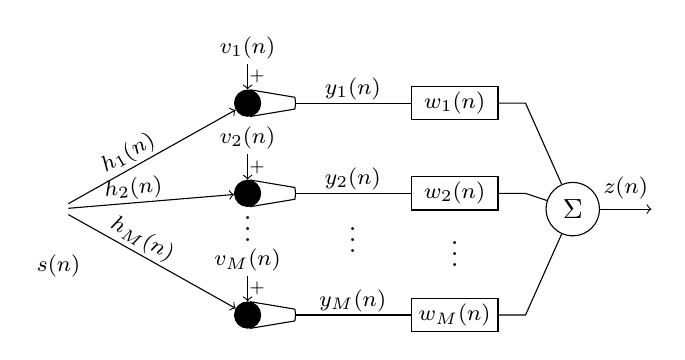
\begin{tikzpicture}
    % Adjustments
    \def\micd{.1cm}                % mic diameter
    \def\micl{.6cm}                % mic length
    \def\micw{.15cm}                % mic width
    \def\micbend{10}               % mic bottom bend
    \def\micdistance{.8cm}         % distance between microphones
    \def\filterdistance{1.9cm}     % distance between microphone and filter
    \def\filteroutline{.9cm}       % length of line which gets out of filter
    \def\sumdistance{1.5cm}        % distance of sum node to the filter
    \def\sumoutline{1cm}           % length of line which gets out of sum
    \def\headdistance{2.4cm}       % distance between microphone and head
    % Styles
    \tikzset{%
      mic head/.style={fill=black,draw=black,circle,minimum size=\micd},
      filter/.style={draw,minimum width=1.1cm,inner sep=2pt},
      sum/.style={draw,circle},
      xlabel/.style={inner sep=1pt,above,midway},
      sumlabel/.style={xlabel},
      hlabel/.style={xlabel,sloped,pos=.4},
      head/.style={font=\Large}
    }%
    % Draw Microphones
    \begin{scope}[start chain=going below,every node/.style={on chain},node distance=\micdistance]
      \node[mic head] (mic1) {};
      \node[mic head] (mic2) {};
      \node[mic head,yshift=-0.5*\micdistance] (mic3) {};
    \end{scope}
    \node[yshift=12pt] at ($(mic2)!.5!(mic3)$) {$\vdots$};
    \foreach \m in {1,2,3} {%
      \coordinate (m1) at ($(mic\m)+(\micl,\micw/2)$);
      \coordinate (m2) at ($(mic\m)+(\micl,-\micw/2)$);
      \draw (tangent cs:node=mic\m,point={(m1)},solution=1) -- (m1) to[bend left=\micbend] (m2) -- (tangent cs:node=mic\m,point={(m2)},solution=2);
    }%
    % Draw Filter
    \foreach \m/\i in {1/1,2/2,3/M} {%
      \node[filter,right=\filterdistance of mic\m] (filter\m) {\footnotesize $w_{\i}(n)$};
      \draw ($(mic\m)+(\micl,0)$) to node[xlabel] (x\m) {\footnotesize $y_{\i}(n)$} (filter\m);
    }%
    \node[yshift=3pt] at ($(filter2)!.5!(filter3)$) {$\vdots$};
    \node[yshift=3pt] at ($(x2)!.5!(x3)$) {$\vdots$};
    % Sum Node %
    \node[sum] (sum) at ($(filter1)!.5!(filter3)+(\sumdistance,0)$) {$\Sigma$};
    \draw[->] (sum) -- node[above] {\footnotesize $z(n)$} ++(1.0,0);
    % Connect filter with sum %
    \foreach \m in {1,2,3} {%
      \draw (filter\m) -- ++(\filteroutline,0) -- (sum);
    }%
    % Head
    \node[head] (head) at ($(mic1)!.5!(mic3)-(\headdistance,0)$) {\PHtattooedHead};
    \node[fill=white,minimum width=4.8pt,minimum height=5.7pt,inner sep=0pt] at ($(head.center)+(2.3pt,-2.5pt)$) {};
    \node at ($(head.center)+(0.0pt,-20.5pt)$) {\footnotesize $s(n)$};
    % Connect head with mics
    \foreach \m/\i in {1/1,2/2,3/M} {%
      \draw[->] (head) -- node[hlabel] {\footnotesize $h_{\i}(n)$} (mic\m);
    }%
    % Draw noise
    \draw[<-] (mic1) -- node[above=0.1cm] {\footnotesize $v_1(n)$} node[right = -0.1cm] {\footnotesize ${}_{+}$} ++(0,0.5);
    \draw[<-] (mic2) -- node[above=0.1cm] {\footnotesize $v_2(n)$} node[right = -0.1cm] {\footnotesize ${}_{+}$} ++(0,0.5);
    \draw[<-] (mic3) -- node[above=0.1cm] {\footnotesize $v_M(n)$} node[right = -0.1cm] {\footnotesize ${}_{+}$} ++(0,0.5);
  \end{tikzpicture}
  \caption{Acoustic system configuration.}
  \label{fig: ac_sys}
\end{figure}

Using the filter-and-sum structure in Figure~\ref{fig: ac_sys}, the output signal $z(n)$ is equal to the sum of the filtered microphone signals, i.e.,
\begin{align}
  z(n)  & = \sum_{m=1}^{M} x_m(n) \ast  w_m(n) \\
  \label{eq: outcomp}
  & = s(n) \ast \underbrace{\sum_{m=1}^{M} h_m(n) \ast  w_m(n)}_{c(n)},
\end{align}
where $w_m(n)$ is the filter applied to the $m$-th microphone signal and $c(n)$ denotes the equalized impulse response (EIR) between the source and the output of the system.
In vector notation, the RIR $\mathbf{h}_m$ and the filter $\mathbf{w}_m$ are given by 
\begin{align}
\mathbf{h}_m  & = [h_m(0) \; h_m(1) \; \ldots \; h_m(L_h-1)]^T, \\
\mathbf{w}_m  & = [w_m(0) \; w_m(1) \; \ldots \; w_m(L_w-1)]^T,
\end{align}
where $L_h$ and $L_w$ denote the RIR length and the filter length, respectively.
Using the $M L_w$--dimensional stacked filter vector $\mathbf{w} = [\mathbf{w}^T_1 \; \mathbf{w}^T_2 \; \ldots \; \mathbf{w}^T_M]^T$, the EIR vector $\mathbf{c}$ of length $L_c = L_h + L_w - 1$, i.e., $\mathbf{c} = [c(0) \; c(1) \; \ldots \; c(L_c-1)]^T$, can be expressed as~\cite{Miyoshi_ITASS_1988, Kodrasi_ITASLP_2013}
\begin{equation}
\label{eq: eir}
\mathbf{c} = \mathbf{H}\mathbf{w},
\end{equation}
with $\mathbf{H}$ the $L_c \times ML_w$--dimensional multi-channel convolution matrix of the RIRs, i.e., $\mathbf{H}  = [\mathbf{H}_1 \; \mathbf{H}_2 \; \ldots \; \mathbf{H}_M]$, and
\begin{equation}
\mathbf{H}_m \! = \! \begin{bmatrix}
    h_m(0) & 0 &  \ldots & 0 \\
    h_m(1) & h_m(0) & \ddots & \vdots \\
    \vdots & h_m(1) & \ddots & 0 \\
    h_m(L_h\!-\!1) & \vdots & \ddots & h_m(0) \\
    0 & h_m(L_h\!-\!1) & \ddots & h_m(1) \\
    \vdots & \ddots & \ddots & \vdots \\
    0 & \ldots & 0 & h_m(L_h\!-\!1)
   \end{bmatrix}.
 \end{equation}
Using the $L_c$-dimensional clean speech vector $\mathbf{s}(n) = [s(n) \; s(n-1) \; \ldots \; s(n-L_c+1)]^T$, the output signal in~(\ref{eq: outcomp}) can be expressed as
\begin{equation}
\label{eq: out_vec}
z(n) = \mathbf{w}^T\mathbf{H}^T \mathbf{s}(n) = \mathbf{c}^T\mathbf{s}(n).
\end{equation}
The reshaping filter $\mathbf{w}$ can be constructed based on different design objectives for the EIR $\mathbf{c}$.

\section{Acoustic multi-channel equalization}
\label{sec: ame}
Acoustic multi-channel equalization techniques aim at speech dereverberation by designing a filter $\mathbf{w}$ such that the EIR $\mathbf{c}$ in~(\ref{eq: eir}) is equal to a dereverberated target EIR $\mathbf{c}_{\rm d}$.
It should be realized that in practice however, only the perturbed RIRs $\hat{h}_m$ are available, i.e., $\hat{h}_m = h_m + e_m$, where $e_m$ represents the RIR perturbations due to fluctuations~(e.g., temperature or position fluctuations~\cite{Radlovic_ITSA_2000}) or due to the sensitivity of BSI and SSI methods to near-common zeros or interfering noise~\cite{Khong_ICASSP_2008,Haque_SPL_2008,Hu_EUSIPCO_2015}.
Hence, for the filter design, the perturbed convolution matrix $\hat{\mathbf{H}} = \mathbf{H} + \mathbf{E}$ is used, where $\mathbf{E}$ represents the convolution matrix of the RIR perturbations.

State-of-the-art least-squares acoustic multi-channel equalization techniques seek to compute the filter $\mathbf{w}$ as the solution to the system of equations
\begin{equation}
\label{eq: syseq}
\mathbf{W}\hat{\mathbf{H}}\mathbf{w} = \mathbf{W}\mathbf{c}_{\rm d},
\end{equation}
with $\mathbf{W}$ an $L_c \times L_c$--dimensional diagonal weighting matrix.
The definition of the weighting matrix $\mathbf{W}$ and target EIR $\mathbf{c}_{\rm d}$ for the equalization techniques considered in this paper, i.e., MINT~\cite{Miyoshi_ITASS_1988}, RMCLS~\cite{Lim_ITASLP_2014}, and PMINT~\cite{Kodrasi_ITASLP_2013}, is presented in Table~\ref{tbl: weighting}, where $\mathbf{I}$ denotes the $L_c \times L_c$--dimensional identity matrix, $\tau$ denotes a delay, $L_d$ denotes the length of the direct path and early reflections, and $p \in \{1, \; \ldots, \; M \}$.
The delay $\tau$ is incorporated in order to relax the causality constraints on the filter design~\cite{Hikichi_EURASIP_2007}.
The length of the direct path and early reflections $L_d$ in the RMCLS and PMINT techniques is typically considered to be between $10$-$50$ ms~\cite{Lim_ITASLP_2014, Kodrasi_ITASLP_2013}.
\begin{table*}[t]
\begin{center}
  \caption{Definition of the weighting matrix $\mathbf{W}$ and target EIR $\mathbf{c}_{\rm d}$ for state-of-the-art least-squares equalization techniques.}
  \label{tbl: weighting}
  \begin{tabularx}{\linewidth}{Xrr}
    \toprule
    Technique & Weighting matrix $\mathbf{W}$ & Target EIR $\mathbf{c}_{\rm d}$\\
    \midrule
    MINT & {\color{white}{${\rm{diag}}\{[\underbrace{1 \; \ldots \; 1}_{\tau} \; \underbrace{1 \; 0 \; \ldots \; 0}_{L_d} \; 1 \; \ldots 1]^{T}\}$}} $\mathbf{I}$ & $[\underbrace{0 \; \ldots \; 0}_{\tau} \; 1 \; 0 \; \ldots \; 0 ]^T$ \\
    RMCLS & ${\rm{diag}}\{[\underbrace{1 \; \ldots \; 1}_{\tau} \; \underbrace{1 \; 0 \; \ldots \; 0}_{L_d} \; 1 \; \ldots 1]^{T}\}$ & $[\underbrace{0 \; \ldots \; 0}_{\tau} \; 1 \; 0 \; \ldots \; 0 ]^T$\\
    PMINT & $\mathbf{I}$ & $[\underbrace{0\phantom{\rlap{$(L_d-1)$}} \ldots 0 }_{\tau} \underbrace{\hat{h}_p(0) \ldots \hat{h}_p(L_d-1)}_{L_d} 0 \ldots 0 ]^{T}$\\
    \bottomrule
  \end{tabularx}
\end{center}
\end{table*}
Based on these definitions of $\mathbf{W}$ and $\mathbf{c}_{\rm d}$ it can be said that on the one hand, the MINT and PMINT techniques constrain all taps of the EIR (i.e., $\mathbf{W} = \mathbf{I}$), which results in a good perceptual speech quality but high sensitivity to RIR perturbations~\cite{Hikichi_EURASIP_2007,Kodrasi_ITASLP_2013}, while on the other hand, the RMCLS technique does not constrain all taps of the EIR (i.e., $\mathbf{W} \neq \mathbf{I}$), which results in a lower sensitivity to RIR perturbations but decreased perceptual speech quality~\cite{Lim_ITASLP_2014, Kodrasi_ITASLP_2013}.

For all considered equalization techniques, the filter solving~(\ref{eq: syseq}) is computed by minimizing the least-squares cost function
\begin{equation}
\label{eq: ls_cost}
J_{_{\text{LS}}} = \|\mathbf{W} (\hat{\mathbf{H}}\mathbf{w} - \mathbf{c}_{\rm d}) \|_2^2.
\end{equation} 
As shown in~\cite{Miyoshi_ITASS_1988,Lim_ITASLP_2014,Kodrasi_ITASLP_2013}, assuming that the RIRs do not share any common zeros and using a reshaping filter length 
\begin{equation}
\label{eq: trad_Lw}
L_w \geq \left\lceil{\frac{L_h-1}{M-1}}\right\rceil,
\end{equation} 
with $\left\lceil{\cdot}\right\rceil$ the ceiling operator, the least-squares filter solving~(\ref{eq: syseq}) and hence, minimizing~(\ref{eq: ls_cost}) to $0$, can be computed as~\cite{Miyoshi_ITASS_1988, Lim_ITASLP_2014, Kodrasi_ITASLP_2013}
\begin{equation}
\label{eq: w_ls}
\mathbf{w}_{_{\text{LS}}} = (\mathbf{W}\hat{\mathbf{H}})^+(\mathbf{W}\mathbf{c}_{\rm d}),
\end{equation}
where $\{ \cdot \}^+$ denotes the matrix pseudo-inverse. 
When the true RIRs are available, i.e., $\hat{\mathbf{H}} = \mathbf{H}$, the least-squares filter of length according to~(\ref{eq: trad_Lw}) yields perfect dereverberation, i.e., $\mathbf{W}\mathbf{H}\mathbf{w}_{_{\text{LS}}} = \mathbf{W}\mathbf{c}_{\rm d}$.
However, in the presence of RIR perturbations, i.e., $\hat{\mathbf{H}} \neq \mathbf{H}$, this least-squares filter typically fails to achieve dereverberation, i.e., $\mathbf{W}\mathbf{H}\mathbf{w}_{_{\text{LS}}} \neq \mathbf{W}\mathbf{c}_{\rm d}$, possibly causing severe distortions in the output signal~\cite{Kodrasi_ITASLP_2013}.
In this paper, the sensitivity of the least-squares filter to RIR perturbations is evaluated by the so-called condition number of the matrix $\mathbf{W}\hat{\mathbf{H}}$.

\section{Robust acoustic multi-channel equalization}
\label{sec: cond_no}
In this section, the Wedin theorem~\cite{Wedin_1973} relating the condition number of the matrix being inverted to the sensitivity of least-squares solutions to perturbations is briefly reviewed.
In addition, it is analytically shown that using shorter reshaping filters than conventionally used decreases the condition number of the matrix $\mathbf{W}\hat{\mathbf{H}}$, increasing the robustness of acoustic multi-channel equalization techniques against RIR perturbations.
For clarity of presentation, the notation summarized in Table~\ref{tbl: notation} is used in the following.

{\textit{\textbf{Wedin theorem~\cite{Wedin_1973}:} \enspace
Consider the system of equations $\mathbf{A}\mathbf{q} = \mathbf{b}$, where the matrix $\mathbf{A}$ has dimensions $u \times v$ and rank $r \leq \min\{u,v\}$. 
Let $\mathbf{A}$ be perturbed to $\mathbf{A} + \Delta{\mathbf{A}}$.
The pseudo-inverse solution $\mathbf{q} = \mathbf{A}^+\mathbf{b}$ is then perturbed to $\mathbf{q} + \Delta\mathbf{q} = (\mathbf{A} + \Delta{\mathbf{A}})^+\mathbf{b}$, where $\Delta\mathbf{q}$ is the deviation between the true and the perturbed solution.
The condition number $\chi_{_{\mathbf{A}}}$ of the matrix $\mathbf{A}$ is defined as
\begin{equation}
\label{eq: cond_def}
\chi_{_{\mathbf{A}}} = \frac{\|\mathbf{A}\|_2}{\|\mathbf{A}^+\|_2} = \frac{\sigma_{\mathbf{A}}(1)}{\sigma_{\mathbf{A}}(r)},
\end{equation}
with $\sigma_{\mathbf{A}}(i)$ the $i$-th singular value of the matrix $\mathbf{A}$, ordered such that $\sigma_{\mathbf{A}}(1) \geq \sigma_{\mathbf{A}}(2) \geq \cdots \geq \sigma_{\mathbf{A}}(r) > 0$.
Using $\chi_{_{\mathbf{A}}}$ and defining the variable $\xi$ as
\begin{equation}
  \xi = \frac{\|\Delta \mathbf{A}\|_2}{\| \mathbf{A}\|_2},
\end{equation}
the norm of the deviation between the true and the perturbed solution is bounded by
\begin{equation}
\label{eq: wedin_ineq}
\|\Delta\mathbf{q} \|_2 \leq \frac{\chi_{_{\mathbf{A}}} \xi \| \mathbf{q} \|_2}{1 - \chi_{_{\mathbf{A}}} \xi} + \|(\mathbf{A}\mathbf{A}^T)^+\mathbf{b} \|_2 \|\mathbf{A} \|_2,
\end{equation}
where it is assumed that $\chi_{_{\mathbf{A}}} \xi < 1$.
}}

The relation in~(\ref{eq: wedin_ineq}) shows that a large condition number $\chi_{_{\mathbf{A}}}$ can result (and typically does) in a large deviation between the true and the perturbed solution~\cite{Wedin_1973,Golub_Matrix_book}.

\begin{table*}[t!]
\begin{center}
  \caption{Notation for different reshaping filter lengths and the corresponding least-squares matrices.}
  \label{tbl: notation}
  \begin{tabularx}{\linewidth}{Xl}
    \toprule
    Variable & Denotes \\
    \midrule
    $L^{\rm t}_w = \left\lceil{\frac{L_h-1}{M-1}} \right\rceil$ & Reshaping filter length conventionally used in acoustic multi-channel equalization techniques\\
    $\mathbf{W}_{\rm t}\hat{\mathbf{H}}_{\rm t}$ & Least-squares matrix when the used reshaping filter length is $L^{\rm t}_w$ \\
    {$p_{\rm t} = L_h + L^{\rm t}_w - 1$} & Number of rows in $\mathbf{W}_{\rm t}\hat{\mathbf{H}}_{\rm t}$ \\
    $q_{\rm t} = M L^{\rm t}_w $ & Number of columns in $\mathbf{W}_{\rm t}\hat{\mathbf{H}}_{\rm t}$ \\
    {$r_{\rm t} \leq p_{\rm t}$} & Rank of $\mathbf{W}_{\rm t}\hat{\mathbf{H}}_{\rm t}$ \\
    \hline
    $L^{\rm s}_w < L^{\rm t}_w $ & Reshaping filter length smaller than $L^{\rm t}_w$ \\
    $\mathbf{W}_{\rm s}\hat{\mathbf{H}}_{\rm s}$ & Least-squares matrix when the used reshaping filter length is $L^{\rm s}_w$ \\
    {$p_{\rm s} = L_h + L^{\rm s}_w - 1$} & Number of rows in $\mathbf{W}_{\rm s}\hat{\mathbf{H}}_{\rm s}$ \\
    $q_{\rm s} = M L^{\rm s}_w $ & Number of columns in $\mathbf{W}_{\rm s}\hat{\mathbf{H}}_{\rm s}$ \\
    {$r_{\rm s} = q_{\rm s}$} & Rank of $\mathbf{W}_{\rm s}\hat{\mathbf{H}}_{\rm s}$ \\
    \bottomrule
  \end{tabularx}
\end{center}
\end{table*}

In order to satisfy~(\ref{eq: trad_Lw}), reshaping filters in acoustic multi-channel equalization techniques are conventionally designed using the filter length $L^{\rm t}_w$, i.e., based on the $p_{\rm t} \times q_{\rm t}$-dimensional matrix $\mathbf{W}_{\rm t}\hat{\mathbf{H}}_{\rm t}$ with $p_{\rm t} \leq q_{\rm t}$ and rank $r_{\rm t} \leq p_{\rm t}$.
However, reshaping filters can also be designed using a shorter filter length $L^{\rm s}_w$, i.e., based on the $p_{\rm s} \times q_{\rm s}$-dimensional matrix $\mathbf{W}_{\rm s}\hat{\mathbf{H}}_{\rm s}$.
Considering that $L^{\rm s}_w < \left\lceil{\frac{L_h-1}{M-1}}\right\rceil$, which implies that $L^{\rm s}_w < \frac{L_h-1}{M-1}$, the matrix $\mathbf{W}_{\rm s}\hat{\mathbf{H}}_{\rm s}$ is a full column-rank matrix with fewer columns than rows, i.e., $q_{\rm s} < p_{\rm s}$, since
\begin{equation}
(M-1)L^{\rm s}_w < L_h-1 \Rightarrow \underbrace{ML^{\rm s}_w}_{q_{\rm s}} < \underbrace{L_h + L^{\rm s}_w -1}_{p_{\rm s}}.
\end{equation}
%Furthermore, the matrix $\mathbf{W}_s\hat{\mathbf{H}}_s$ is a full column-rank matrix, i.e., ${\rm{rank}}(\mathbf{W}_s\hat{\mathbf{H}}_s) = r_s = q_s$.
In addition, the matrix $\mathbf{W}_{\rm s}\hat{\mathbf{H}}_{\rm s}$ is a sub-matrix of $\mathbf{W}_{\rm t}\hat{\mathbf{H}}_{\rm t}$, constructed by deleting $L^{\rm t}_w - L^{\rm s}_w$ rows and $M (L^{\rm t}_w - L^{\rm s}_w)$ columns from $\mathbf{W}_{\rm t}\hat{\mathbf{H}}_{\rm t}$.
Aiming at establishing a relation between the condition numbers of the matrices $\mathbf{W}_{\rm t}\hat{\mathbf{H}}_{\rm t}$ and $\mathbf{W}_{\rm s}\hat{\mathbf{H}}_{\rm s}$, with 
\begin{align}
\label{eq: cond_no_t}
  \chi_{_{\mathbf{W}_{\rm t}\hat{\mathbf{H}}_{\rm t}}} & = \frac{\sigma_{\mathbf{W}_{\rm t}\hat{\mathbf{H}}_{\rm t}}(1)}{\sigma_{\mathbf{W}_{\rm t}\hat{\mathbf{H}}_{\rm t}}(r_{\rm t})}, \\
    \label{eq: cond_no_s}
  \chi_{_{\mathbf{W}_{\rm s}\hat{\mathbf{H}}_{\rm s}}} &= \frac{\sigma_{\mathbf{W}_{\rm s}\hat{\mathbf{H}}_{\rm s}}(1)}{\sigma_{\mathbf{W}_{\rm s}\hat{\mathbf{H}}_{\rm s}}(r_{\rm s})},
\end{align}
we consider the interlacing inequalities~\cite{Horn_Mat_book} between the singular values of a matrix and its sub-matrices presented in the following.

{\textit{\textbf{Interlacing inequalities~\cite{Horn_Mat_book}:} \enspace
Given a matrix $\mathbf{A}$ of dimensions $u \times v$ and a sub-matrix $\mathbf{B}$ obtained by deleting $l$ rows and/or columns from $\mathbf{A}$, the singular values of $\mathbf{A}$ and $\mathbf{B}$ interlace as
\begin{equation}
\label{eq: inter_sing}
\sigma_{\mathbf{A}}(i) \geq \sigma_{\mathbf{B}}(i) \geq \sigma_{\mathbf{A}}(i+l),
\end{equation}
for $i = 1, \; \ldots, \; \min\{u-l,v-l\}$.
}}%

Using~(\ref{eq: inter_sing}), in Appendix A we derive the following inequalities relating the largest and smallest non-zero singular values of $\mathbf{W}_{\rm t}\hat{\mathbf{H}}_{\rm t}$ and $\mathbf{W}_{\rm s}\hat{\mathbf{H}}_{\rm s}$:
\begin{align}
\label{eq: inter_singapp1}
  \sigma_{\mathbf{W}_{\rm t}\hat{\mathbf{H}}_{\rm t}}(1) & \geq \sigma_{\mathbf{W}_{\rm s}\hat{\mathbf{H}}_{\rm s}}(1), \\
  \label{eq: inter_singapp2}
  \sigma_{\mathbf{W}_{\rm s}\hat{\mathbf{H}}_{\rm s}}(r_{\rm s}) & \geq \sigma_{\mathbf{W}_{\rm t}\hat{\mathbf{H}}_{\rm t}}(r_t).
\end{align}
It readily follows from~(\ref{eq: inter_singapp1}) and~(\ref{eq: inter_singapp2}) that the condition number of $\mathbf{W}_{\rm s}\hat{\mathbf{H}}_{\rm s}$ is smaller or equal than the condition number of $\mathbf{W}_{\rm t}\hat{\mathbf{H}}_{\rm t}$, i.e.,
\begin{equation}
\chi_{_{\mathbf{W}_{\rm s}\hat{\mathbf{H}}_{\rm s}}} = \frac{\sigma_{\mathbf{W}_{\rm s}\hat{\mathbf{H}}_{\rm s}}(1)}{\sigma_{\mathbf{W}_{\rm s}\hat{\mathbf{H}}_{\rm s}}(r_{\rm s})} \leq \frac{\sigma_{\mathbf{W}_{\rm t}\hat{\mathbf{H}}_{\rm t}}(1)}{\sigma_{\mathbf{W}_{\rm t}\hat{\mathbf{H}}_{\rm t}}(r_{\rm t})} = \chi_{_{\mathbf{W}_{\rm t}\hat{\mathbf{H}}_{\rm t}}}.
\end{equation}
Hence, using a shorter reshaping filter than conventionally used in least-squares equalization techniques can result~(and based on simulations it always does) in a lower condition number of the matrix being inverted.

Figure~\ref{fig: svd} depicts the singular values of an exemplary matrix $\mathbf{W}_{\rm t}\hat{\mathbf{H}}_{\rm t}$ for the PMINT technique, constructed using the conventional reshaping filter length $L^{\rm t}_w = 1947$.
\begin{figure}[t!]
\centering
%\subfloat[\label{fig: singval_pmint}]{%
  % \includegraphics[scale = 0.9]{Plots/sing_val_pmint}
  % This file was created by matlab2tikz.
%
%The latest updates can be retrieved from
%  http://www.mathworks.com/matlabcentral/fileexchange/22022-matlab2tikz-matlab2tikz
%where you can also make suggestions and rate matlab2tikz.
%
\definecolor{mycolor1}{rgb}{0.00000,0.44700,0.74100}%
\definecolor{mycolor2}{rgb}{0.85000,0.32500,0.09800}%
\definecolor{mycolor3}{rgb}{0.92900,0.69400,0.12500}%
%
\begin{tikzpicture}[font = \small]

\begin{axis}[%
width=0.967\figurewidth,
height=\figureheight,
at={(0\figurewidth,0\figureheight)},
scale only axis,
xmin=-500,
xmax=8500,
xlabel={Singular value index},
xlabel absolute, xlabel style={yshift=0.5em},
xtick = {0,2000,4000, 6000, 8000},
xticklabels = {0,2000,4000, 6000, 8000},
xmajorgrids,
ymin=-0.5,
ymax=2.7,
ytick = {0, 0.5, 1, 1.5, 2, 2.5},
ylabel={Singular value},
ylabel absolute, ylabel style={yshift=-0.8em},
ymajorgrids,
axis background/.style={fill=white},
legend style={at={(.5,1.07)},anchor=south,inner sep=0pt},
    legend cell align=left,
    legend columns=3
]
\addplot [color=mycolor1,solid, line width = 1]
  table[row sep=crcr]{%
1	2.48482187504688\\
11	2.1695698640835\\
21	1.98927887138606\\
31	1.83513386701186\\
41	1.779876102123\\
51	1.71135370525097\\
61	1.67945463077892\\
71	1.650195821197\\
81	1.62255589063519\\
91	1.59008040048066\\
101	1.57653406448173\\
111	1.55008504163559\\
121	1.53084385613761\\
131	1.51849076329057\\
141	1.47988892321159\\
151	1.45754089112727\\
161	1.44782493560851\\
171	1.42618415964014\\
181	1.40259466341132\\
191	1.37328111183057\\
201	1.35898569634362\\
211	1.34139123433365\\
221	1.33195280455847\\
231	1.32579234148108\\
241	1.31894875079165\\
251	1.30876428619077\\
261	1.29625291375181\\
271	1.28784414099217\\
281	1.27883682407731\\
291	1.26284189486627\\
301	1.25664010059405\\
311	1.23959054277484\\
321	1.23046205689971\\
331	1.21758489080423\\
341	1.20887554089025\\
351	1.20258431803041\\
361	1.19445508960613\\
371	1.18528293875903\\
381	1.17662629633778\\
391	1.1685001654094\\
401	1.15720514857781\\
411	1.15031156225428\\
421	1.14317341496278\\
431	1.13157852360307\\
441	1.12215603345317\\
451	1.11686168210591\\
461	1.11127071331711\\
471	1.10319399488312\\
481	1.09908035875283\\
491	1.09554599566712\\
501	1.08999616606522\\
511	1.08442130824626\\
521	1.0780935296236\\
531	1.07383803447854\\
541	1.06895595853971\\
551	1.0611425919801\\
561	1.05586603810113\\
571	1.05131278979534\\
581	1.0477387866127\\
591	1.04406979786886\\
601	1.03585762806325\\
611	1.0308679051602\\
621	1.0275529246682\\
631	1.0239798379687\\
641	1.01937015539195\\
651	1.01308407443096\\
661	1.00925152774447\\
671	1.00647877089929\\
681	1.00329103084393\\
691	0.99877580090691\\
701	0.994015259979269\\
711	0.985125787225794\\
721	0.980744140166181\\
731	0.9777750314561\\
741	0.972691288219682\\
751	0.968279631856098\\
761	0.964783679418297\\
771	0.959168936656008\\
781	0.956363478417873\\
791	0.949766483728276\\
801	0.946535245231457\\
811	0.942695198721069\\
821	0.940210525200018\\
831	0.934639961390838\\
841	0.931837021131523\\
851	0.926347363511378\\
861	0.92164466830254\\
871	0.917520023037009\\
881	0.914528000269965\\
891	0.909668884064032\\
901	0.904541660527861\\
911	0.901389273141366\\
921	0.898084788408226\\
931	0.893276599878067\\
941	0.889225618811561\\
951	0.885186707303628\\
961	0.882331180129388\\
971	0.879196527200016\\
981	0.874988294783327\\
991	0.871211123036707\\
1001	0.867275873988391\\
1011	0.86429329050228\\
1021	0.8609556272691\\
1031	0.857331292366067\\
1041	0.854751749647372\\
1051	0.851676058294902\\
1061	0.84863553131631\\
1071	0.846100668870622\\
1081	0.841641587861354\\
1091	0.83820709992314\\
1101	0.834671382234854\\
1111	0.830834420256043\\
1121	0.827876763154173\\
1131	0.826080162320559\\
1141	0.822044782739679\\
1151	0.819258604181829\\
1161	0.815887863212888\\
1171	0.812587134393164\\
1181	0.808097027387809\\
1191	0.804291531082915\\
1201	0.80105399971977\\
1211	0.796669611683538\\
1221	0.794020845735684\\
1231	0.791681756538477\\
1241	0.788535997125777\\
1251	0.785315211470102\\
1261	0.782110885850626\\
1271	0.779307766785581\\
1281	0.776038890666627\\
1291	0.77119952592757\\
1301	0.767412812398222\\
1311	0.762098025767493\\
1321	0.759405264863591\\
1331	0.756081715250078\\
1341	0.753653317737893\\
1351	0.7483774308784\\
1361	0.745451377403629\\
1371	0.741640627220614\\
1381	0.737719504097252\\
1391	0.732481900426137\\
1401	0.729560127769795\\
1411	0.726753967763288\\
1421	0.722447267880806\\
1431	0.720803439472152\\
1441	0.718371381572793\\
1451	0.714630571516376\\
1461	0.712081117800425\\
1471	0.708421057799059\\
1481	0.705039011203729\\
1491	0.699641361283753\\
1501	0.695375608327263\\
1511	0.690551335846432\\
1521	0.68668648668827\\
1531	0.682145189966939\\
1541	0.679575747872178\\
1551	0.675340491073015\\
1561	0.673176352899577\\
1571	0.667787864021951\\
1581	0.663435072160169\\
1591	0.659280928478785\\
1601	0.656264777087473\\
1611	0.653680646920478\\
1621	0.64927841683822\\
1631	0.645010714606811\\
1641	0.641386352068547\\
1651	0.637224956393352\\
1661	0.632899038259512\\
1671	0.629816207476547\\
1681	0.627102692597629\\
1691	0.622756883980542\\
1701	0.618092480817562\\
1711	0.614464456356043\\
1721	0.611730899534401\\
1731	0.60797473937145\\
1741	0.604459077120237\\
1751	0.600358373775731\\
1761	0.596991020975838\\
1771	0.59341668181691\\
1781	0.589390445257137\\
1791	0.584869828465274\\
1801	0.581682671103125\\
1811	0.57346427053203\\
1821	0.56727975327157\\
1831	0.561808164359244\\
1841	0.557755284717586\\
1851	0.553229508221024\\
1861	0.549705453189941\\
1871	0.545777937125754\\
1881	0.540126494436563\\
1891	0.535455674062277\\
1901	0.530890842532247\\
1911	0.524295617336615\\
1921	0.520393309881238\\
1931	0.514330590985257\\
1941	0.509512950416595\\
1951	0.505206954276627\\
1961	0.500694960802231\\
1971	0.496801177850028\\
1981	0.49200913224932\\
1991	0.488321619855581\\
2001	0.48352991878849\\
2011	0.477434672056623\\
2021	0.473342354907592\\
2031	0.469429334800762\\
2041	0.466057278727589\\
2051	0.462357535940482\\
2061	0.458544646865312\\
2071	0.451329159996422\\
2081	0.444261578568388\\
2091	0.439026208782087\\
2101	0.434596558959873\\
2111	0.427154241946359\\
2121	0.422493888411501\\
2131	0.416628149825147\\
2141	0.413658410770824\\
2151	0.409468399409974\\
2161	0.405303484663394\\
2171	0.401526311167237\\
2181	0.395858824690221\\
2191	0.392227396951431\\
2201	0.388089586229197\\
2211	0.385299725478926\\
2221	0.380699741962106\\
2231	0.376002550013291\\
2241	0.370068902708879\\
2251	0.365631529524091\\
2261	0.361800175901364\\
2271	0.355070141437165\\
2281	0.350623382363117\\
2291	0.344599574936114\\
2301	0.340463716218117\\
2311	0.336946547004836\\
2321	0.333467247286164\\
2331	0.330743758870806\\
2341	0.328094010450365\\
2351	0.324403574864999\\
2361	0.319764235338032\\
2371	0.315668315843629\\
2381	0.310925811385897\\
2391	0.30757794388879\\
2401	0.302762203607034\\
2411	0.298724735811463\\
2421	0.295652848803681\\
2431	0.291483338137797\\
2441	0.288732578093247\\
2451	0.284010160613955\\
2461	0.28074588205611\\
2471	0.276607821977893\\
2481	0.273384014099338\\
2491	0.270120718782503\\
2501	0.266013396687368\\
2511	0.262872010840891\\
2521	0.260269540435228\\
2531	0.256629778776157\\
2541	0.253968196357755\\
2551	0.25117208980106\\
2561	0.247073762242983\\
2571	0.245121370434654\\
2581	0.243750935320553\\
2591	0.241403008550413\\
2601	0.238017295760016\\
2611	0.235533766518302\\
2621	0.232819385143991\\
2631	0.229429269387198\\
2641	0.226179666953836\\
2651	0.224036008677557\\
2661	0.221252288657767\\
2671	0.217272113359331\\
2681	0.214335853889284\\
2691	0.211758938585872\\
2701	0.209308974520955\\
2711	0.205486850494866\\
2721	0.202791668764475\\
2731	0.200674884273314\\
2741	0.198226426161019\\
2751	0.196006385349717\\
2761	0.193158172935033\\
2771	0.190461927094149\\
2781	0.186993400259651\\
2791	0.184776700011335\\
2801	0.181735426892225\\
2811	0.178989346612231\\
2821	0.176634408458948\\
2831	0.174374648099295\\
2841	0.172212913699759\\
2851	0.169495883498257\\
2861	0.165805241553301\\
2871	0.163610061415755\\
2881	0.161131383602162\\
2891	0.159335484820469\\
2901	0.156689474487179\\
2911	0.153463648153813\\
2921	0.151716585054372\\
2931	0.149764364252111\\
2941	0.147948348795363\\
2951	0.146023005510684\\
2961	0.143968901292151\\
2971	0.142349416095919\\
2981	0.140974999389838\\
2991	0.138721930001069\\
3001	0.136707572975197\\
3011	0.134983356294344\\
3021	0.132645626063874\\
3031	0.130669173101408\\
3041	0.128388032441087\\
3051	0.126279484817893\\
3061	0.124336873462725\\
3071	0.122345029808682\\
3081	0.120364195211669\\
3091	0.119350686629685\\
3101	0.117766965381017\\
3111	0.116216470654654\\
3121	0.114891192806439\\
3131	0.113682324593855\\
3141	0.111926973653204\\
3151	0.110420364946378\\
3161	0.109167151216947\\
3171	0.107803611367205\\
3181	0.106232510042641\\
3191	0.104559324614669\\
3201	0.10330554119979\\
3211	0.101683077516725\\
3221	0.100752568748936\\
3231	0.0995052731773389\\
3241	0.0982055144590316\\
3251	0.0966926986345617\\
3261	0.0947834697779256\\
3271	0.0933761330932167\\
3281	0.0922032384140175\\
3291	0.0911947904943285\\
3301	0.0897330769530161\\
3311	0.0881640849292424\\
3321	0.0863388662736937\\
3331	0.08527611934934\\
3341	0.0842293646267882\\
3351	0.0831591020571841\\
3361	0.081691338913528\\
3371	0.0809903549769394\\
3381	0.0802270305888338\\
3391	0.0789163845949676\\
3401	0.0774533574186955\\
3411	0.0765095964557578\\
3421	0.0756612941291838\\
3431	0.0747019032826116\\
3441	0.073709575388082\\
3451	0.0729685206879338\\
3461	0.0719985073017851\\
3471	0.070578601142249\\
3481	0.0692840635084942\\
3491	0.068288534736668\\
3501	0.0674877036383131\\
3511	0.066875218902527\\
3521	0.0658458985673656\\
3531	0.0646436451770057\\
3541	0.0637317470260765\\
3551	0.062709797880701\\
3561	0.0615199746064361\\
3571	0.060772164158252\\
3581	0.0598923457892879\\
3591	0.0587556886524809\\
3601	0.0576656208518623\\
3611	0.0568290467878719\\
3621	0.0562830907494678\\
3631	0.0553729274901853\\
3641	0.054123665507175\\
3651	0.0530528328040589\\
3661	0.0522912874144026\\
3671	0.0517465941501241\\
3681	0.0507807490513478\\
3691	0.050189239668581\\
3701	0.0497615645037789\\
3711	0.0492240759859069\\
3721	0.0485570496279641\\
3731	0.0476568353390261\\
3741	0.0471017138288229\\
3751	0.0462685208325358\\
3761	0.0456986101602087\\
3771	0.0447712068031808\\
3781	0.0439967370685609\\
3791	0.04348324160686\\
3801	0.0428780681541271\\
3811	0.0424645036930686\\
3821	0.0418055738528373\\
3831	0.0413685284033342\\
3841	0.0406190059260306\\
3851	0.0401888679304756\\
3861	0.0391174367292571\\
3871	0.0385798837544629\\
3881	0.0382521869992738\\
3891	0.0378370151947808\\
3901	0.0372032202268982\\
3911	0.0368067044794191\\
3921	0.0361544771177767\\
3931	0.0356400219272683\\
3941	0.0351978638104206\\
3951	0.0346830570555302\\
3961	0.0342798643138653\\
3971	0.0333788016805446\\
3981	0.0327364021776387\\
3991	0.0322263935688562\\
4001	0.0319815888295296\\
4011	0.0315576966540507\\
4021	0.0310097359454918\\
4031	0.0305842081864916\\
4041	0.0301040332705138\\
4051	0.0294919718497607\\
4061	0.0292083454423608\\
4071	0.0287244147611307\\
4081	0.0284102568914792\\
4091	0.0281195061293871\\
4101	0.0276828398203455\\
4111	0.0274140631057818\\
4121	0.0271619109233319\\
4131	0.0267059520084524\\
4141	0.0263841687380562\\
4151	0.0260787792110369\\
4161	0.0257646422354588\\
4171	0.0254587281765129\\
4181	0.0251536821747311\\
4191	0.0248305605475766\\
4201	0.0245634627244054\\
4211	0.0241729146373965\\
4221	0.0239338835770353\\
4231	0.0235024658368325\\
4241	0.0232774230632138\\
4251	0.0229168539562049\\
4261	0.0227103397046561\\
4271	0.0224581303906485\\
4281	0.0220756300817808\\
4291	0.0217131944047275\\
4301	0.0214140838367299\\
4311	0.0210419840638059\\
4321	0.0206582530447374\\
4331	0.0203462336160674\\
4341	0.020011700836052\\
4351	0.0197940904063534\\
4361	0.0195234381675804\\
4371	0.0192507398660658\\
4381	0.0190793763069545\\
4391	0.0188366262679354\\
4401	0.0185180758837118\\
4411	0.0181574269132759\\
4421	0.0178709270717328\\
4431	0.0175994087695397\\
4441	0.0173224787716693\\
4451	0.0171032376149485\\
4461	0.0169065639881332\\
4471	0.0166124771760545\\
4481	0.0163784841293003\\
4491	0.016134111419942\\
4501	0.0158555483485909\\
4511	0.0155766991743984\\
4521	0.015366159613962\\
4531	0.015092788064274\\
4541	0.0149121871651329\\
4551	0.0147866782200384\\
4561	0.014590312355758\\
4571	0.0143594029461716\\
4581	0.0141428188618209\\
4591	0.0139743209631734\\
4601	0.0137573153040036\\
4611	0.0135416651393155\\
4621	0.0132894350318603\\
4631	0.013083062888759\\
4641	0.0129353782503326\\
4651	0.0127357131163889\\
4661	0.0125874783392202\\
4671	0.0123536444960821\\
4681	0.0121647626884405\\
4691	0.0120082247051285\\
4701	0.0118725995922654\\
4711	0.0117419467308402\\
4721	0.0115574887561001\\
4731	0.0114239861721734\\
4741	0.0112863632415565\\
4751	0.0111533788677364\\
4761	0.011045012851785\\
4771	0.0108381825067729\\
4781	0.0107049254648698\\
4791	0.010598356187338\\
4801	0.0104430694770941\\
4811	0.0102348725912998\\
4821	0.010146600578746\\
4831	0.0100005400856513\\
4841	0.00984767094171993\\
4851	0.00972834669379398\\
4861	0.00959148744223966\\
4871	0.00948126519807046\\
4881	0.00930376249543421\\
4891	0.00918462904104771\\
4901	0.00909247040353682\\
4911	0.0089168938412472\\
4921	0.00883280464092863\\
4931	0.00872783985490817\\
4941	0.00860373535502467\\
4951	0.00849863550260081\\
4961	0.00836262796108229\\
4971	0.00825496201964114\\
4981	0.00816869947071214\\
4991	0.0079933149251715\\
5001	0.007884184885083\\
5011	0.00776959398454215\\
5021	0.00767664347654536\\
5031	0.00751184357599943\\
5041	0.00741240425345214\\
5051	0.0073195816216712\\
5061	0.00723768910295896\\
5071	0.00713888461077043\\
5081	0.00704401380228245\\
5091	0.00694258456713303\\
5101	0.00681241253936996\\
5111	0.00673220026334917\\
5121	0.00666107924505994\\
5131	0.00655937444926177\\
5141	0.00645063530844222\\
5151	0.00635209997975173\\
5161	0.00628590132074873\\
5171	0.006204679034327\\
5181	0.00609178590513279\\
5191	0.0060075332991122\\
5201	0.00594972713864266\\
5211	0.0058439482247405\\
5221	0.00578686394953745\\
5231	0.00570800842093039\\
5241	0.0056145807643666\\
5251	0.00553474462909831\\
5261	0.00548094234100603\\
5271	0.00540614935269294\\
5281	0.00532389433745314\\
5291	0.00527962903683765\\
5301	0.00521462338735938\\
5311	0.00513872354016699\\
5321	0.00505398787166726\\
5331	0.00496499680465922\\
5341	0.00490117990976393\\
5351	0.00482056258834823\\
5361	0.00471213644877627\\
5371	0.00463388168224248\\
5381	0.00457662520225099\\
5391	0.00445964561259148\\
5401	0.00438621112021972\\
5411	0.00431755818803419\\
5421	0.00428574174199829\\
5431	0.00424713147258534\\
5441	0.00420858989497729\\
5451	0.00416491124530169\\
5461	0.00410654942189441\\
5471	0.0040308932172531\\
5481	0.00397562586573476\\
5491	0.00392096613665409\\
5501	0.00388216475972547\\
5511	0.00384149995057073\\
5521	0.00376118148034511\\
5531	0.00370633548554347\\
5541	0.00366912279607539\\
5551	0.00363612179873487\\
5561	0.00356292648708295\\
5571	0.00349799131492824\\
5581	0.0034518445851338\\
5591	0.0034075998977466\\
5601	0.00335255059347666\\
5611	0.00330139571176436\\
5621	0.00327169958121996\\
5631	0.00323400168606963\\
5641	0.00318392520081\\
5651	0.00313854539391431\\
5661	0.00309981454392703\\
5671	0.00305833584855562\\
5681	0.00301509555641385\\
5691	0.00298201870650627\\
5701	0.0029181177857049\\
5711	0.00287219940829381\\
5721	0.00284247128973913\\
5731	0.00281106320079011\\
5741	0.00277635072508919\\
5751	0.00272237246469827\\
5761	0.00268556819673568\\
5771	0.00264744973024718\\
5781	0.00260024821423107\\
5791	0.00256707439232476\\
5801	0.00251735745672263\\
5811	0.00248094957924838\\
5821	0.00245221275052653\\
5831	0.00240972020016129\\
5841	0.00237536339588772\\
5851	0.00233915469821274\\
5861	0.00230279055585517\\
5871	0.00228268182480324\\
5881	0.00224988747627431\\
5891	0.00220619958777139\\
5901	0.0021649835792782\\
5911	0.00213521114626678\\
5921	0.0021067168837224\\
5931	0.0020687301251979\\
5941	0.00203432115203607\\
5951	0.00199540958239874\\
5961	0.00196626470289388\\
5971	0.00193858234190719\\
5981	0.00190787891747973\\
5991	0.00188695538899581\\
6001	0.00185202699638193\\
6011	0.0018269623245094\\
6021	0.00179620352429175\\
6031	0.00177326953092964\\
6041	0.00174118189960623\\
6051	0.00171532790036842\\
6061	0.00169271910368867\\
6071	0.00167054084176915\\
6081	0.00163918107451892\\
6091	0.00162166277541843\\
6101	0.00159358232026014\\
6111	0.00156418003529751\\
6121	0.00153623586865431\\
6131	0.00151647994670477\\
6141	0.00149083319132442\\
6151	0.00146436086289737\\
6161	0.00144357957073413\\
6171	0.00141594857353197\\
6181	0.00138454869265233\\
6191	0.0013696353102142\\
6201	0.00134491038299387\\
6211	0.0013281912976378\\
6221	0.00131109035519286\\
6231	0.00129580885806909\\
6241	0.00127723800977365\\
6251	0.00125836326187958\\
6261	0.00124190995425753\\
6271	0.00122145588562387\\
6281	0.00120109142469572\\
6291	0.0011863082098201\\
6301	0.00116797118329725\\
6311	0.00114814801901667\\
6321	0.00113199202368082\\
6331	0.00111489666296907\\
6341	0.00109069508119211\\
6351	0.00107025148587678\\
6361	0.00105437417834154\\
6371	0.0010401533179351\\
6381	0.00102665597180346\\
6391	0.00100792444092497\\
6401	0.00099413565379691\\
6411	0.000982527386068529\\
6421	0.000966654494273914\\
6431	0.000946972646715966\\
6441	0.000929857794236165\\
6451	0.000910434784292145\\
6461	0.000899457055660749\\
6471	0.000885959781997455\\
6481	0.000872430836914003\\
6491	0.000860005344689819\\
6501	0.000843296646482063\\
6511	0.000830029641869546\\
6521	0.000814100016606484\\
6531	0.000801254513666614\\
6541	0.000789619475348612\\
6551	0.000776085068321692\\
6561	0.00076225089841458\\
6571	0.000748931065520286\\
6581	0.000736726582339036\\
6591	0.000724718570797879\\
6601	0.000715408290918983\\
6611	0.000704633682940692\\
6621	0.000695568490533006\\
6631	0.000681819479391944\\
6641	0.000672609797864704\\
6651	0.000662182698564912\\
6661	0.000651323874423249\\
6671	0.000640566192530126\\
6681	0.000630100268949484\\
6691	0.000615617479519372\\
6701	0.000602708223146572\\
6711	0.000587946829657508\\
6721	0.000576938621607985\\
6731	0.000566041230020402\\
6741	0.000556690140049852\\
6751	0.000546070592410367\\
6761	0.000535073404858641\\
6771	0.000526868439043798\\
6781	0.000518933162825602\\
6791	0.000510681860200242\\
6801	0.000499633011426362\\
6811	0.00049182198962973\\
6821	0.00048410639563399\\
6831	0.000475631770335026\\
6841	0.000465410711564657\\
6851	0.000457328059597803\\
6861	0.000445881948442141\\
6871	0.000436613942919229\\
6881	0.000431233324800663\\
6891	0.000421719157555961\\
6901	0.000413322332646432\\
6911	0.000403257964416118\\
6921	0.000392977401254657\\
6931	0.00038581267005328\\
6941	0.000375208322405375\\
6951	0.000368765965972346\\
6961	0.000361084341872929\\
6971	0.0003529662446721\\
6981	0.000345883206736488\\
6991	0.00033886117704708\\
7001	0.000330306992582227\\
7011	0.00032400061399127\\
7021	0.000317234258933576\\
7031	0.000309382818509016\\
7041	0.000300068473564157\\
7051	0.000292869991643716\\
7061	0.000287823810176722\\
7071	0.000282645933945396\\
7081	0.000275707589515903\\
7091	0.000268951808746457\\
7101	0.000261000660176005\\
7111	0.000252351937967929\\
7121	0.000246613822115459\\
7131	0.000241209520092594\\
7141	0.000235758638202524\\
7151	0.000228013999099693\\
7161	0.000222444520989204\\
7171	0.000216477666941132\\
7181	0.000212803756678005\\
7191	0.000206574680663562\\
7201	0.000201431963744253\\
7211	0.000196187569777916\\
7221	0.000190544254981502\\
7231	0.0001834505480868\\
7241	0.000179579142414116\\
7251	0.00017420750955477\\
7261	0.000168321632425842\\
7271	0.000161424756371455\\
7281	0.000155334050246163\\
7291	0.000150188912603116\\
7301	0.00014666608913085\\
7311	0.000142723533977606\\
7321	0.000137174141037209\\
7331	0.000132923809077595\\
7341	0.000128856328614342\\
7351	0.000124917878800505\\
7361	0.000120188248464188\\
7371	0.000114397370729967\\
7381	0.000110141818039005\\
7391	0.000106095147879441\\
7401	0.000101451569185522\\
7411	9.80542828456753e-05\\
7421	9.44265012474556e-05\\
7431	9.19692576193176e-05\\
7441	8.82231980567067e-05\\
7451	8.40600932345211e-05\\
7461	8.06532417475751e-05\\
7471	7.82038082145745e-05\\
7481	7.46558801270216e-05\\
7491	7.18892693477135e-05\\
7501	6.81354370078663e-05\\
7511	6.47991892390802e-05\\
7521	6.07618937473397e-05\\
7531	5.77812988617392e-05\\
7541	5.49909611945906e-05\\
7551	5.2257567817413e-05\\
7561	4.74230174037936e-05\\
7571	4.45026715326228e-05\\
7581	4.12669999975142e-05\\
7591	3.91058017737377e-05\\
7601	3.63160575385145e-05\\
7611	3.36078424235123e-05\\
7621	3.02809393436484e-05\\
7631	2.77332533072896e-05\\
7641	2.52573226413319e-05\\
7651	2.23911305433752e-05\\
7661	2.01629591151394e-05\\
7671	1.76505362061325e-05\\
7681	1.60041279899445e-05\\
7691	1.45284720430239e-05\\
7701	1.20362900965656e-05\\
7711	1.02145523329389e-05\\
7721	8.54925113398355e-06\\
7731	6.85725468512522e-06\\
7741	5.48967313571698e-06\\
7751	4.03440672818502e-06\\
7761	2.69149768904989e-06\\
7771	1.67587497191654e-06\\
7781	6.77431666746611e-07\\
};
\addlegendentry{$L^{\rm t}_w = 1947$};

\addplot [color=mycolor2,dashed,line width = 1]
  table[row sep=crcr]{%
1	2.08109083763634\\
11	1.90738236498881\\
21	1.74470979496949\\
31	1.6077698311714\\
41	1.53986702234521\\
51	1.49312151677839\\
61	1.46521619807875\\
71	1.42735930443711\\
81	1.37876323533148\\
91	1.35721818572916\\
101	1.31512678286115\\
111	1.292925499911\\
121	1.27912446596514\\
131	1.25917554050368\\
141	1.2351280374719\\
151	1.21810356506879\\
161	1.21006000347886\\
171	1.19159469732227\\
181	1.17205225542764\\
191	1.16064908883584\\
201	1.13942757839176\\
211	1.12513223344169\\
221	1.10155303180485\\
231	1.08925250515187\\
241	1.07039172832827\\
251	1.06232313362233\\
261	1.04543662443323\\
271	1.03043117965246\\
281	1.02289785401943\\
291	1.0107397064887\\
301	0.998792559259302\\
311	0.990990619673566\\
321	0.986820644786261\\
331	0.97678494132035\\
341	0.966794137377886\\
351	0.960722757708805\\
361	0.953805899367776\\
371	0.947870339870826\\
381	0.933832908201694\\
391	0.930023322215542\\
401	0.921696995753615\\
411	0.9151281447805\\
421	0.911996985405596\\
431	0.907137470575497\\
441	0.903184828229682\\
451	0.899195380502942\\
461	0.893869968298029\\
471	0.887428661607045\\
481	0.877868931901992\\
491	0.869237609724316\\
501	0.862115585359957\\
511	0.853340870854385\\
521	0.84754152725929\\
531	0.843309059516743\\
541	0.834404191541141\\
551	0.825778132957974\\
561	0.820874571548485\\
571	0.815816991994365\\
581	0.807306085509247\\
591	0.800228406733871\\
601	0.792033908949767\\
611	0.787873613079883\\
621	0.778862549175559\\
631	0.773731235599659\\
641	0.767211489651654\\
651	0.762112269763261\\
661	0.756448270335223\\
671	0.753089735102051\\
681	0.746902528844703\\
691	0.741673479481669\\
701	0.733954762555177\\
711	0.729384739921149\\
721	0.723233359005854\\
731	0.718079831110542\\
741	0.712042799195702\\
751	0.706477355639087\\
761	0.701829508550351\\
771	0.695241888516304\\
781	0.689089988251943\\
791	0.683121471830308\\
801	0.677851606877371\\
811	0.670920206832315\\
821	0.66465002214944\\
831	0.659797545734134\\
841	0.651788408399685\\
851	0.642003272038224\\
861	0.638762988141563\\
871	0.63391016924054\\
881	0.630454755160894\\
891	0.625448778432505\\
901	0.619385765984145\\
911	0.613726316446115\\
921	0.605158408895954\\
931	0.598164673741541\\
941	0.591809347044443\\
951	0.584109151401919\\
961	0.576154345969483\\
971	0.570440025585045\\
981	0.5621258929304\\
991	0.559515926414502\\
1001	0.552343230433657\\
1011	0.548587024122292\\
1021	0.542721597445379\\
1031	0.535568421476214\\
1041	0.529548999415365\\
1051	0.521643155319267\\
1061	0.514648656016597\\
1071	0.507795807185316\\
1081	0.500062233325847\\
1091	0.494173377412812\\
1101	0.486088870984397\\
1111	0.478643014048417\\
1121	0.471796488521403\\
1131	0.467452552343663\\
1141	0.460306180499263\\
1151	0.453268027311207\\
1161	0.448645486477428\\
1171	0.44234042212965\\
1181	0.436176206426829\\
1191	0.430733408220386\\
1201	0.424764055090853\\
1211	0.420952499255731\\
1221	0.415021965252897\\
1231	0.410433346056349\\
1241	0.402789963643403\\
1251	0.396835453560498\\
1261	0.391030109875472\\
1271	0.385215652054471\\
1281	0.380364713879277\\
1291	0.375344165100614\\
1301	0.369630354391564\\
1311	0.363424576170915\\
1321	0.359887446869432\\
1331	0.355038659963897\\
1341	0.348939389086449\\
1351	0.343210104774628\\
1361	0.337934175092803\\
1371	0.33159579883018\\
1381	0.327572433454608\\
1391	0.323077262990761\\
1401	0.31757618356998\\
1411	0.311726672591797\\
1421	0.306638568910087\\
1431	0.303333669980297\\
1441	0.29996601031594\\
1451	0.296404830422876\\
1461	0.294022774936905\\
1471	0.289825535094098\\
1481	0.285886151265145\\
1491	0.28182257260363\\
1501	0.277127138355551\\
1511	0.272565595943807\\
1521	0.267860150402079\\
1531	0.263194826687586\\
1541	0.258326950719752\\
1551	0.254695027295793\\
1561	0.251343937527351\\
1571	0.248099581718151\\
1581	0.243559672005976\\
1591	0.240719401560079\\
1601	0.237171925925419\\
1611	0.233801932437029\\
1621	0.229595630665708\\
1631	0.226469837488471\\
1641	0.224271808710273\\
1651	0.222177580828352\\
1661	0.219275513343932\\
1671	0.216433338222273\\
1681	0.213277915831919\\
1691	0.211709737665531\\
1701	0.209073195370482\\
1711	0.207283728504972\\
1721	0.202882727444924\\
1731	0.200549287124631\\
1741	0.198770931816364\\
1751	0.195157995769118\\
1761	0.192083811526374\\
1771	0.190282044104243\\
1781	0.186552456997077\\
1791	0.184339237847811\\
1801	0.181965173515999\\
1811	0.179454940393125\\
1821	0.177166375065141\\
1831	0.17480183727148\\
1841	0.171222757308596\\
1851	0.167979382734719\\
1861	0.164806113876312\\
1871	0.161934799622671\\
1881	0.159925856588301\\
1891	0.155764417030662\\
1901	0.154080196328475\\
1911	0.151789790852295\\
1921	0.149263778107752\\
1931	0.147486301583909\\
1941	0.145354384814119\\
1951	0.142334156792696\\
1961	0.13995911374619\\
1971	0.137813321052196\\
1981	0.135792969915424\\
1991	0.134230101245281\\
2001	0.132921164927395\\
2011	0.130606270492341\\
2021	0.128219604680264\\
2031	0.126630234548246\\
2041	0.124584490417322\\
2051	0.123088896243331\\
2061	0.120562180159345\\
2071	0.119268572797782\\
2081	0.117633952009743\\
2091	0.115869029198247\\
2101	0.113219348740214\\
2111	0.110879200116036\\
2121	0.10932094106113\\
2131	0.107642772457273\\
2141	0.106464552289885\\
2151	0.104774336174715\\
2161	0.103095400775532\\
2171	0.101268156967865\\
2181	0.100354205138221\\
2191	0.0976616334388549\\
2201	0.0960341807573895\\
2211	0.0943496001905896\\
2221	0.0923479152374228\\
2231	0.0907480894208517\\
2241	0.0893354621845777\\
2251	0.0879949473334943\\
2261	0.0867541760406718\\
2271	0.0852542384791\\
2281	0.0839293666648983\\
2291	0.0824967268697463\\
2301	0.0814530804351198\\
2311	0.0801309408421826\\
2321	0.0791835502535754\\
2331	0.0778705492023112\\
2341	0.0769353953998781\\
2351	0.0758091341688573\\
2361	0.0745153169173664\\
2371	0.0735396604292708\\
2381	0.0720794518870152\\
2391	0.071074575450862\\
2401	0.0695812420086538\\
2411	0.0683404419591542\\
2421	0.0670095781050098\\
2431	0.0659023827703791\\
2441	0.0651538297154866\\
2451	0.0638671918359989\\
2461	0.0628849542167993\\
2471	0.0620730750366399\\
2481	0.0611103896276775\\
2491	0.0601558948489548\\
2501	0.0592503552686787\\
2511	0.0586523390863908\\
2521	0.0578058489922868\\
2531	0.0568615021486772\\
2541	0.056045597571732\\
2551	0.0552078490997901\\
2561	0.0540936715420803\\
2571	0.0529329614545948\\
2581	0.0521803877481164\\
2591	0.0515482508351589\\
2601	0.0504587543473163\\
2611	0.0496432691806197\\
2621	0.0487285345921814\\
2631	0.0477940006144462\\
2641	0.0469101129220495\\
2651	0.0462327651082022\\
2661	0.0453833328803947\\
2671	0.0443853682112516\\
2681	0.0438447235024151\\
2691	0.0430333346047014\\
2701	0.0425257763862991\\
2711	0.0418255427561941\\
2721	0.041125524480708\\
2731	0.0406441834851855\\
2741	0.0397442116253923\\
2751	0.0388708731922313\\
2761	0.0379266387262136\\
2771	0.0371195361993535\\
2781	0.0362899233483522\\
2791	0.0355316288945161\\
2801	0.0348791900657798\\
2811	0.0343013537626829\\
2821	0.0335669943370769\\
2831	0.0328891813962383\\
2841	0.0323008233855199\\
2851	0.0317372404459471\\
2861	0.031136055290444\\
2871	0.0305125673895449\\
2881	0.0299278745717702\\
2891	0.0295607634519066\\
2901	0.028929110491124\\
2911	0.0284135883252806\\
2921	0.0280252074076153\\
2931	0.0276138282674052\\
2941	0.0273191412571538\\
2951	0.0269090295310221\\
2961	0.0265084073211779\\
2971	0.0259852371212428\\
2981	0.0251671815237129\\
2991	0.0247746436294074\\
3001	0.0244613946391942\\
3011	0.0239457556232593\\
3021	0.0234443119062409\\
3031	0.0229796732736544\\
3041	0.0226116492614091\\
3051	0.0220079516129657\\
3061	0.0215248161511381\\
3071	0.0211206956411449\\
3081	0.0207222748693147\\
3091	0.0201668607662129\\
3101	0.0197958448616609\\
3111	0.0193255883088566\\
3121	0.0189949259668232\\
3131	0.0187068407797946\\
3141	0.0183766750330786\\
3151	0.0181006818141749\\
3161	0.01781481144517\\
3171	0.0174507067550278\\
3181	0.0169738093170958\\
3191	0.0166384314216302\\
3201	0.0163629583908627\\
3211	0.0160813833526406\\
3221	0.0157399034662482\\
3231	0.0154894346363821\\
3241	0.0150902624750827\\
3251	0.0148035760900296\\
3261	0.0145772827122054\\
3271	0.0142942481436014\\
3281	0.0140964481409209\\
3291	0.013878463261168\\
3301	0.013593219816431\\
3311	0.0134106858453428\\
3321	0.0131352946180623\\
3331	0.0129213267211737\\
3341	0.0126377883856367\\
3351	0.0123789032757629\\
3361	0.0121279024917245\\
3371	0.0119200959535478\\
3381	0.0116757642033695\\
3391	0.011328925777018\\
3401	0.0110583827393402\\
3411	0.0108029838334817\\
3421	0.0106366555048684\\
3431	0.0104298803093377\\
3441	0.0102721615881177\\
3451	0.0100821115953918\\
3461	0.00987770781934118\\
3471	0.00965600697729552\\
3481	0.00943801182240458\\
3491	0.00921728483139274\\
3501	0.00897291612310981\\
3511	0.00870936484071046\\
3521	0.00851393846231315\\
3531	0.00835130208793894\\
3541	0.00818380147925452\\
3551	0.00803177313046327\\
3561	0.00786771409783503\\
3571	0.007701278896702\\
3581	0.00753545884236797\\
3591	0.00737553556981791\\
3601	0.00712789668166054\\
3611	0.00699198639035301\\
3621	0.00682594761241871\\
3631	0.0066899805432491\\
3641	0.00650609678875524\\
3651	0.00633077674600461\\
3661	0.00616575334627853\\
3671	0.0060360417268289\\
3681	0.0058797451295635\\
3691	0.00565675522992305\\
3701	0.00549496132406107\\
3711	0.00534338108983796\\
3721	0.0051855044615056\\
3731	0.00498501684258932\\
3741	0.00481253309337996\\
3751	0.00461536520368423\\
3761	0.0044451368248316\\
3771	0.00429423920050767\\
3781	0.00405957467386144\\
3791	0.0038868729642232\\
3801	0.00369362306289876\\
3811	0.00346634999460059\\
3821	0.00318012243080658\\
3831	0.00295509155813566\\
3841	0.00272100511001441\\
3851	0.00247868696704675\\
3861	0.00232237372628266\\
3871	0.00214652673226038\\
3881	0.00190849881828409\\
3891	0.00169159861682191\\
3901	0.00155637577246735\\
3911	0.00137931342379789\\
3921	0.00123741978944823\\
3931	0.00110268219611802\\
3941	0.000977684250932096\\
3951	0.000889370477795518\\
3961	0.000812238897520862\\
3971	0.000733679971207434\\
3981	0.000638538353056701\\
3991	0.0005165956332104\\
};
\addlegendentry{$L^{\rm s}_w = 1000$};

\addplot [color=green!50!black,dotted, line width = 1]
  table[row sep=crcr]{%
1	1.61789986960483\\
11	1.46672462628765\\
21	1.30742560243501\\
31	1.18232194469819\\
41	1.12419467745513\\
51	1.06409640532089\\
61	1.03749867175675\\
71	0.988471786592414\\
81	0.969649868001606\\
91	0.942726658555462\\
101	0.911973249226028\\
111	0.888280197590756\\
121	0.869557979681333\\
131	0.855481011449408\\
141	0.841870381375138\\
151	0.813835330996651\\
161	0.800536618840826\\
171	0.782519280124738\\
181	0.762689413895169\\
191	0.745802333749391\\
201	0.727095773007315\\
211	0.708261767115956\\
221	0.692145668176116\\
231	0.681453183540084\\
241	0.667768416376537\\
251	0.649900885483836\\
261	0.64116299578364\\
271	0.631434186450405\\
281	0.619771662521512\\
291	0.605463964164635\\
301	0.590924080391084\\
311	0.573630098886603\\
321	0.558423109827514\\
331	0.544956327036043\\
341	0.536249665329905\\
351	0.527490824546048\\
361	0.519909039119432\\
371	0.5076716672878\\
381	0.49572039230353\\
391	0.482743659014519\\
401	0.471738379241285\\
411	0.461989601829349\\
421	0.448809695243108\\
431	0.436423261344168\\
441	0.421713534295824\\
451	0.411505568273897\\
461	0.401110666918986\\
471	0.392026761165729\\
481	0.381575216118546\\
491	0.373972419630838\\
501	0.366636511966015\\
511	0.354742089967195\\
521	0.345207341047528\\
531	0.336259444551479\\
541	0.3289475844962\\
551	0.320943919181969\\
561	0.314251162886353\\
571	0.306476415327944\\
581	0.301777668105287\\
591	0.296171056921827\\
601	0.28937355424736\\
611	0.280436547306185\\
621	0.275349845059839\\
631	0.268561983575953\\
641	0.264354100362654\\
651	0.259784154649034\\
661	0.25182625162823\\
671	0.245237940159565\\
681	0.240284629038891\\
691	0.235241776386804\\
701	0.229558061295981\\
711	0.225048293742071\\
721	0.218852354893676\\
731	0.213433271395355\\
741	0.207359541762196\\
751	0.20225364875657\\
761	0.198035017406688\\
771	0.192283785314487\\
781	0.187511725646028\\
791	0.182710437597729\\
801	0.177116513585744\\
811	0.172031262511822\\
821	0.168292376375343\\
831	0.164043240117771\\
841	0.160456336467829\\
851	0.156095676121525\\
861	0.153416834372064\\
871	0.148863103722844\\
881	0.144333252964546\\
891	0.140054967924799\\
901	0.135828787576085\\
911	0.132138822238732\\
921	0.128664079065533\\
931	0.124321810206498\\
941	0.120296012793221\\
951	0.115833963762059\\
961	0.113040678011689\\
971	0.10998694969825\\
981	0.106247889580503\\
991	0.103151865877274\\
1001	0.0983647840951743\\
1011	0.0953839130973675\\
1021	0.0916469521861746\\
1031	0.0869418613575384\\
1041	0.0839408572464879\\
1051	0.0805072880029828\\
1061	0.0748117197539866\\
1071	0.0705169830863921\\
1081	0.0665904196408176\\
1091	0.0613449575782656\\
1101	0.0530940687003364\\
1111	0.0386593840011245\\
1121	0.0285499536765556\\
1131	0.0238678692234338\\
1141	0.0210740815320084\\
1151	0.0152080774212518\\
1161	0.0115744055179131\\
1171	0.00925256891175638\\
1181	0.00621131529985485\\
1191	0.00425204075118492\\
};
\addplot [
color=mycolor1,
only marks,
mark=asterisk,
mark size=3.0pt,
mark options={solid},
thick,
forget plot
]
table[row sep=crcr]{
1	2.48482187504688\\
7781	6.77431666746611e-07\\
};
\addplot [
color=mycolor2,
only marks,
mark=o,
mark size=2.5pt,
mark options={solid},
thick,
forget plot
]
table[row sep=crcr]{
1	2.08109083763634\\
3991	0.0005165956332104\\
};
\addplot [
color=green!50!black,
only marks,
mark=square,
mark size=2.2pt,
thick,
mark options={solid},
forget plot
]
table[row sep=crcr]{
1	1.61789986960483\\
1191	0.00425204075118492\\
};
\addlegendentry{$L^{\rm s}_w = 300$};
\node at (axis cs:100, 2.5) [anchor=west] {$2.48$}; 
\node at (axis cs:100, 2) [anchor=west] {$2.08$}; 
\node at (axis cs:150, 1.5) [anchor=west] {$1.62$}; 
\node at (axis cs:1500, 0.00153681356379182) [anchor=north] {$2.60 \times 10^{-3}$}; 
\node at (axis cs:4100, 0.1) [anchor=south] {$4.24 \times 10^{-4}$};
\node at (axis cs:7200, 0.1) [anchor=north] {$1.50 \times 10^{-7}$}; 
\end{axis}
\end{tikzpicture}%
%}

% \subfloat[\label{fig: singval_rmcls}]{%
%   % \includegraphics[scale = 0.9]{Plots/sing_val_rmcls}
%     % This file was created by matlab2tikz.
%
%The latest updates can be retrieved from
%  http://www.mathworks.com/matlabcentral/fileexchange/22022-matlab2tikz-matlab2tikz
%where you can also make suggestions and rate matlab2tikz.
%
\definecolor{mycolor1}{rgb}{0.00000,0.44700,0.74100}%
\definecolor{mycolor2}{rgb}{0.85000,0.32500,0.09800}%
\definecolor{mycolor3}{rgb}{0.92900,0.69400,0.12500}%
%
\begin{tikzpicture}[font = \small]

\begin{axis}[%
width=0.967\figurewidth,
height=\figureheight,
at={(0\figurewidth,0\figureheight)},
scale only axis,
xmin=-500,
xmax=8500,
xlabel={Singular value index},
xlabel absolute, xlabel style={yshift=0.5em},
xtick = {0,2000,4000, 6000, 8000},
xticklabels = {0,2000,4000, 6000, 8000},
xmajorgrids,
ymin=-0.5,
ymax=2.7,
ytick = {0, 0.5, 1, 1.5, 2, 2.5},
ylabel={Singular value},
ylabel absolute, ylabel style={yshift=-0.8em},
ymajorgrids,
axis background/.style={fill=white},
legend style={at={(.5,1.07)},anchor=south,inner sep=0pt},
    legend cell align=left,
    legend columns=3
]
\addplot [color=mycolor1,solid,line width = 1]
  table[row sep=crcr]{%
1	2.48313769016495\\
11	2.16790673374687\\
21	1.98869612705603\\
31	1.83026988196144\\
41	1.77670242535327\\
51	1.71013682666601\\
61	1.67862779790564\\
71	1.6482050586561\\
81	1.61924106675749\\
91	1.58810101490692\\
101	1.57480187718374\\
111	1.54714761875383\\
121	1.52735927906903\\
131	1.51697908687807\\
141	1.47319657080516\\
151	1.45360705519824\\
161	1.44540867755142\\
171	1.42413278739939\\
181	1.40230898351144\\
191	1.37010284656364\\
201	1.35658905068433\\
211	1.34079463110755\\
221	1.32969376748644\\
231	1.32222874538228\\
241	1.3150723025677\\
251	1.30693213324329\\
261	1.29272710923473\\
271	1.28460967285549\\
281	1.27595050385331\\
291	1.26227278750175\\
301	1.2509949205263\\
311	1.23073716108092\\
321	1.22507642428691\\
331	1.21505855032166\\
341	1.20829122855065\\
351	1.20065490768472\\
361	1.1925568326218\\
371	1.17909550308467\\
381	1.17362723992907\\
391	1.16661774122816\\
401	1.15471606894882\\
411	1.14832892228443\\
421	1.14108895469888\\
431	1.1305438505123\\
441	1.1193251403355\\
451	1.113156205234\\
461	1.10849616322502\\
471	1.10026553768047\\
481	1.09652605538608\\
491	1.09158920557902\\
501	1.08771722929723\\
511	1.08021162385266\\
521	1.07483737059965\\
531	1.07185643863802\\
541	1.06225726644344\\
551	1.05586064897067\\
561	1.05275076167355\\
571	1.04811473404831\\
581	1.04634539647911\\
591	1.04127932918112\\
601	1.03526403780215\\
611	1.02764739007904\\
621	1.02454140752339\\
631	1.02076156662074\\
641	1.01679399197316\\
651	1.01114368454675\\
661	1.0064774973249\\
671	1.00276558806271\\
681	0.99956781234619\\
691	0.992954515537902\\
701	0.984198475579871\\
711	0.980034338474751\\
721	0.97699493262188\\
731	0.971959103098683\\
741	0.96792666538331\\
751	0.965026927563863\\
761	0.960468501922688\\
771	0.956287708686207\\
781	0.952044752497739\\
791	0.945903952725607\\
801	0.943980251592605\\
811	0.940238628257672\\
821	0.937681936448285\\
831	0.93211660075732\\
841	0.926695930725201\\
851	0.921531740211369\\
861	0.917432554145438\\
871	0.914010648855998\\
881	0.908095216167409\\
891	0.905545588848006\\
901	0.902618678914496\\
911	0.897773955906605\\
921	0.894588561269321\\
931	0.889263291073857\\
941	0.884796197315879\\
951	0.882165051941133\\
961	0.878258569916335\\
971	0.874119968915061\\
981	0.870810491071171\\
991	0.86735396458953\\
1001	0.86359366991683\\
1011	0.859275209932797\\
1021	0.85684000866547\\
1031	0.853418620470763\\
1041	0.850432472741555\\
1051	0.847507494326498\\
1061	0.844840635356497\\
1071	0.840631366542837\\
1081	0.837063222188954\\
1091	0.833669246402073\\
1101	0.830096057307349\\
1111	0.826342803936103\\
1121	0.823439807527288\\
1131	0.81954792080898\\
1141	0.817407546748679\\
1151	0.814656104295567\\
1161	0.811514903817161\\
1171	0.807831028905704\\
1181	0.805495086075237\\
1191	0.799293320277302\\
1201	0.795840231029621\\
1211	0.792512352780165\\
1221	0.790282534255589\\
1231	0.787318794974082\\
1241	0.783433684775605\\
1251	0.780349100704449\\
1261	0.77707259111968\\
1271	0.77282421478559\\
1281	0.769658426420443\\
1291	0.764470516918424\\
1301	0.760121993060944\\
1311	0.756451702199967\\
1321	0.753165177475163\\
1331	0.74857251255223\\
1341	0.745542150995976\\
1351	0.740729329552933\\
1361	0.737715757644357\\
1371	0.733667318971902\\
1381	0.731679051324835\\
1391	0.726753607212153\\
1401	0.724043507802522\\
1411	0.720844968933185\\
1421	0.718225263650763\\
1431	0.716080919609429\\
1441	0.712107513735974\\
1451	0.709145173539562\\
1461	0.704612333128433\\
1471	0.700104047651136\\
1481	0.696769681411323\\
1491	0.690928655691934\\
1501	0.686244407263929\\
1511	0.683194262015342\\
1521	0.677953978540782\\
1531	0.675560479386806\\
1541	0.67253028046939\\
1551	0.668215827494883\\
1561	0.665108920044615\\
1571	0.660762836557217\\
1581	0.657442264311917\\
1591	0.653176142406024\\
1601	0.649922823668318\\
1611	0.645397623535884\\
1621	0.639821981498424\\
1631	0.635223846874182\\
1641	0.631427342651678\\
1651	0.628221967524763\\
1661	0.625806920347618\\
1671	0.621278335812968\\
1681	0.616545415513794\\
1691	0.612127299464763\\
1701	0.608987454971148\\
1711	0.606004420608113\\
1721	0.60148535218286\\
1731	0.597697809750936\\
1741	0.594450958790898\\
1751	0.590309428259296\\
1761	0.586960760958676\\
1771	0.581814286367906\\
1781	0.576920245257973\\
1791	0.57158751451038\\
1801	0.565954977685774\\
1811	0.558531153062266\\
1821	0.553794169397089\\
1831	0.54963472978357\\
1841	0.546012254090814\\
1851	0.540254744425279\\
1861	0.535682848473764\\
1871	0.530807265939694\\
1881	0.527185483742821\\
1891	0.521946685631891\\
1901	0.517842600402914\\
1911	0.510323126212218\\
1921	0.505392638699579\\
1931	0.501293792286333\\
1941	0.496800808409151\\
1951	0.490532738551135\\
1961	0.48562495748147\\
1971	0.480739621368032\\
1981	0.475510857119669\\
1991	0.471832962430379\\
2001	0.467611095518855\\
2011	0.460951739483989\\
2021	0.455460048663875\\
2031	0.451060199687334\\
2041	0.44548860834353\\
2051	0.440072157501607\\
2061	0.435107699170813\\
2071	0.428185165451191\\
2081	0.421986602834265\\
2091	0.418210585853492\\
2101	0.414204199077403\\
2111	0.409913013602802\\
2121	0.405477151376922\\
2131	0.401272320581637\\
2141	0.3947567587605\\
2151	0.389180674519889\\
2161	0.385822570113224\\
2171	0.380749053782059\\
2181	0.376911054503107\\
2191	0.371342700011698\\
2201	0.366752537173965\\
2211	0.360834812551743\\
2221	0.354271711185246\\
2231	0.350461928549698\\
2241	0.345076064162508\\
2251	0.340173483848254\\
2261	0.337230303261684\\
2271	0.332528529597627\\
2281	0.329104864535168\\
2291	0.325679981058387\\
2301	0.321764244100383\\
2311	0.318151074166368\\
2321	0.313780275099157\\
2331	0.310233085457939\\
2341	0.30620193676981\\
2351	0.301802937967124\\
2361	0.29635980203946\\
2371	0.292657167781767\\
2381	0.289703899487747\\
2391	0.286121766614018\\
2401	0.282352871644753\\
2411	0.278687725252592\\
2421	0.275640518169995\\
2431	0.272743970231591\\
2441	0.26866307721754\\
2451	0.263330174764801\\
2461	0.259399221206653\\
2471	0.256448985255434\\
2481	0.253192069564179\\
2491	0.250397740724139\\
2501	0.247470976148834\\
2511	0.24517896431158\\
2521	0.243683157061724\\
2531	0.240266198284747\\
2541	0.237475107288719\\
2551	0.235037333092392\\
2561	0.231897364004347\\
2571	0.228091354863146\\
2581	0.225733236370106\\
2591	0.223130503972153\\
2601	0.219269248845268\\
2611	0.215087643037564\\
2621	0.213059523896367\\
2631	0.210214089693618\\
2641	0.206151252643224\\
2651	0.203577496244117\\
2661	0.201939758156998\\
2671	0.198975693225078\\
2681	0.196854624921528\\
2691	0.194319081062438\\
2701	0.191211309088132\\
2711	0.188179302070228\\
2721	0.185633698731997\\
2731	0.18325996531587\\
2741	0.179660853008321\\
2751	0.177354088825934\\
2761	0.175067638470498\\
2771	0.172642670122448\\
2781	0.169823786267738\\
2791	0.16645762939978\\
2801	0.163967721893646\\
2811	0.161630671604548\\
2821	0.159479723124397\\
2831	0.156872798280573\\
2841	0.153777409700843\\
2851	0.152041282577598\\
2861	0.150129023518687\\
2871	0.148623676005346\\
2881	0.146096515328727\\
2891	0.144206913665339\\
2901	0.142608599661527\\
2911	0.141299613700848\\
2921	0.139084440315581\\
2931	0.136963966184582\\
2941	0.135126429957671\\
2951	0.133072075649475\\
2961	0.130622666775638\\
2971	0.12862343740074\\
2981	0.126453481330906\\
2991	0.124474275365228\\
3001	0.122286133839381\\
3011	0.120370878792072\\
3021	0.11955606283863\\
3031	0.117853012499284\\
3041	0.116346824892991\\
3051	0.114905653809204\\
3061	0.11354021255325\\
3071	0.111833285371587\\
3081	0.110267822112522\\
3091	0.108999318521915\\
3101	0.107779588476826\\
3111	0.106154966383442\\
3121	0.104523448774805\\
3131	0.102864350533399\\
3141	0.101768271192428\\
3151	0.100371641283917\\
3161	0.0992000112186236\\
3171	0.0978749796780053\\
3181	0.0965694808770598\\
3191	0.0945287792301997\\
3201	0.093373886670815\\
3211	0.0920335522974\\
3221	0.0911400676596131\\
3231	0.0898606653374569\\
3241	0.0880387576173607\\
3251	0.0861527419481529\\
3261	0.0852797614271334\\
3271	0.0842563385622274\\
3281	0.0827725806689606\\
3291	0.0815891360699375\\
3301	0.080879850886693\\
3311	0.079777967083807\\
3321	0.0782728746330943\\
3331	0.0772226101818109\\
3341	0.0764534276679485\\
3351	0.0753886204515966\\
3361	0.0745249706375484\\
3371	0.0734728443374162\\
3381	0.0727248181497634\\
3391	0.0716671616639235\\
3401	0.0703045439445959\\
3411	0.0693323050814803\\
3421	0.0683226271240901\\
3431	0.0676931332586327\\
3441	0.0667054777456076\\
3451	0.0652312917155322\\
3461	0.0643070935240254\\
3471	0.0632841381920689\\
3481	0.0624259108886281\\
3491	0.0613385244234024\\
3501	0.0603054079263751\\
3511	0.0593203281827957\\
3521	0.0584266918092166\\
3531	0.0572679192584408\\
3541	0.0567161365527791\\
3551	0.0557979219646539\\
3561	0.0546562463423058\\
3571	0.0538735810966804\\
3581	0.0528360719069435\\
3591	0.0522496113150781\\
3601	0.0513863782017858\\
3611	0.0506193349958969\\
3621	0.0502114327555605\\
3631	0.0494953142768106\\
3641	0.0492310403914427\\
3651	0.0483772578120021\\
3661	0.0476036725862733\\
3671	0.0470915204215166\\
3681	0.0461743807424683\\
3691	0.045650684122283\\
3701	0.0446542023809191\\
3711	0.0439913977884599\\
3721	0.0431981347142492\\
3731	0.0427646691618166\\
3741	0.0424060259689229\\
3751	0.0418234284170769\\
3761	0.041116381471931\\
3771	0.0406212949011941\\
3781	0.0399678942358385\\
3791	0.0389796846182133\\
3801	0.038593231165254\\
3811	0.0381634878104904\\
3821	0.0377337388252839\\
3831	0.0371802220097227\\
3841	0.0366438221050056\\
3851	0.0361824479600661\\
3861	0.0356198157944241\\
3871	0.0349963246678053\\
3881	0.0346005893930272\\
3891	0.0340908348272027\\
3901	0.0332053233902199\\
3911	0.0326853768277861\\
3921	0.0322712999820836\\
3931	0.0319428689248181\\
3941	0.0315284845124151\\
3951	0.0309943579637507\\
3961	0.0305148386109579\\
3971	0.0300109518139712\\
3981	0.029483431726682\\
3991	0.0291142644149184\\
4001	0.0287124601905511\\
4011	0.0284481795143466\\
4021	0.0280090591683875\\
4031	0.0276726631069279\\
4041	0.0273492170913672\\
4051	0.0270180226644782\\
4061	0.0266115832242317\\
4071	0.026342504179403\\
4081	0.0259991373332329\\
4091	0.0257189402928933\\
4101	0.025443062834226\\
4111	0.0251352125265995\\
4121	0.024795236954243\\
4131	0.0245498305987863\\
4141	0.0241072750473241\\
4151	0.0238599211312865\\
4161	0.0234637536396242\\
4171	0.0232308153884321\\
4181	0.0229481612271408\\
4191	0.0226940141941462\\
4201	0.0223844413751088\\
4211	0.0219364552935146\\
4221	0.021638326379352\\
4231	0.0212046962727453\\
4241	0.0209192433861811\\
4251	0.0206788280589076\\
4261	0.0203193935296483\\
4271	0.019956751537382\\
4281	0.0196766920794779\\
4291	0.0194910227688674\\
4301	0.0192574559158519\\
4311	0.0190738321667899\\
4321	0.0187982737130245\\
4331	0.0184251434042948\\
4341	0.0181790676768079\\
4351	0.0178688162252804\\
4361	0.0174928871073817\\
4371	0.0172371918965262\\
4381	0.0170389781513073\\
4391	0.0168378362702798\\
4401	0.0165292961970333\\
4411	0.0163243438455149\\
4421	0.0161023560549557\\
4431	0.0158207642253125\\
4441	0.015550991643737\\
4451	0.0152829643737317\\
4461	0.0151078832257087\\
4471	0.0149313830603096\\
4481	0.0147586556373297\\
4491	0.014543427991111\\
4501	0.014316721317407\\
4511	0.014132645060544\\
4521	0.0138618411890986\\
4531	0.0136810712191721\\
4541	0.0134673131531517\\
4551	0.0133019527921752\\
4561	0.0130129143276691\\
4571	0.012933569517254\\
4581	0.0127011370683158\\
4591	0.0125544138169839\\
4601	0.0123425417809289\\
4611	0.0121496971914011\\
4621	0.0119696858685379\\
4631	0.0118624045754779\\
4641	0.0116498941993053\\
4651	0.0115601172441164\\
4661	0.0114209621655386\\
4671	0.0112934801137318\\
4681	0.0111593646296185\\
4691	0.0110209377182405\\
4701	0.0108595284599017\\
4711	0.0107252810968111\\
4721	0.0105815457767621\\
4731	0.0104042991589247\\
4741	0.0102430045059722\\
4751	0.0101184713906236\\
4761	0.00996589543982409\\
4771	0.00985053153158519\\
4781	0.00968806572848042\\
4791	0.00956179099439023\\
4801	0.0094356619708188\\
4811	0.00931652305237975\\
4821	0.00918546885755585\\
4831	0.00904318463781692\\
4841	0.0089248321476307\\
4851	0.00880902430240948\\
4861	0.00870248106096917\\
4871	0.00859379363444156\\
4881	0.00846435004438944\\
4891	0.0083720311979455\\
4901	0.00823415920400262\\
4911	0.00809341259092349\\
4921	0.00798144284995929\\
4931	0.00786459781669944\\
4941	0.00776418796785333\\
4951	0.00764851198353389\\
4961	0.00751350688864824\\
4971	0.0074046608018246\\
4981	0.00731935130148232\\
4991	0.00719724347174492\\
5001	0.0071096739081188\\
5011	0.00702751705049885\\
5021	0.0069554233709845\\
5031	0.00683089790544625\\
5041	0.00674044979019632\\
5051	0.00669204603365588\\
5061	0.00657739134666008\\
5071	0.00645341389384793\\
5081	0.00636752250380669\\
5091	0.00630410668743012\\
5101	0.00618759781069264\\
5111	0.00608950914544592\\
5121	0.00601812387293624\\
5131	0.00593856782174717\\
5141	0.00584923808035274\\
5151	0.00577242071954453\\
5161	0.00570279601817449\\
5171	0.0056147406839526\\
5181	0.0055453918745368\\
5191	0.00547720229150834\\
5201	0.0054205174517648\\
5211	0.00533220246132334\\
5221	0.00528291554966691\\
5231	0.00521828636245507\\
5241	0.00513024327056955\\
5251	0.00504200297519674\\
5261	0.00497764874690444\\
5271	0.00489097903944933\\
5281	0.00480306602669333\\
5291	0.00471031732128318\\
5301	0.0046428055101499\\
5311	0.00456604633789093\\
5321	0.00446217065299993\\
5331	0.00440248256703452\\
5341	0.00435035511500583\\
5351	0.00429715890590602\\
5361	0.00426732252099311\\
5371	0.00423411379972097\\
5381	0.00418762532065677\\
5391	0.00412570943817189\\
5401	0.00404142794143139\\
5411	0.003976556519115\\
5421	0.00392735621089233\\
5431	0.00388105879528279\\
5441	0.00382772192327279\\
5451	0.00376196968615249\\
5461	0.00371927818415442\\
5471	0.00367354924055829\\
5481	0.00362116439975823\\
5491	0.00355362827611628\\
5501	0.00349812369491238\\
5511	0.00345389641277107\\
5521	0.00340795639675777\\
5531	0.00335517391142818\\
5541	0.00330908984848993\\
5551	0.00328066000228728\\
5561	0.00323722259416513\\
5571	0.00319667568098302\\
5581	0.00315320625755913\\
5591	0.00310834433155834\\
5601	0.00305923153066487\\
5611	0.00302501112398496\\
5621	0.00297646958634824\\
5631	0.002934280725817\\
5641	0.0028871673404942\\
5651	0.00285104391531244\\
5661	0.00282320700802822\\
5671	0.00279042398068382\\
5681	0.00274195081676939\\
5691	0.00269373802532132\\
5701	0.00265497515748638\\
5711	0.00260360017327815\\
5721	0.00256873702929244\\
5731	0.00252635806403052\\
5741	0.00249114199111454\\
5751	0.00246047770927059\\
5761	0.00242631486035427\\
5771	0.00239750963163825\\
5781	0.0023522557722718\\
5791	0.00231712714801158\\
5801	0.00228738781058871\\
5811	0.00224806257568919\\
5821	0.00220749890433985\\
5831	0.00217578559955871\\
5841	0.00215259280019812\\
5851	0.00211980954264858\\
5861	0.00208460629618417\\
5871	0.00204514274563479\\
5881	0.00201507405313261\\
5891	0.00198203082307163\\
5901	0.0019552432144006\\
5911	0.00192306362753422\\
5921	0.00189377140420712\\
5931	0.00186590324951324\\
5941	0.00184325608974197\\
5951	0.00180860506281165\\
5961	0.00178246255611765\\
5971	0.00176012549813131\\
5981	0.00172933581008565\\
5991	0.00170284254505789\\
6001	0.00167895054937343\\
6011	0.00165392719492131\\
6021	0.00162354348300846\\
6031	0.00159491051936592\\
6041	0.00157144929970297\\
6051	0.00154799012260468\\
6061	0.00153109500280038\\
6071	0.00150333518907585\\
6081	0.00148054790300811\\
6091	0.00146173054422179\\
6101	0.00142608082484459\\
6111	0.00140581062007411\\
6121	0.0013853351182784\\
6131	0.0013604096689766\\
6141	0.00133601650500765\\
6151	0.00131781654555271\\
6161	0.00130321678988094\\
6171	0.00128674644999971\\
6181	0.00127134388157034\\
6191	0.00125236680269683\\
6201	0.00123023161491335\\
6211	0.00121145926197215\\
6221	0.00119743450472042\\
6231	0.0011805349900389\\
6241	0.00116163889462978\\
6251	0.0011383490897241\\
6261	0.00112181190792408\\
6271	0.0011001668928739\\
6281	0.00108062127765266\\
6291	0.00106204394457111\\
6301	0.00105006479868185\\
6311	0.00103314634188345\\
6321	0.00101921797437198\\
6331	0.00100429819019125\\
6341	0.000992202934485608\\
6351	0.000969477129244741\\
6361	0.000950787730208965\\
6371	0.000938244971841661\\
6381	0.000921921909365372\\
6391	0.000907615033097501\\
6401	0.000897407764545323\\
6411	0.000884178310392064\\
6421	0.000871102315343076\\
6431	0.000856237456286111\\
6441	0.000843992093134599\\
6451	0.00083063605548389\\
6461	0.000816132708495201\\
6471	0.000803635647075667\\
6481	0.000789212796222143\\
6491	0.000777255742115962\\
6501	0.000760748098646198\\
6511	0.000752206897471973\\
6521	0.000741725289409056\\
6531	0.000726595900779548\\
6541	0.000716193859993841\\
6551	0.000702661547746659\\
6561	0.000692735646852952\\
6571	0.000683712698076506\\
6581	0.000671806089262266\\
6591	0.000662953042748222\\
6601	0.000651697233974341\\
6611	0.000639880633639396\\
6621	0.000628039133827674\\
6631	0.000616003291625104\\
6641	0.000604551245475344\\
6651	0.0005922685800696\\
6661	0.000575936266912252\\
6671	0.000567145401859676\\
6681	0.000554241706998099\\
6691	0.000545059759292962\\
6701	0.00053547021970803\\
6711	0.000527093787558256\\
6721	0.000516964912971446\\
6731	0.00050721267110151\\
6741	0.000499283953751814\\
6751	0.00048919137827349\\
6761	0.00048049760236619\\
6771	0.000472757390950326\\
6781	0.000463515074969981\\
6791	0.000455898380684848\\
6801	0.000448009131426132\\
6811	0.000437961983892179\\
6821	0.000428554246959767\\
6831	0.000419628825144457\\
6841	0.000414157399564216\\
6851	0.00040190488583466\\
6861	0.000393554497522718\\
6871	0.000385238497711534\\
6881	0.000374883908450209\\
6891	0.000368854949806044\\
6901	0.000361099856060786\\
6911	0.000352215050196849\\
6921	0.000344405284178874\\
6931	0.000337144372311518\\
6941	0.000329244602147953\\
6951	0.000323037898154331\\
6961	0.000314252158204077\\
6971	0.000306861733030866\\
6981	0.0002999339753243\\
6991	0.000294414909394722\\
7001	0.000287439421754719\\
7011	0.000280199905553287\\
7021	0.000270804095702946\\
7031	0.000264614866385397\\
7041	0.000258341041069759\\
7051	0.000252285620313629\\
7061	0.000247511012574642\\
7071	0.000239922504468463\\
7081	0.000233920779225683\\
7091	0.000228145253503694\\
7101	0.000221293588070392\\
7111	0.000216473408001284\\
7121	0.000210868631741463\\
7131	0.000205667161935433\\
7141	0.000201745467054185\\
7151	0.000194758193776908\\
7161	0.000190249219959829\\
7171	0.000183711996898435\\
7181	0.00017808250826653\\
7191	0.000172179798218894\\
7201	0.000166823371324869\\
7211	0.000162452875851117\\
7221	0.000158382625037724\\
7231	0.000154745173744312\\
7241	0.000149670505037025\\
7251	0.000145869091198989\\
7261	0.000139920960156245\\
7271	0.00013555902907758\\
7281	0.000131569667102445\\
7291	0.00012627123757684\\
7301	0.000122298463477648\\
7311	0.000117488695860391\\
7321	0.000111367085551643\\
7331	0.000108025897446257\\
7341	0.000103450559113034\\
7351	0.000100205359242417\\
7361	9.66581435314428e-05\\
7371	9.36903273353788e-05\\
7381	8.84831948278623e-05\\
7391	8.49212484561963e-05\\
7401	8.28282624069987e-05\\
7411	7.89705415980144e-05\\
7421	7.60424192637389e-05\\
7431	7.24317355878881e-05\\
7441	6.81529536352243e-05\\
7451	6.43419911283951e-05\\
7461	6.11281314942734e-05\\
7471	5.84853503390053e-05\\
7481	5.60684112460139e-05\\
7491	5.12911880149426e-05\\
7501	4.66542156830777e-05\\
7511	4.41342121946644e-05\\
7521	4.10548020816644e-05\\
7531	3.93118625422645e-05\\
7541	3.57055670457891e-05\\
7551	3.20962691125869e-05\\
7561	2.96339340189435e-05\\
7571	2.75230585956367e-05\\
7581	2.5270959112624e-05\\
7591	2.22986062438349e-05\\
7601	1.98590154353652e-05\\
7611	1.7745335046593e-05\\
7621	1.59304289452115e-05\\
7631	1.38498380060928e-05\\
7641	1.21485700485169e-05\\
7651	9.89436825279391e-06\\
7661	8.78403804914312e-06\\
7671	7.29125324005664e-06\\
7681	5.41120730926691e-06\\
7691	3.8851912055537e-06\\
7701	2.24730285631011e-06\\
};
\addlegendentry{$L_t = 1947$};

\addplot [color=mycolor2,dashed, line width = 1]
  table[row sep=crcr]{%
1	2.07542106509027\\
11	1.90290882624007\\
21	1.72580728056272\\
31	1.60307417270359\\
41	1.53155233194328\\
51	1.4904552095798\\
61	1.45580346516859\\
71	1.42032194315354\\
81	1.37453202485977\\
91	1.34751355436701\\
101	1.31106447720275\\
111	1.29112069361267\\
121	1.26518094802872\\
131	1.24507154636726\\
141	1.2269362156803\\
151	1.21418203971424\\
161	1.20704396691543\\
171	1.18233428085955\\
181	1.17049857330094\\
191	1.14561661533728\\
201	1.13123308899002\\
211	1.11216374517089\\
221	1.09772579374988\\
231	1.07986379514172\\
241	1.06754844161047\\
251	1.05480948030917\\
261	1.03875012153887\\
271	1.02157826369334\\
281	1.01514660467246\\
291	1.00470067562351\\
301	0.994725700246465\\
311	0.98704115441515\\
321	0.981238034035149\\
331	0.966704094597385\\
341	0.959376546453274\\
351	0.953759991686832\\
361	0.944984184081887\\
371	0.938947847941006\\
381	0.929053720449222\\
391	0.924472528574857\\
401	0.914070154334318\\
411	0.909636058899049\\
421	0.906623847486553\\
431	0.901630701601936\\
441	0.895278669436634\\
451	0.890145070800817\\
461	0.885664457795676\\
471	0.876610466548105\\
481	0.868068636858244\\
491	0.858584021239846\\
501	0.84946030442643\\
511	0.843799797905049\\
521	0.838564633563091\\
531	0.829296926265399\\
541	0.822606424710572\\
551	0.815767745446762\\
561	0.810955976637934\\
571	0.804938506178872\\
581	0.797502038661774\\
591	0.789441156335328\\
601	0.783513325359948\\
611	0.779896505354716\\
621	0.773984415294459\\
631	0.766587592174531\\
641	0.757685087983448\\
651	0.753477940067021\\
661	0.748115730890383\\
671	0.741773988376035\\
681	0.735079091225136\\
691	0.728889304969255\\
701	0.724768303942031\\
711	0.717896492697305\\
721	0.711335898259771\\
731	0.704534767066448\\
741	0.700196630577709\\
751	0.693943039080145\\
761	0.687081153746099\\
771	0.680132293533005\\
781	0.67391957174489\\
791	0.669318271095392\\
801	0.663323821028251\\
811	0.657932260565118\\
821	0.651629329771025\\
831	0.643058670723887\\
841	0.638762652895576\\
851	0.634216735760857\\
861	0.62633900794615\\
871	0.620856882761345\\
881	0.613524922637749\\
891	0.609326211879386\\
901	0.602956204593976\\
911	0.59306075171637\\
921	0.587616724444928\\
931	0.579419678672771\\
941	0.572425227566938\\
951	0.566456508172542\\
961	0.558638841422116\\
971	0.553870171159627\\
981	0.549373223480125\\
991	0.542362525803239\\
1001	0.535478022308478\\
1011	0.528910501988235\\
1021	0.522264408812199\\
1031	0.513307070659277\\
1041	0.506130811739845\\
1051	0.498819969193256\\
1061	0.490197072535045\\
1071	0.483421215989567\\
1081	0.477746020082353\\
1091	0.468439067782257\\
1101	0.461185274067418\\
1111	0.454293904348806\\
1121	0.449789641859607\\
1131	0.443689369770957\\
1141	0.436977728919159\\
1151	0.430779430360433\\
1161	0.423671803611033\\
1171	0.416886047968715\\
1181	0.409482527104124\\
1191	0.403761612409783\\
1201	0.396726454273866\\
1211	0.390445282004237\\
1221	0.385229886332403\\
1231	0.379197733388273\\
1241	0.375093829635538\\
1251	0.371220073238148\\
1261	0.366183300977479\\
1271	0.361365806669926\\
1281	0.356626406400725\\
1291	0.350065005484127\\
1301	0.343716497142677\\
1311	0.338580765153222\\
1321	0.333280351533039\\
1331	0.328192846046877\\
1341	0.322367550073292\\
1351	0.317793945298811\\
1361	0.31304381039467\\
1371	0.30663087991882\\
1381	0.302536942491718\\
1391	0.29951317729512\\
1401	0.294051638067354\\
1411	0.290753366036383\\
1421	0.288066471396639\\
1431	0.283453593374324\\
1441	0.27952101871769\\
1451	0.276031383395175\\
1461	0.271425955960917\\
1471	0.265667794757174\\
1481	0.260689376733719\\
1491	0.257253754681602\\
1501	0.253166442675754\\
1511	0.250647717837067\\
1521	0.246277560369786\\
1531	0.242133093451886\\
1541	0.237658325745226\\
1551	0.234356082550474\\
1561	0.231243018298587\\
1571	0.227962282857334\\
1581	0.226206522409095\\
1591	0.223558757026787\\
1601	0.220701948422619\\
1611	0.217309290257681\\
1621	0.214449259551129\\
1631	0.21249827475073\\
1641	0.209823193461\\
1651	0.207032182531367\\
1661	0.204225073656763\\
1671	0.201246513200495\\
1681	0.199476941567249\\
1691	0.196471952988586\\
1701	0.192938596164185\\
1711	0.19039941350201\\
1721	0.186859513057347\\
1731	0.184655815444246\\
1741	0.182519563477319\\
1751	0.180125828832558\\
1761	0.177687974958967\\
1771	0.175195106942209\\
1781	0.171762753231551\\
1791	0.168419179509883\\
1801	0.164791256018208\\
1811	0.162598604677269\\
1821	0.160506673021588\\
1831	0.157003391601487\\
1841	0.154627274019996\\
1851	0.151839934399774\\
1861	0.149935820504989\\
1871	0.14772465952385\\
1881	0.144680094020011\\
1891	0.142091991716361\\
1901	0.139010988056093\\
1911	0.136943219705171\\
1921	0.135450329558868\\
1931	0.133763008979085\\
1941	0.131580430028452\\
1951	0.129647567318446\\
1961	0.127463758008551\\
1971	0.126085561391463\\
1981	0.123994680023754\\
1991	0.121722765937899\\
2001	0.119980421934576\\
2011	0.118006349587736\\
2021	0.116835025371504\\
2031	0.114319545278788\\
2041	0.112726507345602\\
2051	0.110571493842824\\
2061	0.108936832769699\\
2071	0.107565244619064\\
2081	0.10591054807688\\
2091	0.10451022617672\\
2101	0.102806105318497\\
2111	0.10070662156648\\
2121	0.0987746837402354\\
2131	0.0973163387281917\\
2141	0.0959197057576651\\
2151	0.0941321770452759\\
2161	0.0925917479433376\\
2171	0.0906232460179606\\
2181	0.0895147682174307\\
2191	0.0882410335893762\\
2201	0.0867845547581616\\
2211	0.0854491351352311\\
2221	0.083657983977301\\
2231	0.0822875702129107\\
2241	0.0810048849004456\\
2251	0.0798254387986292\\
2261	0.078797972119138\\
2271	0.0776803522260734\\
2281	0.0764152544329135\\
2291	0.0755402772754316\\
2301	0.0739614790693504\\
2311	0.0726321767043544\\
2321	0.071572197584497\\
2331	0.0703390062781246\\
2341	0.0690313881228514\\
2351	0.0681911967290489\\
2361	0.0670759879917567\\
2371	0.066026781382606\\
2381	0.0648963398188506\\
2391	0.0640552930022197\\
2401	0.0630187561721522\\
2411	0.0622854104493533\\
2421	0.0612670067270652\\
2431	0.0603944039974832\\
2441	0.0596403368042404\\
2451	0.0588408928876991\\
2461	0.0580114052146356\\
2471	0.0569008967680463\\
2481	0.0557274815916534\\
2491	0.0546698478497759\\
2501	0.0537446265989679\\
2511	0.0528972614654045\\
2521	0.0522430721296369\\
2531	0.0510577969814688\\
2541	0.0502437989836282\\
2551	0.0492695765025623\\
2561	0.048455015556522\\
2571	0.0477185516447478\\
2581	0.0470093080504748\\
2591	0.0460609165972221\\
2601	0.0451406361192486\\
2611	0.0446080805833521\\
2621	0.0440761070863467\\
2631	0.0431178245659211\\
2641	0.0424355532301761\\
2651	0.0417059490801037\\
2661	0.0410587267128061\\
2671	0.04027496838816\\
2681	0.0394700596314906\\
2691	0.0386968960895868\\
2701	0.0379373110877484\\
2711	0.0369343996902662\\
2721	0.0362688371497506\\
2731	0.0358040883274491\\
2741	0.0348394819556338\\
2751	0.0342077047165446\\
2761	0.0337103921898843\\
2771	0.0329690768298963\\
2781	0.032278282105201\\
2791	0.0319841705686422\\
2801	0.0312436622641175\\
2811	0.0306052925168434\\
2821	0.0301433377634133\\
2831	0.0296068246714506\\
2841	0.0290447029348661\\
2851	0.0286023886030269\\
2861	0.0281862097229498\\
2871	0.0278309791231012\\
2881	0.0274034485980899\\
2891	0.0269289873940551\\
2901	0.0261914378307445\\
2911	0.025734148867367\\
2921	0.0253196878021644\\
2931	0.0248111193502711\\
2941	0.0242666469520679\\
2951	0.0238198624481561\\
2961	0.0235151044181238\\
2971	0.0230593601873423\\
2981	0.0223833475436553\\
2991	0.021886291535217\\
3001	0.021552468528772\\
3011	0.0210940989781646\\
3021	0.0206173430527495\\
3031	0.0202778750655517\\
3041	0.0198918376123268\\
3051	0.0196817196902036\\
3061	0.0192815684916546\\
3071	0.0189897643865367\\
3081	0.0186124443467963\\
3091	0.018238764468934\\
3101	0.0179046977423889\\
3111	0.0175552952804268\\
3121	0.0172666034927696\\
3131	0.0169236149842015\\
3141	0.0165041048608714\\
3151	0.0162734682123464\\
3161	0.0159150873114044\\
3171	0.0156458686205653\\
3181	0.0153961621231622\\
3191	0.0151094965478034\\
3201	0.0148625611470993\\
3211	0.0145008121075167\\
3221	0.0142717718972447\\
3231	0.014002807759478\\
3241	0.0137738847489663\\
3251	0.0135099330205508\\
3261	0.0133102668165098\\
3271	0.0130423923721257\\
3281	0.0128257982848401\\
3291	0.0126442217830135\\
3301	0.0123824824608028\\
3311	0.0121318000380652\\
3321	0.0118981271111025\\
3331	0.0115543587318871\\
3341	0.0112797989856432\\
3351	0.0110417238608526\\
3361	0.010864355302842\\
3371	0.0106817719440515\\
3381	0.0105232966821237\\
3391	0.0102530270645637\\
3401	0.0100368980839208\\
3411	0.00986858694205458\\
3421	0.00963384029691083\\
3431	0.0094396382391716\\
3441	0.00924160399064893\\
3451	0.00899236369060002\\
3461	0.00878439991007387\\
3471	0.00863295138259305\\
3481	0.00847796422731284\\
3491	0.00828103281287798\\
3501	0.00814025531424733\\
3511	0.00799867344528954\\
3521	0.00787260070885092\\
3531	0.00766619166534125\\
3541	0.00751223698222793\\
3551	0.00735165821641721\\
3561	0.00723838619728034\\
3571	0.00701221629420956\\
3581	0.00687484157061437\\
3591	0.00670332269325618\\
3601	0.00654842279587291\\
3611	0.00638178900262068\\
3621	0.0062380947901536\\
3631	0.00601531746545734\\
3641	0.00589416945363726\\
3651	0.00576242502955499\\
3661	0.00565070509435213\\
3671	0.00550285737033534\\
3681	0.00535894719554452\\
3691	0.00520632063121594\\
3701	0.0050139636503773\\
3711	0.00484646388912871\\
3721	0.00466793767872077\\
3731	0.00449940739655225\\
3741	0.00435870526031719\\
3751	0.0042339932926888\\
3761	0.00406957259617981\\
3771	0.00395539657236337\\
3781	0.00369608311313507\\
3791	0.00350773989525241\\
3801	0.00329002101345711\\
3811	0.00307465439901851\\
3821	0.00290616661616815\\
3831	0.00265512651246198\\
3841	0.0025007735292226\\
3851	0.00233511528200382\\
3861	0.00213137222829601\\
3871	0.00189482034501189\\
3881	0.00170142035948626\\
3891	0.00156969821233607\\
3901	0.00140311566905412\\
3911	0.00124321084791249\\
3921	0.001144519628346\\
3931	0.00103861326876273\\
3941	0.000929216162696778\\
3951	0.000846715805986395\\
3961	0.00075602620547185\\
3971	0.000668825033352686\\
3981	0.000573868178937091\\
3991	0.000490472507455271\\
};
\addlegendentry{$L_s = 1000$};

\addplot [color=green!50!black,dotted, line width = 1]
  table[row sep=crcr]{%
1	1.60826870719394\\
11	1.39903325591762\\
21	1.24338959434199\\
31	1.16164603188742\\
41	1.08641447529095\\
51	1.04060106989258\\
61	1.00704159622979\\
71	0.965632567240427\\
81	0.937022587082234\\
91	0.906853062549069\\
101	0.876393412579041\\
111	0.856822036449145\\
121	0.842557169835978\\
131	0.825651516456541\\
141	0.801648097428415\\
151	0.780138858529815\\
161	0.762811861783757\\
171	0.740625668360329\\
181	0.721081646218583\\
191	0.706028958233319\\
201	0.68491489301727\\
211	0.665531853707413\\
221	0.654485508022272\\
231	0.641718667252983\\
241	0.630975505175198\\
251	0.615591893207128\\
261	0.604819322005851\\
271	0.591839075630622\\
281	0.572818837972916\\
291	0.556031912815326\\
301	0.539135168804404\\
311	0.530141492643277\\
321	0.518350596264961\\
331	0.508788925387767\\
341	0.498043737347377\\
351	0.486231995679334\\
361	0.474882266746844\\
371	0.460074867191231\\
381	0.446613213268537\\
391	0.433568794883275\\
401	0.425509524759233\\
411	0.415199049097905\\
421	0.404069728850849\\
431	0.394747480322322\\
441	0.384244688827324\\
451	0.375498249177539\\
461	0.367962089089646\\
471	0.357034243622414\\
481	0.345577855634487\\
491	0.335731120794107\\
501	0.324498437061214\\
511	0.316932322011171\\
521	0.312136439520564\\
531	0.306507514408445\\
541	0.300395581538644\\
551	0.292989207907635\\
561	0.288523858831978\\
571	0.281301257320784\\
581	0.274603598924238\\
591	0.268856897193335\\
601	0.264087947793602\\
611	0.25567369791484\\
621	0.249501739255242\\
631	0.244817765651153\\
641	0.239650163037447\\
651	0.235420070566734\\
661	0.229140464738651\\
671	0.221863962614626\\
681	0.218137868602292\\
691	0.214070146714024\\
701	0.208648147279428\\
711	0.201829755441099\\
721	0.197585653224725\\
731	0.192455894234524\\
741	0.188022895545732\\
751	0.183835868729326\\
761	0.179303378903869\\
771	0.174189148929198\\
781	0.170256765680893\\
791	0.165840600752379\\
801	0.162128618598468\\
811	0.157731500493704\\
821	0.152817367858362\\
831	0.148279147693587\\
841	0.144403715293938\\
851	0.140726791257056\\
861	0.137275417730302\\
871	0.133451877655548\\
881	0.12979810001155\\
891	0.12717143386271\\
901	0.123214272759009\\
911	0.119140578429275\\
921	0.116562995873707\\
931	0.113073159669758\\
941	0.109320022386249\\
951	0.105455966299613\\
961	0.101716009573342\\
971	0.0984611569861143\\
981	0.0958764774025759\\
991	0.0925070260329183\\
1001	0.0896762396131952\\
1011	0.0857589482747126\\
1021	0.0819337849957261\\
1031	0.0787744165852898\\
1041	0.0752602998893539\\
1051	0.0716884087796398\\
1061	0.0682194691450097\\
1071	0.0642408568727212\\
1081	0.0609339673020032\\
1091	0.0544322418951932\\
1101	0.045016474171545\\
1111	0.0335177935590045\\
1121	0.0261871542278848\\
1131	0.0225469286483452\\
1141	0.0177896365324396\\
1151	0.013631582407078\\
1161	0.0102317517533856\\
1171	0.0079480013162847\\
1181	0.00550505136529938\\
1191	0.00357837155621102\\
};
\addlegendentry{$L_s = 300$};
\addplot [
color=mycolor1,
only marks,
mark=asterisk,
mark size=3.0pt,
mark options={solid},
thick,
forget plot
]
table[row sep=crcr]{
1	2.48313769016495\\
7701	2.24730285631011e-06\\
};
\addplot [
color=mycolor2,
only marks,
mark=o,
mark size=2.5pt,
mark options={solid},
thick,
forget plot
]
table[row sep=crcr]{
1	2.07542106509027\\
3991	0.000490472507455271\\
};
\addplot [
color=green!50!black,
only marks,
mark=square,
mark size=2.2pt,
thick,
mark options={solid},
forget plot
]
table[row sep=crcr]{
1	1.60826870719394\\
1191	0.00357837155621102\\
};
\node at (axis cs:100, 2.5) [anchor=west] {$2.48$}; 
\node at (axis cs:100, 2) [anchor=west] {$2.08$}; 
\node at (axis cs:150, 1.5) [anchor=west] {$1.61$}; 
\node at (axis cs:1500, 0.00153681356379182) [anchor=north] {$2.50 \times 10^{-3}$}; 
\node at (axis cs:4100, 0.1) [anchor=south] {$3.85 \times 10^{-4}$};
\node at (axis cs:7200, 0.1) [anchor=north] {$9.78 \times 10^{-7}$}; 

\end{axis}
\end{tikzpicture}%
%}
\caption{Singular values of an exemplary matrix $\mathbf{W}_{\rm t}\hat{\mathbf{H}}_{\rm t}$ ($L^{\rm t}_w = 1947$) and of two sub-matrices $\mathbf{W}_{\rm s}\hat{\mathbf{H}}_{\rm s}$ ($L^{\rm s}_w = 1000$ and $L^{\rm s}_w = 300$) for the PMINT technique. The largest and smallest non-zero singular values of each matrix are explicitly denoted. The considered acoustic system is system $S_1$ described in Section~\ref{sec: acsys}.}
\label{fig: svd}
\end{figure}
The used acoustic system is system $S_1$ described in Section~\ref{sec: acsys}, with $M = 4$ microphones and $L_h = 5840$.
The singular values of two exemplary sub-matrices $\mathbf{W}_{\rm s}\hat{\mathbf{H}}_{\rm s}$, constructed using $L^{\rm s}_w = 1000$ and $L^{\rm s}_w = 300$, are also depicted.
The largest and smallest non-zero singular values of each matrix are marked in order to illustrate the inequalities presented in~(\ref{eq: inter_singapp1}) and~(\ref{eq: inter_singapp2}).
Using these singular values, the condition numbers of the different matrices are presented in Table~\ref{tbl: cond_num}, where it is illustrated that using a shorter reshaping filter length than conventionally used decreases the condition number of the matrix $\mathbf{W}\hat{\mathbf{H}}$.
\begin{table}[t!]
\begin{center}
  \caption{Condition number of an exemplary matrix $\mathbf{W}_{\rm t}\hat{\mathbf{H}}_{\rm t}$ ($L^{\rm t}_w = 1947$) and of two sub-matrices $\mathbf{W}_{\rm s}\hat{\mathbf{H}}_{\rm s}$ ($L^{\rm s}_w = 1000$ and $L^{\rm s}_w = 300$) for the PMINT technique. The considered acoustic system is system $S_1$ described in Section~\ref{sec: acsys}.}
  \label{tbl: cond_num}
  \begin{tabularx}{\linewidth}{Xr}
    \toprule
    Filter length & Condition number \\
    \midrule
    $L^{\rm t}_w = 1947$ & $\chi_{_{\mathbf{W}_{\rm t}\hat{\mathbf{H}}_{\rm t}}} = 1.65 \times 10^{7}$ \\
    $L^{\rm s}_w = 1000$ & $\chi_{_{\mathbf{W}_{\rm s}\hat{\mathbf{H}}_{\rm s}}} = 4.91 \times 10^{3}$ \\
    $L^{\rm s}_w = 300$ & $\chi_{_{\mathbf{W}_{\rm s}\hat{\mathbf{H}}_{\rm s}}} = 6.23 \times 10^{2}$ \\
    \bottomrule
  \end{tabularx}
\end{center}
\end{table}

Using a shorter reshaping filter can be considered as a method of regularizing the least-squares solution, yielding a trade-off between equalization performance when the true RIRs are available and robustness in the presence of RIR perturbations.
Designing shorter reshaping filters is not only desirable to increase the robustness of least-squares equalization techniques against RIR perturbations, but also because of the lower computational complexity of the reshaping filter design.

\section{Automatic non-intrusive reshaping filter length}
\label{sec: lauto}
Decreasing the reshaping filter length in acoustic multi-channel equalization techniques decreases the condition number of the matrix being inverted, increasing the robustness against RIR perturbations.
However, decreasing the reshaping filter length also reduces the equalization performance with respect to the true RIRs, resulting in a trade-off between equalization performance for perfectly estimated RIRs and robustness in the presence of RIR perturbations.
Obviously, different reshaping filter lengths yield a different performance in acoustic multi-channel equalization techniques.
The optimal length $L^{\rm opt}_{w}$ yielding the highest performance depends on the acoustic system being equalized and the RIR perturbation level.
While in simulations $L^{\rm opt}_{w}$ can be intrusively determined exploiting the true known RIRs (cf. Section~\ref{sec: acsys}), an automatic non-intrusive procedure is required in practice.
Motivated by the simplicity and the applicability of the L-curve to automatically determine a regularization parameter in regularized least-squares techniques~\cite{hansen1992analysis,Hansen_1993, Kodrasi_ITASLP_2013}, in this section we propose to use the L-curve to automatically determine the reshaping filter length $L^{\rm auto}_w$ in acoustic multi-channel equalization techniques.

As previously mentioned, using a shorter reshaping filter introduces a trade-off between the condition number $\chi_{_{\mathbf{W}\hat{\mathbf{H}}}}$ and the least-squares error $\|\mathbf{W}(\hat{\mathbf{H}}\mathbf{w} - \mathbf{c}_{\rm d})\|^2_2$.
An appropriate filter length should incorporate knowledge about both $\chi_{_{\mathbf{W}\hat{\mathbf{H}}}}$ and $\|\mathbf{W}(\hat{\mathbf{H}}\mathbf{w} - \mathbf{c}_{\rm d})\|^2_2$, such that both quantities are kept small.
Due to the arising trade-off between these quantities, the parametric plot of the condition number versus the least-squares error for several reshaping filter lengths has an L-shape with the corner (i.e., point of maximum curvature) located where the least-squares filter changes from being dominated by a large condition number to being dominated by a large error.
Hence, we propose to automatically select the reshaping filter length $L^{\rm auto}_{w}$ in acoustic multi-channel equalization techniques as the one corresponding to the corner of the parametric plot of the condition number $\chi_{_{\mathbf{W}\hat{\mathbf{H}}}}$ versus the least-squares error $\|\mathbf{W}(\hat{\mathbf{H}}\mathbf{w} - \mathbf{c}_{\rm d})\|^2_2$.
%As is experimentally validated in Section~\ref{sec: filt_auto} such a filter length also leads to a high performance.

Figure~\ref{fig: auto_Lw} depicts a typical L-curve obtained using PMINT to equalize acoustic system $S_1$ described in Section~\ref{sec: acsys}.
As illustrated in this figure, decreasing the reshaping filter length decreases the condition number but at the same time increases the least-squares error.
Although from such a curve it seems easy to determine the reshaping filter length that corresponds to the corner of the L-curve (i.e., $L^{\rm s}_w = 1000$ in this example), numerical problems may occur, and hence, a numerically stable algorithm is required.
As in~\cite{Kodrasi_ITASLP_2013}, in this work we use the triangle method~\cite{Castellanos_2002} for locating the corner of the L-curve.
\begin{figure}[t!]
\centering
% This file was created by matlab2tikz v0.4.0.
% Copyright (c) 2008--2013, Nico Schlömer <nico.schloemer@gmail.com>
% All rights reserved.
% 
% The latest updates can be retrieved from
%   http://www.mathworks.com/matlabcentral/fileexchange/22022-matlab2tikz
% where you can also make suggestions and rate matlab2tikz.
% 
% 
% 
\begin{tikzpicture}[font = \small]

\begin{axis}[%
width=\figurewidth,
height=\figureheight,
scale only axis,
xmin=-0.005,
xmax=0.12,
xtick = {0, 0.02, 0.04, 0.06, 0.08, 0.1, 0.12},
xticklabels = {0, 0.02, 0.04, 0.06, 0.08, 0.1},
xlabel={Least-squares error},
xmajorgrids,
ymin=-5000,
ymax=120000,
ytick = {0,20000,40000,60000,80000,100000},
ylabel={Condition number},
ylabel absolute, ylabel style={yshift=-1.0em},
xlabel style={yshift=0.2em, align = center},
ymajorgrids
]
\addplot [
color=blue,
dashed,
line width=1.2pt,
mark size=2.2pt,
mark=o,
mark options={solid},
forget plot
]
table[row sep=crcr]{
0.101683347794715 619.327594930765\\
0.070745345298329 910.163142451782\\
0.0518215776650418 1446.05932037595\\
0.034064480268289 2236.23282740251\\
0.021490164999668 3212.3656467179\\
0.0146601306623177 4065.52058480655\\
0.00974151392832193 5104.23809281723\\
0.0063666801741859 7587.91061319979\\
0.00413442371755222 10938.5138981644\\
0.0028143172811875 15047.1511902914\\
0.00179731470310589 20720.8208654107\\
0.00107409629745723 42007.5584351387\\
0.000651664771825611 102481.015352579\\
};
\addplot [
color=green!50!black,
only marks,
mark=square*,
mark size=1.5pt,
thick,
mark options={solid},
]
table[row sep=crcr]{
0.00413442371755222 10938.5138981644\\
};
\addplot [
color=red,
only marks,
mark=asterisk,
mark size=2.3pt,
thick,
mark options={solid},
]
table[row sep=crcr]{
0.000651664771825611 102481.015352579\\
};
\addplot [
color=yellow!30!black,
only marks,
mark=triangle*,
mark size=2.3pt,
thick,
mark options={solid},
]
table[row sep=crcr]{
0.101683347794715 619.327594930765\\
};
\node at (axis cs:0.003, 105000) [anchor=west] {\color{red}{$L^{\rm t}_w = 1947$}}; 
\node at (axis cs:0.09, 17000) [anchor=west] {\color{yellow!30!black}{$L^{\rm s}_w = 300$}}; 
\node at (axis cs:0.008, 20000) [anchor=west] {\color{green!50!black}{$L^{\rm s}_w = 1000$}}; 
\end{axis}
\end{tikzpicture}%
\caption{Typical L-curve obtained using PMINT with several reshaping filter lengths ranging from $L^{\rm t}_w = 1947$ to $L^{s}_w = 300$. The considered acoustic system is system $S_1$ described in Section~\ref{sec: acsys}.}
\label{fig: auto_Lw}
\end{figure}

\section{Simulation results}
\label{sec: exp}
In this section we investigate the dereverberation performance of all considered acoustic multi-channel equalization techniques when using shorter reshaping filters lengths.
In Section~\ref{sec: acsys} the considered acoustic systems, algorithmic settings, and instrumental measures are introduced.
In Section~\ref{sec: robustness_increase} the increase in robustness when using shorter reshaping filter lengths in all considered equalization techniques is investigated.
In Section~\ref{sec: lcomp} the performance of all considered techniques using the intrusively determined filter length $L^{\rm opt}_w$ is compared for several acoustic systems and RIR perturbation levels.
In Section~\ref{sec: filt_auto} the performance of the PMINT technique using the automatic non-intrusively determined filter length $L^{\rm auto}_w$ is investigated.
%Exemplary sound samples from each simulation can be found at \url{http://bit.ly/2cPDnsN}.
\subsection{Acoustic systems, instrumental measures, and algorithmic settings}
\label{sec: acsys}
\vskip 5pt
\textit{Acoustic systems} 
\vskip 5pt
We have considered three different reverberant acoustic systems with a single speech source placed at a distance of $2$ m from $M=4$ omni-directional microphones.
The RIRs between the speech source and the microphones are measured using the swept-sine technique~\cite{Farina_2000} and the reverberant signals are generated by convolving $10$ sentences (approximately $17$ s long) from the HINT database~\cite{Nilsson_JASA_1994} with the measured RIRs.
For each acoustic system, Table~\ref{tbl: ac_sys} presents the reverberation time $T_{60}$ of the room and the length of the RIRs $L_h$ at a sampling frequency $f_{s} = 8$ kHz.
\begin{table}[t!]
\begin{center}
  \caption{Characteristics of the considered measured acoustic systems.}
  \label{tbl: ac_sys}
  \begin{tabularx}{\linewidth}{Xrr}
    \toprule
    Acoustic system & $T_{60}$ [ms] & $L_h$  \\
    \midrule
    $\text{S}_1$ & $730$ &  $5840$ \\
    $\text{S}_2$ & $610$ & $4880$ \\
    $\text{S}_3$ & $360$ & $2880$ \\
    \bottomrule
  \end{tabularx}
\end{center}
\end{table}
In order to simulate RIR perturbations, the measured RIRs are perturbed by proportional Gaussian distributed errors as proposed in~\cite{Zhang_HINDAWI_2008}, such that a desired level of normalized projection misalignment~(NPM), i.e.,
\begin{equation}
{\text{NPM}} = 20 \log_{10} \frac{ \left\| \mathbf{h} - \frac{\mathbf{h}^T\hat{\mathbf{h}}}{\hat{\mathbf{h}}^T\hat{\mathbf{h}}}\hat{\mathbf{h}}\right\|_2}{\left\| \mathbf{h} \right\|_2},
\end{equation}
is generated.
The considered NPMs for each acoustic system are
\begin{equation}
\label{eq: npm}
{\text{NPM}} \in \{ -33~{\rm dB}, \; -30~{\rm dB}, \; \ldots, \; -15~{\rm dB} \},
\end{equation}
with $-33$ dB a moderate perturbation level and $-15$ dB a larger perturbation level.
It should be noted that the NPMs achieved by state-of-the-art BSI methods (for relatively short RIRs) range between $-10$ dB and $-20$ dB, hence, the values in~(\ref{eq: npm}) can be considered as rather realistic~\cite{Hu_EUSIPCO_2015}.
\vskip 5pt
\textit{Performance measures} 
\vskip 5pt

The performance of the equalization techniques is evaluated in terms of the reverberant energy suppression and perceptual speech quality improvement. 
The reverberant energy suppression is evaluated using the improvement in direct-to-reverberant ratio~($\Delta$DRR)~\cite{Naylor_Derev_book}, i.e., $\Delta {\text{DRR}} = {\text{oDRR}} - {\text{iDRR}}$, with
\begin{equation}
{\text{oDRR}}\!\! = \!\!10 \log_{10} \frac{\sum\limits_{n=0}^{n_d-1} c^2(n)}{\sum\limits_{n=n_d}^{L_c-1} c^2(n)}, \; \; {\text{iDRR}}\!\! = \!\!10 \log_{10} \frac{\sum\limits_{n=0}^{n_d-1} h_1^2(n)}{\sum\limits_{n=n_d}^{L_h-1} h_1^2(n)},
\end{equation}
where the first $n_d = 0.008 \times f_s$ samples of $c(n)$ and $h_1(n)$ represent the direct path propagation and the remaining samples represent reflections.
Although the $\Delta$DRR exactly describes the reverberant energy suppression, it cannot be solely used to evaluate the dereverberation performance of equalization techniques, since it does not provide any insights on the reverberant energy decay rate.
To evaluate the reverberant energy decay rate, the energy decay curve~(EDC)~\cite{Naylor_Derev_book} of the EIR $c(n)$ is compared to the energy decay curve of the true RIR $h_1(n)$.
The EDC of the EIR is computed as
\begin{equation}
\label{eq: edc}
{\text{EDC}}_{\mathbf{c}}(n) = \frac{1}{\| \mathbf{c} \|_2^2} \sum_{j=n}^{L_c-1}c^2(j), \; \; \; \; n = 0, \; 1, \; \ldots, \; L_c-1,
\end{equation}
and the EDC of the RIR is computed as
\begin{equation}
{\text{EDC}}_{\mathbf{h}_1}(n) = \frac{1}{\| \mathbf{h}_1 \|_2^2} \!\!\!\sum_{j=n}^{L_h-1}h_1^2(j), \; n = 0, \; 1, \; \ldots, \; L_h-1.
\end{equation}
The perceptual speech quality is evaluated using the frequency weighted segmental signal-to-noise-ratio (fSNR) and the cepstral distance (CD)~\cite{Hu_ITASLP_2008}.
In~\cite{REVERB2016} it has been shown that measures such as fSNR and CD can exhibit a high correlation with subjective listening tests when evaluating the overall quality and the perceived amount of reverberation for a wide range of state-of-the-art dereverberation (and noise reduction) techniques.
These signal-based measures are intrusive measures, generating a similarity score between a test signal and a reference signal.
The reference signal employed here is the direct path and early reflections speech signal in the first microphone, i.e., the signal obtained by convolving the clean speech signal with the direct path and early reflections (considered to be $10$ ms long) of $\mathbf{h}_1$.
The improvement in fSNR, i.e., $\Delta$fSNR, is computed as the difference between the fSNR of the output signal $z(n)$ and the fSNR of the first microphone signal $x_1(n)$.
Similarly, the improvement in CD, i.e., $\Delta$CD, is computed as the difference between the CD of the output signal $z(n)$ and the CD of the first microphone signal $x_1(n)$.
Note that a positive $\Delta$fSNR and a negative $\Delta$CD indicate a performance improvement.

\vskip 5pt
\textit{Algorithmic settings} 
\vskip 5pt

For all considered equalization techniques the conventionally used filter length is $L^{\rm t}_w =\left\lceil{\frac{L_h-1}{M-1}}\right\rceil$, i.e., $L^{\rm t}_w = 1947$ for system $\text{S}_1$, $L^{\rm t}_w = 1627$ for system $\text{S}_2$, and $L^{\rm t}_w = 960$ for system $\text{S}_3$.
The delay is set to $\tau = 90$ and the length of the direct path and early reflections is set to $L_d = 0.01 \times f_s$, i.e., $10$ ms (cf. Table~\ref{tbl: weighting}).
The target EIR $\mathbf{c}_{\rm d}$ for the PMINT technique is constructed using the first RIR, i.e., $p = 1$ (cf. Table~\ref{tbl: weighting}).

We consider several shorter reshaping filter lengths for all equalization techniques, i.e., 
\begin{equation}
\label{eq: lws}
L^{\rm s}_w \in \begin{cases} \{300, \; 330, \; \ldots, \; 1920\} &\mbox{for system } S_1 \\
\{300, \; 330, \; \ldots, \; 1620\} & \mbox{for system } S_2 \\
\{300, \; 330, \; \ldots, \; 930\} & \mbox{for system } S_3 \end{cases}.
\end{equation}
For each acoustic system, each NPM, and each equalization technique the optimal filter length $L^{\rm opt}_w$ is selected from~(\ref{eq: lws}) as the one yielding the lowest CD. 
It should be noted that using the CD for determining the optimal reshaping filter length is an intrusive procedure not applicable in practice, since knowledge of the clean speech signal and of the true RIRs is required.
In Section~\ref{sec: filt_auto} the performance when using the automatic non-intrusive procedure for selecting the reshaping filter length is investigated.
% The method for selecting the parameter values $\delta$, $\eta$, and $\rho$ for the simulation results presented in the following is described at the beginning of each section.


\subsection{Increasing robustness using shorter reshaping filters}
\label{sec: robustness_increase}
In this section the robustness of the MINT, RMCLS, and PMINT techniques is investigated when using the conventional reshaping filter length $L^{\rm t}_w$ and the optimal reshaping filter length $L_w^{\rm opt}$.
Although similar results are obtained for all considered acoustic systems, in this section only results for acoustic system $S_1$ are presented.
\begin{figure*}[t!]
\centering

\definecolor{mycolor1}{rgb}{0,0.75,0.75}%
\begin{tikzpicture}[font = \small]

\begin{axis}[%
name = drr,
width=\figurewidth,
height=\figureheight,
scale only axis,
xmin=-35,
xmax=0,
xlabel={NPM [dB]  \\ (a)},
xlabel absolute,
xlabel style={yshift=0.5em, align = center},
xtick = {-33,-27,-21,-15,-9,-3},
xmajorgrids,
ymin=-22,
ymax=15,
ytick = {-20,-10,0,10},
ylabel={$\Delta$DRR [dB]},
ylabel absolute, ylabel style={yshift=-0.7em},
ymajorgrids,
legend style={draw=black,fill=white,legend cell align=left}
]
\addplot [
color=blue,
dashed,
line width=1.0pt,
mark=10-pointed star,
mark size = 2.5pt,
mark options={solid}
]
table[row sep=crcr]{
-33 -19.7205159354651\\
-27 -20.3645298956593\\
-21 -18.6143174734403\\
-15 -19.7083674753918\\
-9 -17.6953075459271\\
-3 -17.0175679564218\\
};

\addplot [
color=green!50!black,
dashed,
line width=1.0pt,
mark=square,
mark size = 2.0pt,
mark options={solid}
]
table[row sep=crcr]{
-33 7.68358534031135\\
-27 3.34290556128187\\
-21 0.962120046816032\\
-15 3.26826612635536\\
-9 -0.0898004517823831\\
-3 -0.639344806803226\\
};

\addplot [
color=red,
dashed,
line width=1.0pt,
mark=diamond,
mark size = 3pt,
mark options={solid}
]
table[row sep=crcr]{
-33 3.51730407436923\\
-27 4.35078192803242\\
-21 1.00622582197182\\
-15 -2.51786824609353\\
-9 -1.46707470205743\\
-3 -1.67978796645185\\
};

\addplot [
color=black,
dashed,
line width=1.0pt,
mark=o,
mark size = 2pt,
mark options={solid}
]
table[row sep=crcr]{
-33 11.5391037846076\\
-27 9.72886989838749\\
-21 7.77405896815503\\
-15 4.8581698109045\\
-9 3.02324516830821\\
-3 3.30027108755113\\
};

\end{axis}

\begin{axis}[%
name = edc,
width=\figurewidth,
height=\figureheight,
scale only axis,
xmin=0,
xmax=400,
xlabel={Time [ms]  \\ (b)},
xlabel absolute,
xlabel style={yshift=0.5em, align = center},
xmajorgrids,
ymin=-30,
ymax=0,
ylabel={EDC [dB]},
ytick = {-30,-20,-10,0},
ylabel absolute, ylabel style={yshift=-0.7em},
at={($(drr.south east)+(1.5cm,0cm)$)},
ymajorgrids,
legend style={at={([yshift=0.3cm] $(drr.north west)!1.2!(drr.north east)$)},anchor=south,row sep = -1pt,draw=black,fill=white,legend cell align=left, inner sep = 1pt},
    legend cell align=left,
    legend columns=5
]
\addplot [
color=blue,
solid,
line width=1.0pt,
mark = 10-pointed star,
mark repeat=8,
mark size = 2.5pt,
mark options={solid}
]
table[row sep=crcr]{
0 0\\
6.25093773443361 -5.14793876405762e-006\\
12.5018754688672 -1.73480187268917e-005\\
18.7528132033008 -6.35239239717627e-005\\
25.0037509377344 -0.0257660799644731\\
31.254688672168 -0.0873927642577058\\
37.5056264066017 -0.226948227260509\\
43.7565641410353 -0.347962267234367\\
50.0075018754689 -0.441556605002484\\
56.2584396099025 -0.652322749323211\\
62.5093773443361 -0.993890935588747\\
68.7603150787697 -1.27274427019416\\
75.0112528132033 -1.53002781373281\\
81.2621905476369 -1.78062681854059\\
87.5131282820705 -2.08199110993886\\
93.7640660165041 -2.37729431232742\\
100.015003750938 -2.64299034676231\\
106.265941485371 -2.99233384870837\\
112.516879219805 -3.20599751193783\\
118.767816954239 -3.44958888606767\\
125.018754688672 -3.72108255930917\\
131.269692423106 -4.04197266077809\\
137.520630157539 -4.57303066148634\\
143.771567891973 -5.07734080297747\\
150.022505626407 -5.77593107295441\\
156.27344336084 -6.1912679582701\\
162.524381095274 -6.55600221253029\\
168.775318829707 -6.96124649040824\\
175.026256564141 -7.9164348488981\\
181.277194298575 -8.68627309627769\\
187.528132033008 -9.08537026660611\\
193.779069767442 -9.34223730599933\\
200.030007501875 -10.1364536661769\\
206.280945236309 -11.4176076977867\\
212.531882970743 -12.9318674916244\\
218.782820705176 -14.3868006327175\\
225.03375843961 -15.9812605233318\\
231.284696174044 -16.4181628007091\\
237.535633908477 -17.066246059839\\
243.786571642911 -17.6935959624185\\
250.037509377344 -18.8266722429936\\
256.288447111778 -19.5864426689176\\
262.539384846212 -19.9527797277678\\
268.790322580645 -20.3665436362499\\
275.041260315079 -21.0816625181816\\
281.292198049512 -22.1757755284028\\
287.543135783946 -22.8615652827091\\
293.79407351838 -23.9543143137432\\
300.045011252813 -24.4265422690391\\
306.295948987247 -24.884512185141\\
312.54688672168 -25.4031474763387\\
318.797824456114 -26.2966640809417\\
325.048762190548 -26.599744638017\\
331.299699924981 -26.9217835210643\\
337.550637659415 -27.3429901412207\\
343.801575393848 -27.7646695958957\\
350.052513128282 -28.1641989163648\\
356.303450862716 -28.7086523370878\\
362.554388597149 -29.2031763026305\\
368.805326331583 -29.4440464745802\\
375.056264066017 -29.8433317393868\\
381.30720180045 -30.7801034187671\\
};
\addlegendentry{MINT};
\addplot [
color=green!50!black,
solid,
line width=1.0pt,
mark=square,
mark size = 2.0pt,
mark options={solid},
mark repeat = 5,
]
table[row sep=crcr]{
0 0\\
6.25093773443361 -0.000848095685310865\\
12.5018754688672 -0.00118259340577951\\
18.7528132033008 -0.00224458705916293\\
25.0037509377344 -7.26963201325295\\
31.254688672168 -8.05182847276616\\
37.5056264066017 -8.48889610099409\\
43.7565641410353 -8.73205124514032\\
50.0075018754689 -8.91825022559142\\
56.2584396099025 -9.23335348884199\\
62.5093773443361 -9.50936384218314\\
68.7603150787697 -9.62214101869884\\
75.0112528132033 -10.1831180131892\\
81.2621905476369 -10.5973710701839\\
87.5131282820705 -10.7224107603703\\
93.7640660165041 -10.9148428095373\\
100.015003750938 -10.9614145533729\\
106.265941485371 -11.1678470188113\\
112.516879219805 -11.5891491039856\\
118.767816954239 -12.2191594341235\\
125.018754688672 -12.6534462219153\\
131.269692423106 -13.2165700462069\\
137.520630157539 -13.3282919420394\\
143.771567891973 -13.5080723761871\\
150.022505626407 -13.6161557780749\\
156.27344336084 -13.6764473267091\\
162.524381095274 -14.1978291869945\\
168.775318829707 -16.2000515033263\\
175.026256564141 -16.7459401875471\\
181.277194298575 -16.9106067528141\\
187.528132033008 -17.1475692461343\\
193.779069767442 -17.2920294804903\\
200.030007501875 -17.4220978198796\\
206.280945236309 -17.6041568531516\\
212.531882970743 -17.7685459534853\\
218.782820705176 -17.9671931414319\\
225.03375843961 -18.1511626513481\\
231.284696174044 -18.2487058798402\\
237.535633908477 -18.3433288506842\\
243.786571642911 -18.4263674012546\\
250.037509377344 -18.7311645670603\\
256.288447111778 -19.5730917359112\\
262.539384846212 -19.9884982256635\\
268.790322580645 -20.2193010797805\\
275.041260315079 -20.3698220462291\\
281.292198049512 -20.7481016387044\\
287.543135783946 -21.4651360862883\\
293.79407351838 -21.7360928560226\\
300.045011252813 -22.1210737839146\\
306.295948987247 -22.6036779250138\\
312.54688672168 -22.8784475857539\\
318.797824456114 -22.9772104128805\\
325.048762190548 -23.6060014116687\\
331.299699924981 -24.3676665014353\\
337.550637659415 -24.495991454827\\
343.801575393848 -24.660408914176\\
350.052513128282 -24.9621500187167\\
356.303450862716 -25.271281058594\\
362.554388597149 -25.471204628547\\
368.805326331583 -25.5878231382725\\
375.056264066017 -25.7358275407477\\
381.30720180045 -25.8164103357937\\
387.558139534884 -25.9130018915689\\
393.809077269317 -26.0973873015771\\
400.060015003751 -26.3247501980918\\
};
\addlegendentry{$l_0$-S-MINT};

\addplot [
color=red,
solid,
line width=1.0pt,
mark=diamond,
mark size = 3pt,
mark options={solid},
mark repeat = 7,
]
table[row sep=crcr]{
0 0\\
6.25093773443361 -0.000327405580548414\\
12.5018754688672 -0.000437801264479824\\
18.7528132033008 -0.0019543882015752\\
25.0037509377344 -4.39519262719045\\
31.254688672168 -4.72105392270278\\
37.5056264066017 -5.00324925105088\\
43.7565641410353 -5.22390030549063\\
50.0075018754689 -5.35191493963736\\
56.2584396099025 -6.00466180136285\\
62.5093773443361 -6.34375596927392\\
68.7603150787697 -6.81088741364191\\
75.0112528132033 -7.04060138183104\\
81.2621905476369 -7.82934426241596\\
87.5131282820705 -8.1074198830675\\
93.7640660165041 -8.63288039561666\\
100.015003750938 -8.85951635914395\\
106.265941485371 -9.0192321179687\\
112.516879219805 -9.15606899024681\\
118.767816954239 -9.45351344249134\\
125.018754688672 -9.78427733423554\\
131.269692423106 -10.751904275633\\
137.520630157539 -10.9680864011337\\
143.771567891973 -11.058437964276\\
150.022505626407 -11.3342008205069\\
156.27344336084 -11.55125367037\\
162.524381095274 -11.9041223748529\\
168.775318829707 -13.1282637854874\\
175.026256564141 -13.5106607560884\\
181.277194298575 -14.0637634233489\\
187.528132033008 -14.1736409443758\\
193.779069767442 -14.4087446469124\\
200.030007501875 -14.6663130441314\\
206.280945236309 -15.3660909882943\\
212.531882970743 -15.8201538118627\\
218.782820705176 -16.3805848512339\\
225.03375843961 -16.9352650948225\\
231.284696174044 -17.2885241834722\\
237.535633908477 -18.1903385313054\\
243.786571642911 -18.6317770338911\\
250.037509377344 -19.0561356989352\\
256.288447111778 -19.7324707672663\\
262.539384846212 -20.0371063218574\\
268.790322580645 -20.3487394393376\\
275.041260315079 -20.5876555244459\\
281.292198049512 -20.9753897936142\\
287.543135783946 -21.3616852418406\\
293.79407351838 -21.5195779512455\\
300.045011252813 -21.8736242057683\\
306.295948987247 -22.3962659036766\\
312.54688672168 -22.8807046902858\\
318.797824456114 -23.164424215195\\
325.048762190548 -23.7997659358281\\
331.299699924981 -24.4411173126493\\
337.550637659415 -24.7126759653255\\
343.801575393848 -24.9691419202948\\
350.052513128282 -25.3387175402484\\
356.303450862716 -25.6436490236915\\
362.554388597149 -26.0807603811403\\
368.805326331583 -26.442366672725\\
375.056264066017 -26.7187028287499\\
381.30720180045 -27.0807733004182\\
387.558139534884 -27.3264841093118\\
393.809077269317 -27.5365880185752\\
400.060015003751 -27.7175509500537\\
};
\addlegendentry{$l_1$-S-MINT};

\addplot [
color=black,
solid,
line width=1.0pt,
mark=o,
mark size = 2pt,
mark options={solid},
mark repeat = 9,
]
table[row sep=crcr]{
0 0\\
6.25093773443361 -0.00153704362052552\\
12.5018754688672 -0.00212418390524961\\
18.7528132033008 -0.00312847096676381\\
25.0037509377344 -10.8563802019031\\
31.254688672168 -11.2678715934355\\
37.5056264066017 -11.6450784215941\\
43.7565641410353 -12.3581484169857\\
50.0075018754689 -12.9328604023797\\
56.2584396099025 -13.7221121536655\\
62.5093773443361 -14.4182517798841\\
68.7603150787697 -15.0084191036445\\
75.0112528132033 -15.7970074317821\\
81.2621905476369 -16.3044561196339\\
87.5131282820705 -16.7886199182412\\
93.7640660165041 -17.1025567725807\\
100.015003750938 -17.3881470212044\\
106.265941485371 -17.602700281526\\
112.516879219805 -17.8985304996743\\
118.767816954239 -18.1085987007831\\
125.018754688672 -18.4015139698748\\
131.269692423106 -18.7819713654989\\
137.520630157539 -19.0439532037782\\
143.771567891973 -19.2476060754636\\
150.022505626407 -19.4318952880812\\
156.27344336084 -19.6994120855246\\
162.524381095274 -19.9145872026784\\
168.775318829707 -20.580106451086\\
175.026256564141 -21.0073456284257\\
181.277194298575 -21.3004569739779\\
187.528132033008 -21.6330672747976\\
193.779069767442 -21.803984679573\\
200.030007501875 -22.2132841705609\\
206.280945236309 -22.5075410247222\\
212.531882970743 -22.7399277222864\\
218.782820705176 -23.0070210508049\\
225.03375843961 -23.2643264303443\\
231.284696174044 -23.4634431342902\\
237.535633908477 -23.6297452792951\\
243.786571642911 -23.9184486606132\\
250.037509377344 -24.1958427479206\\
256.288447111778 -24.584551559389\\
262.539384846212 -24.8234649298366\\
268.790322580645 -25.1088306920435\\
275.041260315079 -25.4671930914791\\
281.292198049512 -25.5732081443309\\
287.543135783946 -25.6633478009115\\
293.79407351838 -25.8121099647401\\
300.045011252813 -25.9807246207439\\
306.295948987247 -26.2174540230789\\
312.54688672168 -26.3775486345858\\
318.797824456114 -26.5234159185662\\
325.048762190548 -26.7214236359063\\
331.299699924981 -26.8822253483289\\
337.550637659415 -27.2672654287322\\
343.801575393848 -27.6028872748147\\
350.052513128282 -27.740010380462\\
356.303450862716 -27.8275176429601\\
362.554388597149 -27.9540213976375\\
368.805326331583 -28.2299788001396\\
375.056264066017 -28.2884460228927\\
381.30720180045 -28.3607728707613\\
387.558139534884 -28.5455570182455\\
393.809077269317 -28.6366316528516\\
400.060015003751 -28.7119750137401\\
};
\addlegendentry{weighted $l_1$-S-MINT};
\addplot [
color=mycolor1,
solid,
line width=1.5pt
]
table[row sep=crcr]{
0 0\\
6.25093773443361 -0.000403068634797402\\
12.5018754688672 -0.000727493906843417\\
18.7528132033008 -0.0431979320837109\\
25.0037509377344 -2.57125182271177\\
31.254688672168 -3.10605496916725\\
37.5056264066017 -4.13427350218508\\
43.7565641410353 -4.6296320955441\\
50.0075018754689 -5.19088183705592\\
56.2584396099025 -5.96659160830562\\
62.5093773443361 -6.87534356472581\\
68.7603150787697 -7.54459349039726\\
75.0112528132033 -8.56970039535953\\
81.2621905476369 -9.22203554343311\\
87.5131282820705 -9.88080548516925\\
93.7640660165041 -10.4310937096022\\
100.015003750938 -11.166416326992\\
106.265941485371 -11.6876685097579\\
112.516879219805 -12.3340857687598\\
118.767816954239 -12.8576282042754\\
125.018754688672 -13.570745312447\\
131.269692423106 -14.088553868307\\
137.520630157539 -14.6752200253998\\
143.771567891973 -15.6378537982196\\
150.022505626407 -16.0657345931406\\
156.27344336084 -16.5698378253968\\
162.524381095274 -17.2004532451321\\
168.775318829707 -18.0048917974127\\
175.026256564141 -18.6523208575066\\
181.277194298575 -19.3230204313705\\
187.528132033008 -20.071451470589\\
193.779069767442 -20.9195862664909\\
200.030007501875 -21.5481757605555\\
206.280945236309 -22.0874255091005\\
212.531882970743 -22.7992950726063\\
218.782820705176 -23.5347450113849\\
225.03375843961 -23.947090875929\\
231.284696174044 -24.6792547373118\\
237.535633908477 -25.2336749531505\\
243.786571642911 -25.7762579990895\\
250.037509377344 -26.4431841078848\\
256.288447111778 -26.822001141943\\
262.539384846212 -27.5746755483269\\
268.790322580645 -28.1031393441135\\
275.041260315079 -28.8118666937627\\
281.292198049512 -29.3641688316373\\
287.543135783946 -30.0346753300772\\
};
\addlegendentry{$\bf{h}_1$};

\end{axis}

\begin{axis}[%
name = pesq,
width=\figurewidth,
height=\figureheight,
scale only axis,
xmin=-35,
xmax=0,
xlabel={NPM [dB]  \\ (c)},
xlabel absolute,
xlabel style={yshift=0.5em, align = center},
xtick = {-33,-27,-21,-15,-9,-3},
xmajorgrids,
ymin=-0.6,
ymax=0.8,
ytick = {-0.8,-0.4,0,0.4,0.8},
ylabel={$\Delta$PESQ},
ylabel absolute, ylabel style={yshift=-0.7em},
ymajorgrids,
at={($(edc.south east)+(1.5cm,0cm)$)},
]
\addplot [
color=blue,
dashed,
line width=1.0pt,
mark=10-pointed star,
mark size = 2.5pt,
mark options={solid}
]
table[row sep=crcr]{
-33 -0.52\\
-27 -0.424\\
-21 -0.274\\
-15 -0.516\\
-9 -0.408\\
-3 -0.258\\
};
\addplot [
color=green!50!black,
dashed,
line width=1.0pt,
mark=square,
mark size = 2.0pt,
mark options={solid}
]
table[row sep=crcr]{
-33 0.567\\
-27 0.215\\
-21 0.132\\
-15 0.158\\
-9 -0.0539999999999998\\
-3 0.111\\
};
\addplot [
color=red,
dashed,
line width=1.0pt,
mark=diamond,
mark size = 3pt,
mark options={solid}
]
table[row sep=crcr]{
-33 0.347\\
-27 0.143\\
-21 0.0640000000000001\\
-15 -0.217\\
-9 -0.17\\
-3 -0.00599999999999978\\
};
\addplot [
color=black,
dashed,
line width=1.0pt,
mark=o,
mark size = 2pt,
mark options={solid}
]
table[row sep=crcr]{
-33 0.682\\
-27 0.53\\
-21 0.493\\
-15 0.336\\
-9 0.347\\
-3 0.357\\
};
\end{axis}

\begin{axis}[%
name = cd,
width=\figurewidth,
height=\figureheight,
scale only axis,
xmin=-35,
xmax=0,
xlabel={NPM [dB]  \\ (d)},
xlabel absolute,
xlabel style={yshift=0.5em, align = center},
xtick = {-33,-27,-21,-15,-9,-3},
xmajorgrids,
ymin=-1.5,
ytick = {-1.5,-1,-0.5,0,0.5,1,1.5},
ymax=2,
ylabel={$\Delta$CD [dB]},
ylabel absolute, ylabel style={yshift=-0.7em},
at={($(pesq.south east)+(1.5cm,0cm)$)},
ymajorgrids
]
\addplot [
color=blue,
dashed,
line width=1.0pt,
mark=10-pointed star,
mark size = 2.5pt,
mark options={solid}
]
table[row sep=crcr]{
-33 1.80695612736276\\
-27 1.83489496080567\\
-21 1.85379592361528\\
-15 1.87536040290713\\
-9 1.74992289784772\\
-3 1.81675072566775\\
};
\addplot [
color=green!50!black,
dashed,
line width=1.0pt,
mark=square,
mark size = 2.0pt,
mark options={solid}
]
table[row sep=crcr]{
-33 -1.0427953452218\\
-27 -0.716048179867547\\
-21 -0.434091481122632\\
-15 -0.170068094496509\\
-9 0.270046713252563\\
-3 0.458241580223262\\
};
\addplot [
color=red,
dashed,
line width=1.0pt,
mark=diamond,
mark size = 3pt,
mark options={solid}
]
table[row sep=crcr]{
-33 -0.434138834834575\\
-27 -0.136523175342214\\
-21 -0.0077680084478251\\
-15 0.608841529061168\\
-9 0.648744293601202\\
-3 0.804103580990447\\
};
\addplot [
color=black,
dashed,
line width=1.0pt,
mark=o,
mark size = 2pt,
mark options={solid}
]
table[row sep=crcr]{
-33 -1.34286944149159\\
-27 -1.03210390082091\\
-21 -0.96318870144254\\
-15 -0.457663110796358\\
-9 -0.365922056549598\\
-3 -0.307288218066055\\
};
\end{axis}

\end{tikzpicture}%
\caption{Performance of the MINT technique using the conventional filter length $L^{\rm t}_w$ and the intrusively determined optimal filter length $L^{\rm opt}_w$ for acoustic system $S_1$ in terms of (a) $\Delta$DRR, (b) EDC for an exemplary NPM of $-33$ dB, (c) $\Delta$fSNR, and (d) $\Delta$CD.}
\label{fig: mint_lmint}
\end{figure*}
\begin{figure*}[t!]
\centering

\definecolor{mycolor1}{rgb}{0,0.75,0.75}%
\begin{tikzpicture}[font = \small]

\begin{axis}[%
name = drr,
width=\figurewidth,
height=\figureheight,
scale only axis,
xmin=-35,
xmax=0,
xlabel={NPM [dB]  \\ (a)},
xlabel absolute,
xlabel style={yshift=0.5em, align = center},
xtick = {-33,-27,-21,-15,-9,-3},
xmajorgrids,
ymin=-15,
ymax=20,
ytick = {-20,-10,0,10,20},
ylabel={$\Delta$DRR [dB]},
ylabel absolute, ylabel style={yshift=-0.7em},
ymajorgrids,
legend style={draw=black,fill=white,legend cell align=left}
]
\addplot [
color=blue,
dashed,
line width=1.0pt,
mark=10-pointed star,
mark size = 2.5pt,
mark options={solid}
]
table[row sep=crcr]{
-33 0.61023388054402\\
-27 5.37939555543599\\
-21 1.88663568989356\\
-15 -0.256235300266745\\
-9 -4.09474865499363\\
-3 -11.7996536956108\\
};

\addplot [
color=green!50!black,
dashed,
line width=1.0pt,
mark=square,
mark size = 2.0pt,
mark options={solid}
]
table[row sep=crcr]{
-33 18.2064117881449\\
-27 14.3416889355697\\
-21 12.2257627146734\\
-15 7.02341527631132\\
-9 2.73025753865364\\
-3 -2.68529410997463\\
};

\addplot [
color=red,
dashed,
line width=1.0pt,
mark=diamond,
mark size = 3pt,
mark options={solid}
]
table[row sep=crcr]{
-33 16.2740558853425\\
-27 12.7933057038067\\
-21 9.3905086271878\\
-15 1.75240083067311\\
-9 0.904760429933361\\
-3 -1.94373991316016\\
};

\addplot [
color=black,
dashed,
line width=1.0pt,
mark=o,
mark size = 2pt,
mark options={solid}
]
table[row sep=crcr]{
-33 15.7456250626058\\
-27 13.3231078833871\\
-21 9.67106555362726\\
-15 5.86882878758859\\
-9 4.38854530369229\\
-3 2.04854116079062\\
};
\end{axis}

\begin{axis}[%
name = edc,
width=\figurewidth,
height=\figureheight,
scale only axis,
xmin=0,
xmax=400,
xlabel={Time [ms]  \\ (b)},
xlabel absolute,
xlabel style={yshift=0.5em, align = center},
xmajorgrids,
ymin=-30,
ymax=0,
ylabel={EDC [dB]},
ytick = {-30,-20,-10,0},
ylabel absolute, ylabel style={yshift=-0.7em},
at={($(drr.south east)+(1.5cm,0cm)$)},
ymajorgrids,
legend style={at={([yshift=0.3cm] $(drr.north west)!1.2!(drr.north east)$)},anchor=south,row sep = -1pt,draw=black,fill=white,legend cell align=left, inner sep = 1pt},
    legend cell align=left,
    legend columns=5
]
\addplot [
color=blue,
solid,
line width=1.0pt,
mark = 10-pointed star,
mark repeat=8,
mark size = 2.5pt,
mark options={solid}
]
table[row sep=crcr]{
0 0\\
6.25093773443361 -1.39050020471007e-006\\
12.5018754688672 -4.57921880794829e-006\\
18.7528132033008 -1.07190371283893e-005\\
25.0037509377344 -1.62009422214657\\
31.254688672168 -10.4553955570628\\
37.5056264066017 -10.6056162515983\\
43.7565641410353 -10.7420372002812\\
50.0075018754689 -10.8934692008765\\
56.2584396099025 -11.1197962454535\\
62.5093773443361 -11.4650737633005\\
68.7603150787697 -11.8092659776517\\
75.0112528132033 -12.079695686197\\
81.2621905476369 -12.3527374276769\\
87.5131282820705 -12.6923130226832\\
93.7640660165041 -13.1188861391477\\
100.015003750938 -13.5263036203726\\
106.265941485371 -14.0071550626697\\
112.516879219805 -14.438580095483\\
118.767816954239 -14.7825814361598\\
125.018754688672 -15.3100100167239\\
131.269692423106 -15.8732287585755\\
137.520630157539 -16.5034978141795\\
143.771567891973 -17.2383718286345\\
150.022505626407 -17.749356253648\\
156.27344336084 -18.1671653032848\\
162.524381095274 -18.620715407938\\
168.775318829707 -19.1057190172408\\
175.026256564141 -19.9228469535084\\
181.277194298575 -20.4902911739491\\
187.528132033008 -21.2127837748474\\
193.779069767442 -21.6913945603708\\
200.030007501875 -22.2854080447271\\
206.280945236309 -23.0255640857646\\
212.531882970743 -23.8641534494976\\
218.782820705176 -24.762212557453\\
225.03375843961 -25.5469328785048\\
231.284696174044 -26.1809272380406\\
237.535633908477 -26.9399146088322\\
243.786571642911 -27.6181274343224\\
250.037509377344 -28.1421549075843\\
256.288447111778 -28.8434080531996\\
262.539384846212 -29.4193578437573\\
268.790322580645 -30.167759188372\\
};
\addlegendentry{RMCLS};
\addplot [
color=green!50!black,
solid,
line width=1.0pt,
mark=square,
mark size = 2.0pt,
mark options={solid},
mark repeat = 5,
]
table[row sep=crcr]{
0 0\\
6.25093773443361 -1.41152991723084e-005\\
12.5018754688672 -1.80585585255769e-005\\
18.7528132033008 -5.87505551330392e-005\\
25.0037509377344 -15.4083154076972\\
31.254688672168 -19.73210853976\\
37.5056264066017 -20.2846280299285\\
43.7565641410353 -20.7993377006686\\
50.0075018754689 -21.347712525546\\
56.2584396099025 -21.7814860144585\\
62.5093773443361 -22.299132927968\\
68.7603150787697 -22.7329806596925\\
75.0112528132033 -23.2097193140005\\
81.2621905476369 -23.5533202195596\\
87.5131282820705 -23.8610950619889\\
93.7640660165041 -24.2785762056187\\
100.015003750938 -24.6948663477101\\
106.265941485371 -25.1470605930256\\
112.516879219805 -25.6850583700161\\
118.767816954239 -25.876863082192\\
125.018754688672 -26.1223008862874\\
131.269692423106 -26.4792795311284\\
137.520630157539 -26.6951890889152\\
143.771567891973 -27.0278421058729\\
150.022505626407 -27.2714568962676\\
156.27344336084 -27.4791210018881\\
162.524381095274 -27.7511097140896\\
168.775318829707 -28.1911685031718\\
175.026256564141 -28.5421735170843\\
181.277194298575 -28.8643945188385\\
187.528132033008 -29.1575452165955\\
193.779069767442 -29.5908038985095\\
200.030007501875 -29.9666844510297\\
206.280945236309 -30.5927334154223\\
};
\addlegendentry{$l_0$-S-RMCLS};

\addplot [
color=red,
solid,
line width=1.0pt,
mark=diamond,
mark size = 3pt,
mark options={solid},
mark repeat = 7,
]
table[row sep=crcr]{
0 0\\
6.25093773443361 -2.09511452506851e-005\\
12.5018754688672 -2.60762443197773e-005\\
18.7528132033008 -0.000104190572653608\\
25.0037509377344 -14.0882680728051\\
31.254688672168 -16.1380194059173\\
37.5056264066017 -16.5093106665902\\
43.7565641410353 -16.9652128961673\\
50.0075018754689 -17.5035943376461\\
56.2584396099025 -17.8316847048204\\
62.5093773443361 -18.1728319564683\\
68.7603150787697 -18.4500667498391\\
75.0112528132033 -18.7031512645597\\
81.2621905476369 -19.0724636801939\\
87.5131282820705 -19.4862617277817\\
93.7640660165041 -19.7108867992504\\
100.015003750938 -20.0833471712156\\
106.265941485371 -20.5088521510796\\
112.516879219805 -20.9478002420842\\
118.767816954239 -21.2420959796527\\
125.018754688672 -21.7024757996123\\
131.269692423106 -22.1078384657106\\
137.520630157539 -22.2634081186485\\
143.771567891973 -22.5182925323334\\
150.022505626407 -22.8673175620076\\
156.27344336084 -23.1137084789491\\
162.524381095274 -23.4833517191869\\
168.775318829707 -24.1695055673298\\
175.026256564141 -24.6311119658565\\
181.277194298575 -25.1206855000526\\
187.528132033008 -25.4934115788422\\
193.779069767442 -25.7820247618892\\
200.030007501875 -26.2660078010388\\
206.280945236309 -26.8326404071168\\
212.531882970743 -27.2804814517142\\
218.782820705176 -27.913161932875\\
225.03375843961 -28.4674841118367\\
231.284696174044 -29.2823486973559\\
237.535633908477 -29.9900596816681\\
243.786571642911 -30.6002403431323\\
};
\addlegendentry{$l_1$-S-RMCLS};

\addplot [
color=black,
solid,
line width=1.0pt,
mark=o,
mark size = 2pt,
mark options={solid},
mark repeat = 9,
]
table[row sep=crcr]{
0 0\\
6.25093773443361 -0.000196449950085134\\
12.5018754688672 -0.000256837673907224\\
18.7528132033008 -0.00061724041805334\\
25.0037509377344 -13.7671223880287\\
31.254688672168 -16.1177058482304\\
37.5056264066017 -16.8690103532167\\
43.7565641410353 -17.489579146467\\
50.0075018754689 -18.044789408287\\
56.2584396099025 -18.5865576236446\\
62.5093773443361 -18.9933340748583\\
68.7603150787697 -19.3763199182767\\
75.0112528132033 -19.7762658179751\\
81.2621905476369 -19.9616474723902\\
87.5131282820705 -20.2614320365136\\
93.7640660165041 -20.609595990326\\
100.015003750938 -20.9062055676022\\
106.265941485371 -21.1709567703583\\
112.516879219805 -21.6378442386205\\
118.767816954239 -21.8757610016922\\
125.018754688672 -22.1724739028414\\
131.269692423106 -22.4020554052192\\
137.520630157539 -22.607079040521\\
143.771567891973 -22.8438557009046\\
150.022505626407 -23.0678180667007\\
156.27344336084 -23.3199370341806\\
162.524381095274 -23.5919392782476\\
168.775318829707 -23.9707302542368\\
175.026256564141 -24.2731831041657\\
181.277194298575 -24.4870814694264\\
187.528132033008 -24.6960012861438\\
193.779069767442 -25.0332546447485\\
200.030007501875 -25.4094830689346\\
206.280945236309 -25.7833261890832\\
212.531882970743 -26.1770660200235\\
218.782820705176 -26.6249989526168\\
225.03375843961 -27.0174205021202\\
231.284696174044 -27.3683419888003\\
237.535633908477 -27.7715295442182\\
243.786571642911 -28.2479822192735\\
250.037509377344 -28.9177418430828\\
256.288447111778 -29.3326521335233\\
262.539384846212 -29.7867856973601\\
268.790322580645 -30.3607639209598\\
};
\addlegendentry{weighted $l_1$-S-RMCLS};
\addplot [
color=mycolor1,
solid,
line width=1.5pt
]
table[row sep=crcr]{
0 0\\
6.25093773443361 -0.000403068634797402\\
12.5018754688672 -0.000727493906843417\\
18.7528132033008 -0.0431979320837109\\
25.0037509377344 -2.57125182271177\\
31.254688672168 -3.10605496916725\\
37.5056264066017 -4.13427350218508\\
43.7565641410353 -4.6296320955441\\
50.0075018754689 -5.19088183705592\\
56.2584396099025 -5.96659160830562\\
62.5093773443361 -6.87534356472581\\
68.7603150787697 -7.54459349039726\\
75.0112528132033 -8.56970039535953\\
81.2621905476369 -9.22203554343311\\
87.5131282820705 -9.88080548516925\\
93.7640660165041 -10.4310937096022\\
100.015003750938 -11.166416326992\\
106.265941485371 -11.6876685097579\\
112.516879219805 -12.3340857687598\\
118.767816954239 -12.8576282042754\\
125.018754688672 -13.570745312447\\
131.269692423106 -14.088553868307\\
137.520630157539 -14.6752200253998\\
143.771567891973 -15.6378537982196\\
150.022505626407 -16.0657345931406\\
156.27344336084 -16.5698378253968\\
162.524381095274 -17.2004532451321\\
168.775318829707 -18.0048917974127\\
175.026256564141 -18.6523208575066\\
181.277194298575 -19.3230204313705\\
187.528132033008 -20.071451470589\\
193.779069767442 -20.9195862664909\\
200.030007501875 -21.5481757605555\\
206.280945236309 -22.0874255091005\\
212.531882970743 -22.7992950726063\\
218.782820705176 -23.5347450113849\\
225.03375843961 -23.947090875929\\
231.284696174044 -24.6792547373118\\
237.535633908477 -25.2336749531505\\
243.786571642911 -25.7762579990895\\
250.037509377344 -26.4431841078848\\
256.288447111778 -26.822001141943\\
262.539384846212 -27.5746755483269\\
268.790322580645 -28.1031393441135\\
275.041260315079 -28.8118666937627\\
281.292198049512 -29.3641688316373\\
287.543135783946 -30.0346753300772\\
};
table[row sep=crcr]{
0 0\\
6.25093773443361 -0.000403068634797402\\
12.5018754688672 -0.000727493906843417\\
18.7528132033008 -0.0431979320837109\\
25.0037509377344 -2.57125182271177\\
31.254688672168 -3.10605496916725\\
37.5056264066017 -4.13427350218508\\
43.7565641410353 -4.6296320955441\\
50.0075018754689 -5.19088183705592\\
56.2584396099025 -5.96659160830562\\
62.5093773443361 -6.87534356472581\\
68.7603150787697 -7.54459349039726\\
75.0112528132033 -8.56970039535953\\
81.2621905476369 -9.22203554343311\\
87.5131282820705 -9.88080548516925\\
93.7640660165041 -10.4310937096022\\
100.015003750938 -11.166416326992\\
106.265941485371 -11.6876685097579\\
112.516879219805 -12.3340857687598\\
118.767816954239 -12.8576282042754\\
125.018754688672 -13.570745312447\\
131.269692423106 -14.088553868307\\
137.520630157539 -14.6752200253998\\
143.771567891973 -15.6378537982196\\
150.022505626407 -16.0657345931406\\
156.27344336084 -16.5698378253968\\
162.524381095274 -17.2004532451321\\
168.775318829707 -18.0048917974127\\
175.026256564141 -18.6523208575066\\
181.277194298575 -19.3230204313705\\
187.528132033008 -20.071451470589\\
193.779069767442 -20.9195862664909\\
200.030007501875 -21.5481757605555\\
206.280945236309 -22.0874255091005\\
212.531882970743 -22.7992950726063\\
218.782820705176 -23.5347450113849\\
225.03375843961 -23.947090875929\\
231.284696174044 -24.6792547373118\\
237.535633908477 -25.2336749531505\\
243.786571642911 -25.7762579990895\\
250.037509377344 -26.4431841078848\\
256.288447111778 -26.822001141943\\
262.539384846212 -27.5746755483269\\
268.790322580645 -28.1031393441135\\
275.041260315079 -28.8118666937627\\
281.292198049512 -29.3641688316373\\
287.543135783946 -30.0346753300772\\
};
\addlegendentry{$\bf{h}_1$};

\end{axis}

\begin{axis}[%
name = pesq,
width=\figurewidth,
height=\figureheight,
scale only axis,
xmin=-35,
xmax=0,
xlabel={NPM [dB]  \\ (c)},
xlabel absolute,
xlabel style={yshift=0.5em, align = center},
xtick = {-33,-27,-21,-15,-9,-3},
xmajorgrids,
ymin=-0.6,
ymax=1.2,
ytick = {-0.6,-0.2,0.2,0.6,1},
ylabel={$\Delta$PESQ},
ylabel absolute, ylabel style={yshift=-0.7em},
ymajorgrids,
at={($(edc.south east)+(1.5cm,0cm)$)},
]
\addplot [
color=blue,
dashed,
line width=1.0pt,
mark=10-pointed star,
mark size = 2.5pt,
mark options={solid}
]
table[row sep=crcr]{
-33 -0.111\\
-27 -0.309\\
-21 -0.53\\
-15 -0.466\\
-9 -0.432\\
-3 -0.387\\
};
\addplot [
color=green!50!black,
dashed,
line width=1.0pt,
mark=square,
mark size = 2.0pt,
mark options={solid}
]
table[row sep=crcr]{
-33 1.142\\
-27 1.035\\
-21 0.897\\
-15 0.462\\
-9 0.498\\
-3 0.365\\
};
\addplot [
color=red,
dashed,
line width=1.0pt,
mark=diamond,
mark size = 3pt,
mark options={solid}
]
table[row sep=crcr]{
-33 0.935\\
-27 0.703\\
-21 0.519\\
-15 0.26\\
-9 0.198\\
-3 0.00800000000000001\\
};
\addplot [
color=black,
dashed,
line width=1.0pt,
mark=o,
mark size = 2pt,
mark options={solid}
]
table[row sep=crcr]{
-33 0.951\\
-27 0.858\\
-21 0.637\\
-15 0.521\\
-9 0.419\\
-3 0.181\\
};
\end{axis}

\begin{axis}[%
name = cd,
width=\figurewidth,
height=\figureheight,
scale only axis,
xmin=-35,
xmax=0,
xlabel={NPM [dB]  \\ (d)},
xlabel absolute,
xlabel style={yshift=0.5em, align = center},
xtick = {-33,-27,-21,-15,-9,-3},
xmajorgrids,
ymin=-2,
ytick = {-2,-1,0,1,2},
ymax=2,
ylabel={$\Delta$CD [dB]},
ylabel absolute, ylabel style={yshift=-0.7em},
at={($(pesq.south east)+(1.5cm,0cm)$)},
ymajorgrids
]
\addplot [
color=blue,
dashed,
line width=1.0pt,
mark=10-pointed star,
mark size = 2.5pt,
mark options={solid}
]
table[row sep=crcr]{
-33 0.272519907115186\\
-27 0.299644619087063\\
-21 0.902756925669891\\
-15 1.04618830246218\\
-9 1.31981511902246\\
-3 1.6199938326034\\
};
\addplot [
color=green!50!black,
dashed,
line width=1.0pt,
mark=square,
mark size = 2.0pt,
mark options={solid}
]
table[row sep=crcr]{
-33 -1.43641862265067\\
-27 -1.32276953395652\\
-21 -0.948641632180296\\
-15 -0.228517898799026\\
-9 0.0659733490084493\\
-3 0.658719210733838\\
};
\addplot [
color=red,
dashed,
line width=1.0pt,
mark=diamond,
mark size = 3pt,
mark options={solid}
]
table[row sep=crcr]{
-33 -1.29649624050238\\
-27 -0.850296200239667\\
-21 -0.414063501868062\\
-15 0.178822442677089\\
-9 0.385502290421931\\
-3 0.776945454529428\\
};
\addplot [
color=black,
dashed,
line width=1.0pt,
mark=o,
mark size = 2pt,
mark options={solid}
]
table[row sep=crcr]{
-33 -1.66630997076475\\
-27 -1.4185141950506\\
-21 -1.08378339223534\\
-15 -0.577453978842218\\
-9 -0.435435466903894\\
-3 -0.0870682467740895\\
};
\end{axis}

\end{tikzpicture}%
\caption{Performance of the RMCLS technique using the conventional filter length $L^{\rm t}_w$ and the intrusively determined optimal filter length $L^{\rm opt}_w$ for acoustic system $S_1$ in terms of (a) $\Delta$DRR, (b) EDC for an exemplary NPM of $-33$ dB, (c) $\Delta$fSNR, and (d) $\Delta$CD.}
\label{fig: rmcls_lrmcls}
\end{figure*}
\begin{figure*}[t!]
\centering

\definecolor{mycolor1}{rgb}{0,0.75,0.75}%
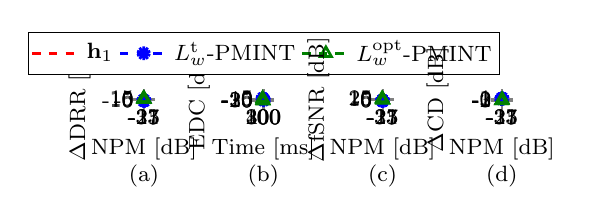
\begin{tikzpicture}[font = \footnotesize]

\begin{axis}[%
name = drr,
width=0.44\figurewidth,
height=0.9\figureheight,
scale only axis,
xmin=-35,
xmax=-13,
xlabel={NPM [dB]  \\ (a)},
xlabel absolute,
xlabel style={yshift=0.5em, align = center},
xtick = {-33,-27,-21,-15,-9,-3},
xticklabels = {-33,-27,-21,-15,-9,-3},
xmajorgrids,
ymin=-13,
ymax=18,
ytick = {-20,-15,-10,-5,0,5,10,15},
yticklabels = {-20,-15,-10,-5,0,5,10,15},
ylabel={$\Delta$DRR [dB]},
ylabel absolute, ylabel style={yshift=-1.2em},
ymajorgrids,
legend style={draw=black,fill=white,legend cell align=left}
]
\addplot [
color=blue,
dashed,
line width=1.0pt,
mark=10-pointed star,
mark size = 2.5pt,
mark options={solid}
]
table[row sep=crcr]{
-33 -7.02470757218629\\
-30 -8.14443505781971\\
-27 -7.1121604057721\\
-24 -10.4714130743616\\
-21 -10.2821001791262\\
-18 -9.15483519059332\\
-15 -10.6908486597571\\
};

\addplot [
color=green!50!black,
dashed,
line width=1.0pt,
mark=triangle,
mark size = 2.3pt,
mark options={solid}
]
table[row sep=crcr]{
-33 15.2577430337634\\
-30 13.7662744321774\\
-27 11.9108169599683\\
-24 10.523804780062\\
-21 10.0246030241427\\
-18 8.62811530047568\\
-15 7.80287789620582\\
};
\end{axis}

\begin{axis}[%
name = edc,
width=0.44\figurewidth,
height=0.9\figureheight,
scale only axis,
xmin=0,
xmax=400,
xlabel={Time [ms]  \\ (b)},
xlabel absolute,
xlabel style={yshift=0.5em, align = center},
xmajorgrids,
ymin=-30,
ymax=0,
ylabel={EDC [dB]},
ytick = {-30,-25,-20,-15,-10,-5,0},
yticklabels = {-30,-25,-20,-15,-10,-5,0},
ylabel absolute, ylabel style={yshift=-1.2em},
at={($(drr.south east)+(1.5cm,0cm)$)},
ymajorgrids,
legend style={at={([yshift=0.3cm] $(drr.north west)!1.2!(drr.north east)$)},anchor=south,row sep = -1pt,draw=black,fill=white,legend cell align=left, inner sep = 1pt},
    legend cell align=left,
    legend columns=5
]
\addplot [
color=red,
dashed,
line width = 1pt,
]
table[row sep=crcr]{
0 0\\
6.25080282594733 -1.71917450529903\\
12.5016056518947 -2.3578638928626\\
18.752408477842 -2.77197671476469\\
25.0032113037893 -3.13335302699001\\
31.2540141297367 -3.66734639526669\\
37.504816955684 -4.11764249612898\\
43.7556197816313 -4.48456676455284\\
50.0064226075787 -4.90005069914123\\
56.257225433526 -5.48266407790397\\
62.5080282594733 -6.0831136402403\\
68.7588310854207 -6.77176251137186\\
75.009633911368 -7.23701610867414\\
81.2604367373153 -7.71936993787205\\
87.5112395632627 -8.34445319218869\\
93.76204238921 -8.77918326681407\\
100.012845215157 -9.49813439295266\\
106.263648041105 -9.86669519386881\\
112.514450867052 -10.3389939823064\\
118.765253692999 -10.8875551760527\\
125.016056518947 -11.2014743370759\\
131.266859344894 -11.6128113981329\\
137.517662170841 -12.1312756047992\\
143.768464996789 -12.6782545265511\\
150.019267822736 -13.0773322458211\\
156.270070648683 -13.6207226643151\\
162.520873474631 -14.1289719904839\\
168.771676300578 -14.5674055115473\\
175.022479126525 -15.0433917911136\\
181.273281952473 -15.5098111695264\\
187.52408477842 -15.9636424296672\\
193.774887604367 -16.4246671255823\\
200.025690430315 -16.8425311599511\\
206.276493256262 -17.4452184159098\\
212.527296082209 -17.7810762798027\\
218.778098908157 -18.0784523200917\\
225.028901734104 -18.5384973538673\\
231.279704560051 -19.0684221088547\\
237.530507385999 -19.4567735521261\\
243.781310211946 -20.0376893545713\\
250.032113037893 -20.5150436881993\\
256.282915863841 -21.3835423093952\\
262.533718689788 -21.8617046720568\\
268.784521515735 -22.3118496672819\\
275.035324341683 -22.7483998414761\\
281.28612716763 -23.1097644336596\\
287.536929993577 -23.6567791052015\\
293.787732819525 -24.1427397729321\\
300.038535645472 -24.495231666475\\
306.289338471419 -25.0909537220336\\
312.540141297367 -25.5389390881714\\
318.790944123314 -26.0345343447452\\
325.041746949261 -26.5777278112269\\
331.292549775209 -27.1158434553079\\
337.543352601156 -27.5864257398906\\
343.794155427103 -27.9039117975341\\
350.044958253051 -28.3973998502722\\
356.295761078998 -28.9560010640739\\
362.546563904945 -29.4954699682026\\
368.797366730893 -29.9658175078164\\
375.04816955684 -30.3904843260426\\
};
\addlegendentry{$\mathbf{h}_1$};
\addplot [
color=blue,
dashed,
line width=1.0pt,
mark = 10-pointed star,
mark repeat=8,
mark size = 2.5pt,
mark options={solid}
]
table[row sep=crcr]{
0 0\\
6.25080282594733 -0.402392445535001\\
12.5016056518947 -0.586767738602906\\
18.752408477842 -0.674421744449907\\
25.0032113037893 -0.836601483041186\\
31.2540141297367 -0.982798579063373\\
37.504816955684 -1.22090944187144\\
43.7556197816313 -1.41388242642914\\
50.0064226075787 -1.6104429879991\\
56.257225433526 -1.90943044817842\\
62.5080282594733 -2.23351444123467\\
68.7588310854207 -2.57719229306877\\
75.009633911368 -2.76330519099706\\
81.2604367373153 -3.03983943429956\\
87.5112395632627 -3.39044109536333\\
93.76204238921 -3.73094942146284\\
100.012845215157 -3.97979123120212\\
106.263648041105 -4.28967974212387\\
112.514450867052 -4.73206964545856\\
118.765253692999 -5.15487420740395\\
125.016056518947 -5.60333883904464\\
131.266859344894 -6.04427457186193\\
137.517662170841 -6.31100410455234\\
143.768464996789 -6.64236986745887\\
150.019267822736 -7.11845911046745\\
156.270070648683 -7.39947374244033\\
162.520873474631 -7.60996632178938\\
168.771676300578 -7.87106774409726\\
175.022479126525 -8.259410718895\\
181.273281952473 -8.82371854732826\\
187.52408477842 -9.42286723756853\\
193.774887604367 -9.92725453611491\\
200.025690430315 -10.3832599432998\\
206.276493256262 -10.6900727821125\\
212.527296082209 -11.2687473921344\\
218.778098908157 -11.6652658781434\\
225.028901734104 -12.1305001512898\\
231.279704560051 -12.5236003982136\\
237.530507385999 -12.8640461219003\\
243.781310211946 -13.1735030392892\\
250.032113037893 -13.7711173507429\\
256.282915863841 -14.2013867864978\\
262.533718689788 -14.8935862609329\\
268.784521515735 -15.4651863073818\\
275.035324341683 -15.9668971191848\\
281.28612716763 -16.4946630440837\\
287.536929993577 -16.9804423090604\\
293.787732819525 -17.2754930151334\\
300.038535645472 -17.5428923485683\\
306.289338471419 -18.0632328601718\\
312.540141297367 -18.6207710173205\\
318.790944123314 -19.069453816918\\
325.041746949261 -19.6075969109912\\
331.292549775209 -20.3878978070272\\
337.543352601156 -20.6772502748103\\
343.794155427103 -21.268086925356\\
350.044958253051 -21.5872386217585\\
356.295761078998 -22.0163971736799\\
362.546563904945 -22.5634228382182\\
368.797366730893 -23.0865536076085\\
375.04816955684 -23.5757290835669\\
381.298972382787 -24.2568939826132\\
387.549775208735 -25.0922920328745\\
393.800578034682 -25.7910635641755\\
400.051380860629 -26.1106785189706\\
};
\addlegendentry{$L^{\rm t}_w$-PMINT};

\addplot [
color=green!50!black,
dashed,
mark=triangle,
mark size = 2.3pt,
mark options={solid},
mark repeat = 5,
line width=1.0pt,
]
table[row sep=crcr]{
0 0\\
6.25080282594733 -5.86848307225872\\
12.5016056518947 -12.4366852584372\\
18.752408477842 -18.7930997165107\\
25.0032113037893 -18.9054178862756\\
31.2540141297367 -19.0658094700046\\
37.504816955684 -19.3113060803179\\
43.7556197816313 -19.7897168445246\\
50.0064226075787 -20.1726429469802\\
56.257225433526 -20.6266348195759\\
62.5080282594733 -21.0393794404694\\
68.7588310854207 -21.181005101944\\
75.009633911368 -21.4891264264003\\
81.2604367373153 -21.7962013723806\\
87.5112395632627 -22.0971917266315\\
93.76204238921 -22.3453564290697\\
100.012845215157 -23.3036388495707\\
106.263648041105 -23.4481614974462\\
112.514450867052 -24.0635284407277\\
118.765253692999 -24.187041262648\\
125.016056518947 -24.4846097652299\\
131.266859344894 -24.7814974081539\\
137.517662170841 -25.0146480916989\\
143.768464996789 -25.5787253534042\\
150.019267822736 -25.9061434926005\\
156.270070648683 -26.2496038485734\\
162.520873474631 -26.4891532808286\\
168.771676300578 -26.8261023106667\\
175.022479126525 -27.3134595158724\\
181.273281952473 -28.2910743580883\\
187.52408477842 -28.9153078546925\\
193.774887604367 -29.4626581842887\\
200.025690430315 -29.9631729540118\\
206.276493256262 -30.1895942611621\\
};
\addlegendentry{$L^{\rm opt}_w$-PMINT};

\end{axis}

\begin{axis}[%
name = snr,
width=0.44\figurewidth,
height=0.9\figureheight,
scale only axis,
xmin=-35,
xmax=-13,
xlabel={NPM [dB]  \\ (c)},
xlabel absolute,
xlabel style={yshift=0.5em, align = center},
xtick = {-33,-27,-21,-15,-9,-3},
xticklabels = {-33,-27,-21,-15,-9,-3},
xmajorgrids,
ymin=-6,
ymax=20,
ytick = {-5,0,5,10,15,20},
yticklabels = {-5,0,5,10,15,20},
ylabel={$\Delta$fSNR [dB]},
ylabel absolute, ylabel style={yshift=-1.2em},
ymajorgrids,
at={($(edc.south east)+(1.5cm,0cm)$)},
]
\addplot [
color=blue,
dashed,
line width=1.0pt,
mark=10-pointed star,
mark size = 2.5pt,
mark options={solid}
]
table[row sep=crcr]{
-33 -3.88738222021021\\
-30 -3.93887661968727\\
-27 -4.13721313150292\\
-24 -4.13440406788482\\
-21 -5.12484879693002\\
-18 -3.53477709228735\\
-15 -4.36340190318735\\
};
\addplot [
color=green!50!black,
dashed,
line width=1.0pt,
mark=triangle,
mark size = 2.3pt,
mark options={solid}
]
table[row sep=crcr]{
-33 17.8228740222951\\
-30 11.433962470954\\
-27 7.73199959934204\\
-24 7.22531277668461\\
-21 7.81528247505952\\
-18 4.84143341321773\\
-15 3.66769650787159\\
};
\end{axis}

\begin{axis}[%
name = cd,
width=0.44\figurewidth,
height=0.9\figureheight,
scale only axis,
xmin=-35,
xmax=-13,
xlabel={NPM [dB]  \\ (d)},
xlabel absolute,
xlabel style={yshift=0.5em, align = center},
xtick = {-33,-27,-21,-15,-9,-3},
xticklabels = {-33,-27,-21,-15,-9,-3},
xmajorgrids,
ymin=-3,
ytick = {-3,-2,-1,0,1,2},
yticklabels  = {-3,-2,-1,0,1,2},
ymax=1.5,
ylabel={$\Delta$CD [dB]},
ylabel absolute, ylabel style={yshift=-1.2em},
at={($(snr.south east)+(1.5cm,0cm)$)},
ymajorgrids
]
\addplot [
color=blue,
dashed,
line width=1.0pt,
mark=10-pointed star,
mark size = 2.5pt,
mark options={solid}
]
table[row sep=crcr]{
-33 0.66843365612062\\
-30 0.423342074129967\\
-27 0.983498396934319\\
-24 1.14534372216349\\
-21 1.09619389186272\\
-18 1.10080369960071\\
-15 1.24771187572304\\
};
\addplot [
color=green!50!black,
dashed,
line width=1.0pt,
mark=triangle,
mark size = 2.3pt,
mark options={solid}
]
table[row sep=crcr]{
-33 -2.69429139279674\\
-30 -2.40144336503949\\
-27 -2.12513938804023\\
-24 -1.73938726762277\\
-21 -1.46334242727722\\
-18 -1.21369878690206\\
-15 -0.8545412126563\\
};
\end{axis}

\end{tikzpicture}%
\caption{Performance of the PMINT technique using the conventional filter length $L^{\rm t}_w$ and the intrusively determined optimal filter length $L^{\rm opt}_w$ for acoustic system $S_1$ in terms of (a) $\Delta$DRR, (b) EDC for an exemplary NPM of $-33$ dB, (c) $\Delta$fSNR, and (d) $\Delta$CD.}
\label{fig: pmint_lpmint}
\end{figure*}

\emph{MINT using $L^{\rm t}_w$ and $L_w^{\rm opt}$.} \enspace Figure~\ref{fig: mint_lmint} depicts the performance of the MINT technique when using the filter lengths $L^{\rm t}_w$ and $L_w^{\rm opt}$ in terms of $\Delta$DRR, EDC, $\Delta$fSNR, and $\Delta$CD.
As expected, the $\Delta$DRR values presented in Figure~\ref{fig: mint_lmint}(a) show that using the conventional filter length $L^{\rm t}_w$ in MINT fails to suppress the reverberant energy, even worsening the DRR by an average of $15$ dB in comparison to $\mathbf{h}_1$.
Furthermore, it can be observed that using the shorter filter length $L^{\rm opt}_w$ significantly increases the robustness of MINT for all NPMs, improving the DRR by an average of $4$ dB in comparison to $\mathbf{h}_1$.
These results are confirmed in Figure~\ref{fig: mint_lmint}(b), which depicts the EDC of $\mathbf{h}_1$ and the EDCs of the EIRs obtained using MINT with $L^{\rm t}_w$ and $L^{\rm opt}_w$ for an exemplary NPM of $-33$ dB.
It can be observed that while using $L^{\rm t}_w$ completely fails to achieve dereverberation and results in a slower reverberant energy decay rate than $\mathbf{h}_1$, using $L^{\rm opt}_w$ yields a significantly faster reverberant energy decay rate.
However, using $L^{\rm opt}_w$ yields only a slight improvement of the reverberant energy decay rate when compared to $\mathbf{h}_1$, even for the moderate NPM value of $-33$ dB.
Again as expected, the $\Delta$fSNR and $\Delta$CD values depicted in Figures~\ref{fig: mint_lmint}(c) and \ref{fig: mint_lmint}(d) show that using the conventional filter length $L^{\rm t}_w$ in MINT yields a significantly worse quality than the unprocessed microphone signal $x_1(n)$ for all NPMs.
While an increase in robustness is obtained for all NPMs using $L^{\rm opt}_w$, the performance in terms of the $\Delta$fSNR is still worse than for the unprocessed microphone signal $x_1(n)$.

Therefore as expected from the theoretical analysis in Section~\ref{sec: cond_no}, these simulation results validate that using a shorter reshaping filter than conventionally used in MINT is advantageous to increase the robustness against RIR perturbations. 
However, since acoustic system inversion using MINT is very sensitive to RIR perturbations, even a shorter reshaping filter is not sufficient to make the MINT technique fully robust against RIR perturbations.

\emph{RMCLS using $L^{\rm t}_w$ and $L_w^{\rm opt}$.} \enspace Figure~\ref{fig: rmcls_lrmcls} depicts the performance of the RMCLS technique using the filter lengths $L^{\rm t}_w$ and $L_w^{\rm opt}$ in terms of $\Delta$DRR, EDC, $\Delta$fSNR, and $\Delta$CD.
The $\Delta$DRR values presented in Figure~\ref{fig: rmcls_lrmcls}(a) show that for moderate NPMs using the conventional filter length $L^{\rm t}_w$ in RMCLS slightly suppresses the reverberant energy, whereas for NPMs larger than $-21$~dB using $L^{\rm t}_w$ in RMCLS fails to achieve dereverberation and worsens the DRR in comparison to $\mathbf{h}_1$.
Furthermore, it can be observed that using the optimal reshaping filter length $L^{\rm opt}_w$ significantly increases the reverberant energy suppression, yielding on average a $6$ dB larger $\Delta$DRR in comparison to the $\Delta$DRR obtained using $L^{\rm t}_w$.
To evaluate the reverberant energy decay rate, Figure~\ref{fig: rmcls_lrmcls}(b) depicts the EDC of $\mathbf{h}_1$ and the EDCs of the EIRs obtained using RMCLS with $L^{\rm t}_w$ and $L^{\rm opt}_w$ for an exemplary NPM of $-33$ dB.
It can be observed that for this moderate NPM, a very similar reverberant energy decay rate is obtained for the RMCLS technique when using $L^{\rm t}_w$ and $L^{\rm opt}_w$. 
Since the RMCLS technique using the conventional filter length $L^{\rm t}_w$ is rather robust yielding a fast reverberant energy decay rate, a shorter reshaping filter does not yield any improvement in the reverberant energy decay rate, but instead leads to a significant improvement in the perceptual speech quality.
This is illustrated in Figures~\ref{fig: rmcls_lrmcls}(c) and~\ref{fig: rmcls_lrmcls}(d), which shows that using $L^{\rm opt}_w$ in RMCLS significantly improves the $\Delta$fSNR and $\Delta$CD for all NPMs.

Therefore as expected from the theoretical analysis in Section~\ref{sec: cond_no}, these simulation results demonstrate that using a shorter reshaping filter than conventionally used in RMCLS is advantageous and increases the robustness against RIR perturbations.
\begin{table*}[t!]
\def\tabcolsep{3pt}
\begin{center}
  \caption{Average performance of the MINT, RMCLS, and PMINT techniques using the optimal reshaping filter length $L^{\rm opt}_w$.}
  \label{tbl: opt_Lw}
  \begin{tabularx}{\linewidth}{Xrrrrrrrrr}
    \toprule
    & \multicolumn{3}{c}{$S_1$} & \multicolumn{3}{c}{$S_2$} & \multicolumn{3}{c}{$S_3$} \\
    \midrule
      & $\Delta$DRR [dB] & $\Delta$fSNR [dB] & $\Delta$CD [dB] & $\Delta$DRR [dB] & $\Delta$fSNR [dB] & $\Delta$CD [dB] & $\Delta$DRR [dB] & $\Delta$fSNR [dB] & $\Delta$CD [dB] \\
    \midrule
       $L^{\rm opt}_{w}$-MINT & $3.69$ & $-0.55$ & $-1.31$ & $1.25$ & $-2.07$ & $0.07$ & $0.42$ & $-3.89$ & $-0.22$ \\
       $L^{\rm opt}_{w}$-RMCLS & $\bf{11.68}$ & $3.53$ & $-1.77$ & $3.57$ & $-0.81$ & $-0.39$ & $3.96$ & $-0.61$ & $-0.52$\\
       $L^{\rm opt}_{w}$-PMINT & $11.13$ & $\bf{8.65}$ & $\bf{-1.78}$ & $\bf{5.99}$ & $\bf{2.58}$ & $\bf{-0.66}$ & $\bf{4.33}$ & $\bf{1.88}$ & $\bf{-0.57}$ \\
    \bottomrule
  \end{tabularx}
\end{center}
\end{table*}
\begin{table*}[t!]
\def\tabcolsep{3pt}
\begin{center}
  \caption{Average performance of the PMINT technique using the automatically non-intrusively determined reshaping filter length $L^{\rm auto}_w$.}
  \label{tbl: auto_Lw}
  \begin{tabularx}{\linewidth}{Xrrrrrrrrr}
    \toprule
    & \multicolumn{3}{c}{$S_1$} & \multicolumn{3}{c}{$S_2$} & \multicolumn{3}{c}{$S_3$} \\
    \midrule
      & $\Delta$DRR [dB] & $\Delta$fSNR [dB] & $\Delta$CD [dB] & $\Delta$DRR [dB] & $\Delta$fSNR [dB] & $\Delta$CD [dB] & $\Delta$DRR [dB] & $\Delta$fSNR [dB] & $\Delta$CD [dB] \\
    \midrule
%       $L^{\rm auto}_{w}$MINT & $1.92$ & $-1.15$ & $-1.09$ & $-9.93$ & $-5.36$ & $1.17$ & $-5.55$ & $-6.64$ & $0.57$ \\
%       $L^{\rm auto}_{w}$RMCLS & $9.70$ & $1.41$ & $-1.33$ & $0.25$ & $-4.91$ & $0.51$ & $1.76$ & $-4.40$ & $0.04$\\
       $L^{\rm auto}_{w}$-PMINT & $10.58$ & $7.90$ & $-1.68$ & $4.41$ & $1.62$ & $-0.33$ & $3.34$ & $0.14$ & $-0.29$ \\
    \bottomrule
  \end{tabularx}
\end{center}
\end{table*}

\emph{PMINT using $L^{\rm t}_w$ and $L_w^{\rm opt}$.} \enspace Figure~\ref{fig: pmint_lpmint} depicts the performance of the PMINT technique using the filter lengths $L^{\rm t}_w$ and $L_w^{\rm opt}$ in terms of $\Delta$DRR, EDC, $\Delta$fSNR, and $\Delta$CD.
As expected, the $\Delta$DRR values presented in Figure~\ref{fig: pmint_lpmint}(a) show that the PMINT technique using the conventionally used filter length $L^{\rm t}_w$ fails to suppress the reverberant energy, even worsening the DRR in comparison to $\mathbf{h}_1$.
Furthermore, it can be observed that using $L^{\rm opt}_w$ in PMINT significantly increases the robustness for all NPMs, improving the DRR by an average of $11$ dB in comparison to $\mathbf{h}_1$.
These results are further confirmed in Figure~\ref{fig: pmint_lpmint}(b), which depicts the EDC of $\mathbf{h}_1$ and the EDCs of the EIRs obtained using PMINT with $L^{\rm t}_w$ and $L^{\rm opt}_w$ for an exemplary NPM of $-33$ dB.
It can be observed that the PMINT technique using $L^{\rm t}_w$ completely fails to achieve dereverberation and even results in a slower reverberant energy decay rate than $\mathbf{h}_1$.
Using the optimal reshaping filter length $L^{\rm opt}_w$ yields a significant increase in robustness, resulting in a much faster reverberant energy decay rate than $\mathbf{h}_1$.
Furthermore, the $\Delta$fSNR and $\Delta$CD values depicted in Figures~\ref{fig: pmint_lpmint}(c) and~\ref{fig: pmint_lpmint}(d) show that while PMINT using $L^{\rm t}_w$ worsens the perceptual speech quality in comparison to the unprocessed microphone signal $x_1(n)$, using $L^{\rm opt}_w$ results in a significantly better performance.

Therefore as expected from the theoretical analysis in Section~\ref{sec: cond_no}, decreasing the reshaping filter length in PMINT results in a significant increase in robustness against RIR perturbations, both in terms of reverberant energy suppression and perceptual speech quality improvement.


\subsection{Performance of equalization techniques when using the optimal intrusive reshaping filter length}
\label{sec: lcomp}
Since it was shown in the previous section that using a shorter reshaping filter than conventionally used increases the robustness of the considered equalization techniques in terms of all performance measures, in this section the performance of the MINT, RMCLS, and PMINT techniques using the optimal intrusively determined filter length $L^{\rm opt}_w$ is extensively compared for all acoustic systems in Table~\ref{tbl: ac_sys} and all NPMs in~(\ref{eq: npm}).
The performance of the different techniques is evaluated in terms of $\Delta$DRR, $\Delta$fSNR and $\Delta$CD, and the presented performance measures are averaged over all considered NPMs.

Table~\ref{tbl: opt_Lw} presents the obtained $\Delta$DRR, $\Delta$fSNR, and $\Delta$CD for all considered techniques\footnote{It should be noted that the performance measures presented for system $S_1$ are an average of the results already presented in Section~\ref{sec: robustness_increase}.}.
First it can be observed that the MINT technique using $L^{\rm opt}_w$ results in the lowest performance in terms of all performance measures, often worsening the perceptual speech quality in comparison to the unprocessed microphone signal $x_1(n)$.
Since the MINT technique is very sensitive to RIR perturbations~(cf. Figure~\ref{fig: mint_lmint}), the robustness increase that can be obtained by using a shorter reshaping filter length is also limited.
Second it can be observed that the RMCLS and PMINT techniques using $L^{\rm opt}_w$ result in a high reverberant energy suppression in terms of $\Delta$DRR, with the PMINT technique outperforming the RMCLS technique for system $S_2$ whereas a similar performance is obtained for systems $S_1$ and $S_3$.
Finally it can be observed that for all considered acoustic systems the PMINT technique using the reshaping filter length $L^{\rm opt}_w$ yields the highest perceptual speech quality improvement, outperforming the RMCLS technique in terms of $\Delta$fSNR.
While the PMINT technique always improves the perceptual speech quality in comparison to the unprocessed microphone signal $x_1(n)$, the RMCLS technique might fail to yield an improvement, as indicated by the negative $\Delta$fSNR for systems $S_2$ and $S_3$.
The advantage of using the PMINT technique lies in its control of the early reflections in the EIR, hence better preserving the perceptual speech quality of the output signal.

In summary, it can be said that the PMINT technique using the optimal intrusively determined reshaping filter length $L^{\rm opt}_w$ is a robust and perceptually advantageous equalization technique, yielding a high reverberant energy suppression and outperforming all other considered techniques in terms of perceptual speech quality improvement.



\subsection{Performance of the PMINT technique when using the automatic non-intrusive reshaping filter length}
\label{sec: filt_auto}
In this section we investigate the performance of the PMINT technique when using the automatic non-intrusive and practically applicable procedure for determining the reshaping filter length $L^{\rm auto}_w$ (discussed in Section~\ref{sec: lauto}) instead of the optimal intrusively determined reshaping filter length $L^{\rm opt}_w$.
Similarly as in Section~\ref{sec: lcomp}, we consider all acoustic systems in Table~\ref{tbl: ac_sys} and all NPMs in~(\ref{eq: npm}).
For all reshaping filter lengths in~(\ref{eq: lws}) the matrix $\mathbf{W}\hat{\mathbf{H}}$ is constructed and the PMINT reshaping filter is designed.
Furthermore, in order to generate the parametric L-curve the condition number $\chi_{\mathbf{W}\hat{\mathbf{H}}}$ and the least-squares error $\|\mathbf{W}(\hat{\mathbf{H}}\mathbf{w}-\mathbf{c}_{\rm d}) \|^2_2$ is computed. 
Using the triangle method~\cite{Castellanos_2002}, the automatic reshaping filter length $L^{\rm auto}_w$ corresponding to the point of maximum curvature of the L-curve is determined.
The performance of the PMINT technique using $L^{\rm auto}_w$ is evaluated in terms of $\Delta$DRR, $\Delta$fSNR, and $\Delta$CD, and the presented performance measures are averaged over all considered NPMs.

Table~\ref{tbl: auto_Lw} presents the $\Delta$DRR, $\Delta$fSNR, and $\Delta$CD obtained using PMINT with $L^{\rm auto}_w$ for all considered acoustic systems.
It can be observed that using the automatic non-intrusively determined reshaping filter length in PMINT yields a high dereverberation performance, both in terms of reverberant energy suppression and perceptual speech quality improvement.
When comparing the performance measures presented in Table~\ref{tbl: auto_Lw} to the ones presented in Table~\ref{tbl: opt_Lw}, it can be said that the performance of PMINT when using $L^{\rm auto}_w$ is generally similar to the performance obtained when using $L^{\rm opt}_w$.
More precisely, the average performance degradation over all considered acoustic systems when using the automatic non-intrusively determined reshaping filter length $L^{\rm auto}_w$ instead of the optimal intrusively determined reshaping filter length $L^{\rm opt}_w$ is only $1.04$ dB in terms of $\Delta$DRR, $2.29$ dB in terms of $\Delta$fSNR, and $0.24$ dB in terms of $\Delta$CD.

In summary, the presented results show that the automatic non-intrusively determined reshaping filter length in PMINT yields a high performance in the presence of RIR perturbations, making the PMINT technique using a shorter reshaping filter length a robust, perceptually advantageous, and practically applicable technique.

\section{Conclusion}
In this paper we have proposed to use a shorter reshaping filter length than conventionally used in acoustic multi-channel equalization techniques, such that a better conditioned optimization criterion is obtained.
We have analytically shown that using a shorter reshaping filter decreases the condition number of the convolution matrix, increasing as a result the robustness against RIR perturbations.
In addition, we have proposed to automatically determine the reshaping filter length as the point of maximum curvature of the parametric plot of the condition number versus the least-squares error, such that both quantities are kept small.
Using instrumental measures, it has been shown that using shorter reshaping filters indeed increases the robustness of MINT, RMCLS, and PMINT against RIR perturbations.
In addition, it has been shown that PMINT using the optimal intrusively determined reshaping filter length outperforms MINT and RMCLS.
Finally, it has been shown that the automatic non-intrusive procedure for selecting the reshaping filter length in PMINT yields a nearly optimal performance, confirming the practical applicability of using shorter reshaping filters in acoustic multi-channel equalization.
\section*{Appendix A}
\label{app: sing_vals}
In order to construct the matrix $\mathbf{W}_s\hat{\mathbf{H}}_s$, we first create an intermediate $[p_{\rm t}-(L^{\rm t}_w-L^{\rm s}_w)] \times [q_{\rm t}-(L^{\rm t}_w-L^{\rm s}_w)]$-dimensional sub-matrix $\mathbf{T}$ by deleting $L^{\rm t}_w-L^{\rm s}_w$ rows and $L^{\rm t}_w-L^{\rm s}_w$ columns from $\mathbf{W}_{\rm t}\hat{\mathbf{H}}_{\rm t}$.
The interlacing inequalities in~(\ref{eq: inter_sing}) for the matrices $\mathbf{W}_{\rm t}\hat{\mathbf{H}}_{\rm t}$ and $\mathbf{T}$ can be written as
\begin{equation}
\label{eq: inter_singT}
\sigma_{\mathbf{W}_{\rm t}\hat{\mathbf{H}}_{\rm t}}(i) \geq \sigma_{\mathbf{T}}(i) \geq \sigma_{\mathbf{W}_{\rm t}\hat{\mathbf{H}}_{\rm t}}(i+(L^{\rm t}_w-L^{\rm s}_w)),
\end{equation}
for $i = 1, \; \ldots, \; r_{\rm t}-(L^{\rm t}_w-L^{\rm s}_w), \; \ldots, \; p_{\rm t}-(L^{\rm t}_w-L^{\rm s}_w)$.
Based on~(\ref{eq: inter_singT}), the following inequalities between the singular values of the matrices $\mathbf{W}_{\rm t}\hat{\mathbf{H}}_{\rm t}$ and $\mathbf{T}$ can be established:
\begin{align}
\label{eq: ineq1}
\sigma_{\mathbf{W}_{\rm t}\hat{\mathbf{H}}_{\rm t}}(1) & \geq \sigma_{\mathbf{T}}(1), \\
\label{eq: ineq2}
\sigma_{\mathbf{T}}(r_{\rm t}-(L^{\rm t}_w-L^{\rm s}_w)) &\geq \sigma_{\mathbf{W}_{\rm t}\hat{\mathbf{H}}_{\rm t}}(r_{\rm t}).
\end{align}
In order to construct the matrix $\mathbf{W}_{\rm s}\hat{\mathbf{H}}_{\rm s}$, $(M-1)(L^{\rm t}_w-L^{\rm s}_w)$ columns are now deleted from the matrix $\mathbf{T}$.
The interlacing inequalities in~(\ref{eq: inter_sing}) for the matrices $\mathbf{T}$ and $\mathbf{W}_{\rm s}\hat{\mathbf{H}}_{\rm s}$ can be written as
\begin{equation}
\label{eq: inter_singS}
\sigma_{\mathbf{T}}(i) \geq \sigma_{\mathbf{W}_{\rm s}\hat{\mathbf{H}}_{\rm s}}(i) \geq \sigma_{\mathbf{T}}(i+(M-1)(L^{\rm t}_w-L^{\rm s}_w)),  
\end{equation}
for $i = 1, \; \ldots, \; r_{\rm s}$.
Using~(\ref{eq: inter_singS}), the following inequalities between the singular values of the matrices $\mathbf{T}$ and $\mathbf{W}_{\rm s}\hat{\mathbf{H}}_{\rm s}$ can be written:
\begin{align}
\label{eq: ineq3}
\sigma_{\mathbf{T}}(1) & \geq \sigma_{\mathbf{W}_{\rm s}\hat{\mathbf{H}}_{\rm s}}(1), \\
\label{eq: ineq4}
\sigma_{\mathbf{W}_{\rm s}\hat{\mathbf{H}}_{\rm s}}(r_{\rm s}) & \geq \sigma_{\mathbf{T}}(r_{\rm s}+(M-1)(L^{\rm t}_w-L^{\rm s}_w)).
\end{align}
The index of the singular value in the right hand side of~(\ref{eq: ineq4}) can be written as
\begin{align}
\!\!\!\!\!\!\!\!\!& r_{\rm s}+(M-1)(L^{\rm t}_w-L^{\rm s}_w)  = ML^{\rm s}_w+(M-1)(L^{\rm t}_w-L^{\rm s}_w) \nonumber  \\
\label{eq: ineq5}
\!\!\!\!\!\!\!\!\!& = ML^{\rm t}_w - (L^{\rm t}_w - L^{\rm s}_w) \geq r_{\rm t} - (L^{\rm t}_w - L^{\rm s}_w),
\end{align}
with~(\ref{eq: ineq5}) clearly holding since the number of columns in $\mathbf{W}_{\rm t}\hat{\mathbf{H}}_{\rm t}$ is greater or equal than its rank, i.e.,
\begin{equation}
q_{\rm t} = ML^{\rm t}_w \geq p_{\rm t} \geq r_{\rm t}.
\end{equation}
Based on~(\ref{eq: ineq5}) and the fact that the singular values of the matrices are sorted in descending order, one can write
\begin{equation}
\label{eq: ineq6}
\sigma_{\mathbf{T}}(r_{\rm s}+(M-1)(L^{\rm t}_w-L^{\rm s}_w)) \geq  \sigma_{\mathbf{T}}(r_{\rm t} - (L^{\rm t}_w-L^{\rm s}_w)).
\end{equation}
Using~(\ref{eq: ineq6}), the inequality in~(\ref{eq: ineq4}) can also be written as
\begin{equation}
\label{eq: ineq77}
\sigma_{\mathbf{W}_s\hat{\mathbf{H}}_s}(r_s)  \geq \sigma_{\mathbf{T}}(r_{\rm t}-(L^{\rm t}_w-L^{\rm s}_w)).
\end{equation}
Finally, combining~(\ref{eq: ineq1}),~(\ref{eq: ineq2}),~(\ref{eq: ineq3}), and~(\ref{eq: ineq77}) the following inequalities relating the largest and smallest non-zero singular values of $\mathbf{W}_{\rm t}\hat{\mathbf{H}}_{\rm t}$ and $\mathbf{W}_s\hat{\mathbf{H}}_s$ can be established:
\begin{align}
\sigma_{\mathbf{W}_{\rm t}\hat{\mathbf{H}}_{\rm t}}(1) & \geq \sigma_{\mathbf{W}_{\rm s}\hat{\mathbf{H}}_{\rm s}}(1), \\
\sigma_{\mathbf{W}_{\rm s}\hat{\mathbf{H}}_{\rm s}}(r_{\rm s}) & \geq \sigma_{\mathbf{W}_{\rm t}\hat{\mathbf{H}}_{\rm t}}(r_{\rm t}).
\end{align}

\begin{backmatter}

\section*{Competing interests}
  The authors declare that they have no competing interests.

  \section*{Acknowledgments}
  This work was supported in part by the Cluster of Excellence 1077 ``Hearing4All'', funded by the German Research Foundation (DFG), the Marie Curie Initial Training Network DREAMS (Grant no. 316969), and the joint Lower Saxony-Israeli Project ATHENA, funded by the State of Lower Saxony.
  
\bibliographystyle{bmc-mathphys} 
\bibliography{ref}

%%%%%%%%%%%%%%%%%%%%%%%%%%%%%%%%%%%

\end{backmatter}
\end{document}
